\documentclass[12pt]{ociamthesis}  % default square logo 
%\documentclass[12pt,beltcrest]{ociamthesis} % use old belt crest logo
%\documentclass[12pt,shieldcrest]{ociamthesis} % use older shield crest logo

%load any additional packages
\usepackage{amssymb}
\usepackage{color}
\usepackage{amsmath,mathtools}
\usepackage[square,sort,comma,numbers]{natbib}
\graphicspath{{images/}}
\usepackage{graphicx,float,subcaption}
\usepackage[font=footnotesize]{caption}
\usepackage{makecell}
\usepackage{booktabs}
\usepackage{multirow}
\usepackage{hyperref}



%input macros (i.e. write your own macros file called mymacros.tex 
%and uncomment the next line)
%\include{mymacros}

\title{Analysis and optimization of \\[1ex]rib-stiffened vaulted floor for dynamic performance}   %note \\[1ex] is a line break in the title

\author{Hao Wu\\15-946-296}             %your name
% \college{Block Research Group}  %your college
\supervisor{Prof. Dr. Philippe Block\\Dr. Andrew Liew\\(ETH Zurich)}


%\renewcommand{\submittedtext}{change the default text here if needed}
\degree{Master of Science ETH in Bauingenieurwissenschaften}     %the degree
\degreedate{January 2019}         %the degree date

%end the preamble and start the document
\begin{document}

%this baselineskip gives sufficient line spacing for an examiner to easily
%markup the thesis with comments
\baselineskip=18pt plus1pt

%set the number of sectioning levels that get number and appear in the contents
\setcounter{secnumdepth}{3}
\setcounter{tocdepth}{3}


\maketitle                  % create a title page from the preamble info
% \begin{dedication}
This thesis is dedicated to\\
 someone\\
for some special reason\\
\end{dedication}        % include a dedication.tex file
% \include{acknowlegements}   % include an acknowledgements.tex file
\begin{abstract}
The rib-stiffened vaulted floor designed by the BLOCK Research Group at ETH Zurich can achieve adequate stiffness and bearing capacity with ultra-lightweight construction. For this statically well optimized floor, the dynamic behavior was still unknown. Natural frequency based traditional methods fail to assess its dynamic performance. The aim of this study is to obtain a fundamental understanding of the floor's dynamic behavior and to develop proper measures to improve its dynamic performance if it turns out to be unsatisfactory.

The analysis procedure for performance evaluation consists of the following steps: firstly, the generation of floor mesh models with different combinations of geometric parameters; secondly, the solution of dynamic response time history via modal superposition; finally, post-processing of the response based on the chosen guideline and comparison with acceptance criterion. After the performance evaluations of these floor models, qualitative and quantitative relations among the geometric parameters, modal parameters and dynamic performance were found and understood. 

It was shown that the most studied floor failed to meet the acceptance criterion. Two different approaches were taken to improve the performance of the floor. One was based on the acquired understanding of the mechanism behind the dynamic behavior from previous findings, the other adopted a machine learning alike idea and used a surrogate model for automatic optimization. Both approaches ended up with similar optimized figures and accomplished considerable improvements in dynamic performance. 

This thesis has revealed the dynamic characteristics of the rib-stiffened vaulted floor and possible ways to improve its dynamic performance. It may also have provided some insight into the dynamic behavior of general high frequency floors. 

 
\end{abstract}          % include the abstract
%\chapter*{Foreword}

\section{Acknowledgments}

\section{Personal motivation}


\begin{romanpages}          % start roman page numbering
\tableofcontents            % generate and include a table of contents
\listoffigures              % generate and include a list of figures
\listoftables
\end{romanpages}            % end roman page numbering

%now include the files of latex for each of the chapters etc
\chapter{Introduction}
\label{chap1}

\section{Vibration problems in modern buildings}
Modern buildings have been showing increasing demand for faster construction, larger bay size and more flexible work space use in recent years. This demand usually leads to long spans, lightweight floor systems and reduced dividing partitions. The associated reduction of flexural stiffness, self weight attributed to unit floor area and structural damping of the floors has aroused a greater awareness of potential vibration problems when subjected to human activities.

A Building with vibration problems may cause an apprehension for the structural safety, loss of mental concentration and an unwell feeling among the people working inside \cite{bachmann2012vibration}. Such buildings are prone to be subject to more complaints than others. Unfortunately, once the construction is finished, it is very difficult to improve its dynamic performance by structural measures later on, as such modification is only possible by making major changes to the mass, stiffness or damping of the floor system. Therefore, it is significant to consider the human-induced vibration of floors at the conceptual stage.

\section{Rib-stiffened vaulted floor}
The rib-stiffened vaulted floor designed by BLOCK Research Group at ETH Zurich conforms to the trend of lightweight floor systems in modern buildings, it may be also confronted with accompanying vibration problems. A prototype of the vaulted floor element designed for the NEST HiLo project is shown in figure \ref{fig:prototype}. This unreinforced concrete floor consists of a thin funicular vault stiffened by a series of spandrel walls on its extrados. The structural prototype is completed with tension ties, which link the supports and absorb the horizontal thrusts of the funicular shell.
\begin{figure}[H]
\begin{subfigure}[b]{.9\textwidth}
  \centering
  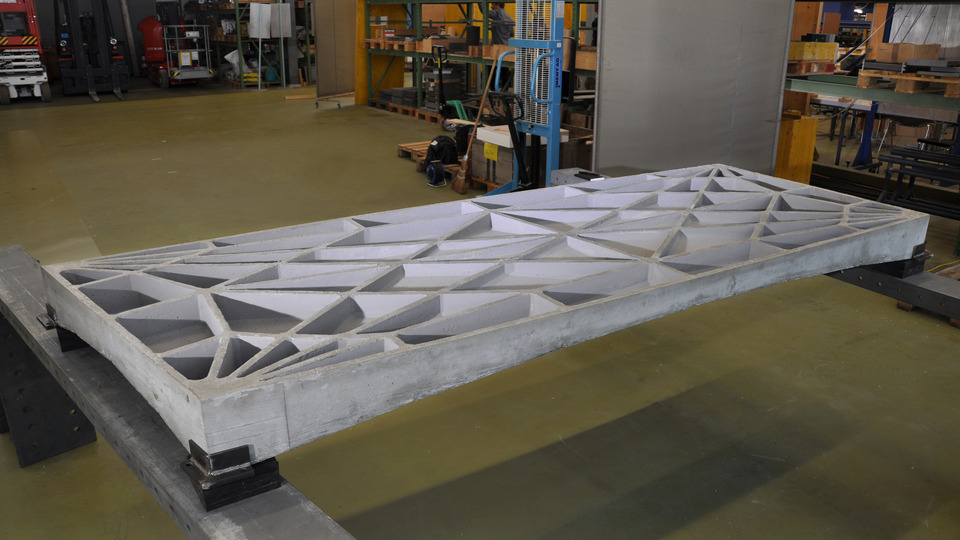
\includegraphics[width=.99\linewidth]{prototype1}
  \caption{The prototype before static experiment}
\end{subfigure}

\begin{subfigure}[b]{.9\textwidth}
  \centering
  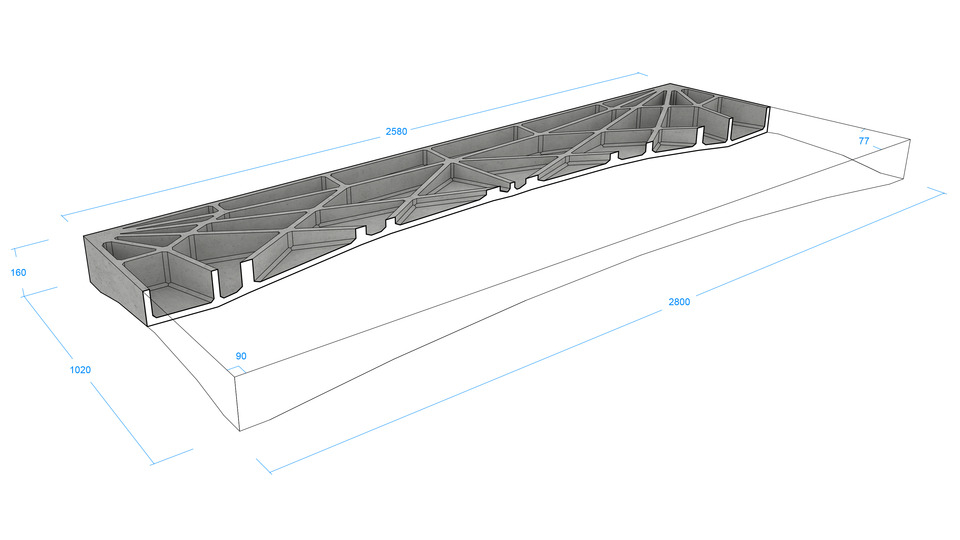
\includegraphics[width=.99\linewidth]{prototype2}
  \caption{Cross-section and dimensions}
\end{subfigure}

\caption{A prototype of the rib-stiffened valued floor \cite{prototype}}
\label{fig:prototype}
\end{figure}

The vaulted floor owns some unique geometric and modal features that differentiate itself from regular concrete and steel/concrete composite floors.
\begin{itemize}
    \item \textbf{Adequate stiffness achieved by ultra-lightweight construction}\\
    The geometry of the vault was found through the interactive form-finding process TNA (Thrust Network Analysis). Thanks to the inherent nature of TNA, the vault behaves as a compression-only shell under self-weight and dead load. The load transfer through compression is much more efficient than through bending. As a result, the floor would save more than 70\% of the weight compared to traditional, 25-30cm-thick concrete floor floors used in the construction of framed buildings and meanwhile keep deformations not higher than 1/500 of the span in the serviceability limit state \cite{lopez2014prototype}. 
    
    \item \textbf{High natural frequency}\\
    The high natural frequency is a direct consequence of the former feature. The natural frequency of a single degree of freedom system reads
    \begin{equation}
        f_n=\frac{1}{2\pi}\sqrt{\frac{k}{m}}
    \end{equation}
    It indicates that if the structure is so optimized that adequate stiffness remains while much mass is removed, the structure will show a high natural frequency. 
    
     The series of vaulted floors studied in this research (differ from this prototype in many aspects, but they share the same essential principles) have the fundamental natural frequencies ranging from 20 Hz to 100 Hz. The vaulted floor is a typical high frequency floor, in which resonant build up does not happen and the response is a series of rapidly decaying responses following each footfall. The cut-off frequency differentiating low frequency and high frequency floor is accepted by around 10 Hz \cite{smith2007design}\cite{willford2007predicting}. Then the vaulted floor would have been considered as very "dynamically stiff" when only judged from the aspect of the natural frequency.
    
    \item \textbf{Low modal mass}\\
    In the form-finding and optimization process of the vaulted floor much of its mass was removed from the middle, as it does not make much contribution to either stiffness or strength. On the contrary, a considerable amount of mass is distributed on the side due to the existence of stiffening ribs with high depth. Such muss distribution results in a very low modal mass. A solid rectangular floor has a modal mass of 25\% of the total mass (given that the mode shape is so normalized that the maximal item is 1) \cite{howard2007modal}, whereas only 1\%-7\% for a vaulted floor with constant thickness in both vault and ribs (see figure \ref{fig:geom-m12m}). 
    
    \item \textbf{Vault/ribs interaction}\\
    The ribs are intended to disperse the external load to vault and stiffen the vault locally in static cases. From the aspect of dynamics, the situation can be just the opposite. The vault has a more or less uniform mass distribution over the whole area, whereas the ribs have much higher mass and stiffness concentration near the edges. Therefore, the ribs are prone to vibrate locally in the middle with high amplitudes, the vault tends to stiffen the ribs in the middle and disperse the vibration to a larger region.
    
\end{itemize}

\section{Statement of problems}
Since the vaulted floor owns those unique features and their influences on its dynamic performance are not fully understood, or even not studied, there is an acute need for:
\begin{itemize}
    \item a fundamental understanding of the dynamic behavior of the vaulted floor
    \item improvement/optimization if the dynamic performance turns out to be unsatisfactory
\end{itemize}

\section{Objectives}
This study is limited to explore the dynamic performance of the vaulted floor under one person walking excitation. In pursuit of a fundamental understanding of its dynamic behavior, the following objectives must be firstly addressed in the study:
\begin{itemize}
    \item to develop an analysis procedure for dynamic response, allowing fast, accurate and robust solution of dynamic process;
    \item to implement suitable approaches for evaluation of vibration perception;
    \item to identify key parameters that influence the dynamic performance by parametric study and sensitivity analysis, more importantly, to understand how they influence and why they influence the performance in that way; and,
    \item to find qualitative and quantitative relations among geometry, modal property and dynamic performance. 
\end{itemize}

Based on the understanding obtained above, improvement/optimization can be achieved if the following objectives are realized:
\begin{itemize}
    \item to find the "best" mass and stiffness distribution under certain constraints (e.g. constant mass, allowable thickness ratio, etc.) either through oriented trial and error or automatic optimization; and,
    \item to consider and demonstrate the feasibility of attaining such mass and stiffness distribution in reality.
\end{itemize}


\section{Thesis structure}
This master's thesis is composed of 6 chapters.

Chapter 1 introduces the importance of the study on dynamic performance of floors in modern buildings and provides background information about the rib-stiffened vaulted floor. The statement of problems and objectives are defined.

Chapter 2 reviews the evaluation methods for the dynamic performance of floors and the state of the art in design codes and research.

Chapter 3 elaborates the methodology for the evaluation of dynamic performance. Basic modeling assumptions are clarified and analysis procedure for the dynamic response is introduced.

Chapter 4 delivers the results of dynamic analysis. The calibration of the results from modal superposition and from Abaqus is conducted. The rest of this chapter reveals the relations among geometric parameters, modal properties and dynamic performance. 

Chapter 5 presents two possible ways to improve the dynamic performance. One is based on the acquired understanding of the floor's dynamic behavior from previous analysis, the other is a surrogate model based automated optimization.

Chapter 6 concludes the main findings in this thesis with an outlook on further research possibilities. 




























\chapter{Literature review}
\label{chap2}

\section{Natural frequency based traditional evaluation methods}
Many factors play a role in the nature of floor vibrations in office and residential buildings under pedestrian excitation, among them the footfall loads, the configuration of partitions, furnishings, geometric shapes of floor area, etc. These factors not only influence the dynamic excitation, but also the modal characteristics of the floor. Rational calculations of vibration amplitudes induced by dynamic forces become rather complicated and uncertain. Consequently, empirical and semi-empirical natural frequency based methods have been developed to deal with this situation since decades \cite{bachmann2012vibration}.

For low-frequency floors whose first natural frequency is under 10 Hz, since the annoying vibration amplitudes are mainly caused by a coincidence of the natural frequency with the frequency of footfall forces, the problem can be solved by keeping these frequencies away from each other. That is the principal idea of "high tuning method", one of the most important and widely adopted empirical methods in last decades \cite{bachmann2012vibration}. Historically, designers have used the natural frequency of the floor as the sole measure of acceptable performance \cite{european1992eurocode}. In the United Kingdom, the traditional approach used to design conventional floors for serviceability criteria has been to check the primary and secondary beams independently for a minimum natural frequency of 4.0 Hz \cite{smith2007design}. A sufficiently high natural frequency means that a floor is effectively 'tuned' out of the frequency range of the primary harmonic components of the walking activity, thus it is warded off the likeliness of resonant behavior. 

\section{Performance based approaches}
Early acceptability criteria that were solely based on natural frequency cannot represent a realistic assessment of the vibration likely to arise in normal service. It therefore follows that ensuring a design meet certain minimum frequency limits may still result in a floor that is unacceptable in service. Conversely, some floors under such design frame could be over-conservative \cite{smith2007design}. The need for a more robust and comprehensive performance based approach became clear.

Within Europe, the following guidelines published by different research institutes provide the possibility to evaluate the dynamic performance of floors according to the response level: P354 by SCI (The Steel Construction Institute) \cite{smith2007design}, EUR 21972 by TSR (Technical Steel Research of European Commission) \cite{sedlacek2006generalisation}, EUR 24084 by JRC (Joint Research Center of European Commission) \cite{feldmann2009design} and HiVoSS guideline by RFCS (Research Fund for Coal and Steel) \cite{feldmann2010human}. 

These guidelines help assess the dynamic performance by providing stipulation of the dynamic excitation input, clarification of response assessment process, suggestion for the acceptability criteria and examples of practical application. Based on these guidelines, it is possible to conduct a simplified evaluation with hand calculation for a regular floor as well as a complex assessment with FE modeling and response time history analysis for an unconventional floor.

They have achieved agreement in the primary process of performance assessment. They all respect the fact that human body's sensitivity to a given amplitude of vibration changes with the frequency of vibration, the frequency weighting function for response evaluation is therefore introduced. Moreover, it is differentiated between low frequency and high frequency floors. They nonetheless deal with the uncertainty in dynamic excitation differently, JRC and Hivoss adopt a probabilistic manner to describe the uncertainty in footfall amplitude and frequency, while SCI and TSR simplify the dynamic excitation as a series of deterministic values varying with time. Another difference lies in the choice of representative value of response. TSR uses both acceleration and velocity, whereas SCI only acceleration, JRC and Hivoss only velocity. Due to these distinctions the classification of vibration perception varies from one to another as well.

The evaluation guideline P354 by SCI is selected to be performed for the dynamic performance assessment in this study for three main reasons. Firstly, the stochastic process adopted by JRC and Hivoss is unnecessarily complicated and computationally intensive. In addition, the deterministic relation between input and output can help unveil the hidden associations. Secondly, the assumption of footfall input in TSR is believed to be too conservative (40\% higher than that of SCI), especially when combined with a series of conservative modeling assumptions. Finally, the SCI document provide users with important and useful hints for modeling and implementation, it also seems to have gained more practical applications an citations than other guidelines.


\section{State of the art in design codes and research}
Current European design codes do not give any certain natural frequency level above which the structure should be kept to avoid vibration problems, neither do they suggest any analysis approach for evaluation of the dynamic performance. The vibration of concrete structures, as a serviceability sate limit, is even not covered in Eurocode 2 (design of concrete structures) \cite{european2004eurocode2}. This may imply that for common concrete structures, vibration is not a noticeable problem. In Eurocode 3 (design of steel structures)  and Eurocode 4 (design of composite steel and concrete structures) , requirements for vibrations should be specified for each project and agreed with the client \cite{european2005eurocode3}\cite{european2004eurocode4}.

Varieties of research have investigated dynamic performances of different regular floor systems. But only few of them have addressed high frequency floors and give referential hints about how geometry and modal properties influence the dynamic performance.  

Arup has conducted a series of research and compared the relative vibration performance of different forms of construction (reinforced concrete, pre-stressed concrete and concrete/steel composite) for hospital use \cite{arup2004hospital}. it is concluded that Of the floors that have been designed to meet strength and deflection criteria only, the dynamic performance of the concrete designs is significantly better than that of the composite designs. It further points out that although the natural frequency is an important dynamic parameter, it does not necessarily follow that a floor with a higher frequency will have a lower dynamic response. In fact the reverse may be true if the frequency is increased by removing mass . This finding indicates the possibility that when a floor is optimized towards a statically stiff and strong structure with little material (usually accompanied with a high natural frequency), it may still show vibration problems. Some other dynamic parameters other than natural frequency must play a role in the meanwhile. 

SCI P354 makes a clear distinction between low frequency floors and high frequency floors. Equation (51) in SCI P354, repeated in equation \ref{eqn:SCI} gives a useful clue of how natural frequency and modal mass influence the response acceleration in the transient phase for a simplified assessment for steel floors:
\begin{equation}
    a_{w,rms} = 2\pi\mu_e\mu_r\frac{185}{Mf_0^{0.3}}\frac{Q}{700}\frac{1}{\sqrt{2}}W
\label{eqn:SCI}
\end{equation}
\noindent
where $f_0$ is the fundamental frequency of the floor, $M$ is the modal mass. The inverse proportionality between response acceleration and $Mf_0^{0.3}$ means that the dynamic response can be reduced by raising modal mass and fundamental frequency with less effect from the latter term. It is nevertheless not clear, whether this expression holds only for the given structural form and for a simplified assessment. Unfortunately, there are also no further hints about how to alter the two correlated parameters in an expected direction.

Even less research has been performed for vaulted floors of any kind. A theoretical, experimental or empirical benchmark in terms of modal characteristics or dynamic response associated with vaulted floors is hard to find. Therefore, there exists a need, not only within the BLOCK Research Group for the NEST HiLo project soon to be built, but also for general high frequency floors whose high frequency is achieved by removing statically redundant material, to study their dynamic performance and crucial parameters that plays a role in it. The purpose of this study is restricted to evaluate and improve the dynamic performance of the rib-stiffened vaulted floor, but it may also provide a useful insight into the dynamic behavior of other types of high frequency floors.

\chapter{Methodology for evaluation of dynamic performance}
\label{chap3}

\section{General work flow}
Figure \ref{fig:workflow} illustrates the general work flow for the evaluation of dynamic performance. The first step is to create mesh models in Rhino with different combinations of geometric parameters. Then, the mesh models are exported in Abaqus for modal analysis. As a next step, modal parameters (natural frequencies, modal masses, modes shapes) from modal analysis are extracted to solve the response time history of the floor under footfall excitation via modal superposition. Once the response from each mode is available, post-processing of the response will be conducted based on the procedure presented by the evaluation guideline. Finally, the post-processed response will be compared with the acceptance criteria and a conclusion about the vibration level can be drawn.

\begin{figure}[H]
\centering
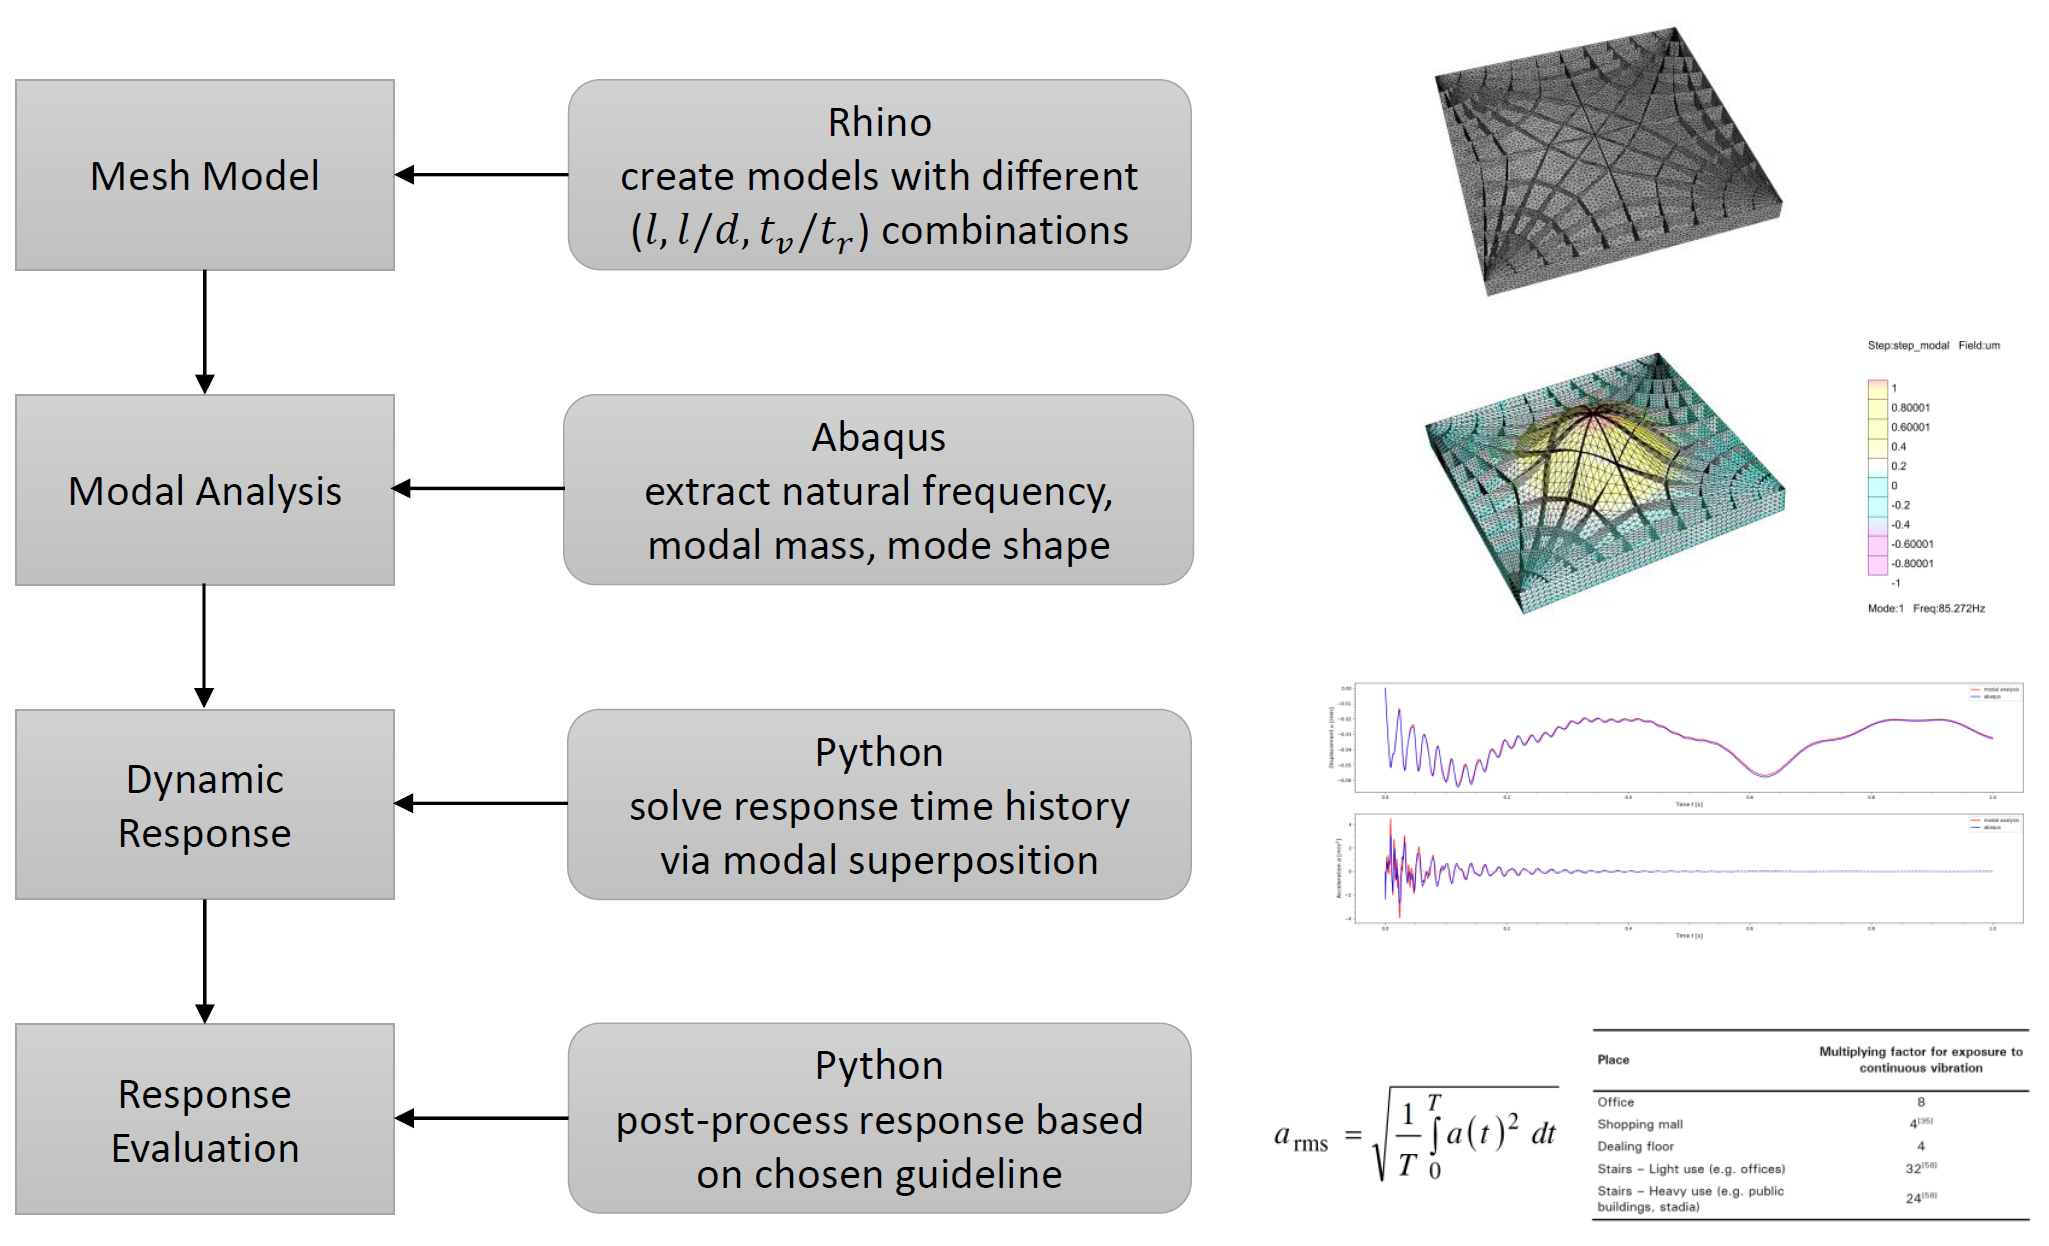
\includegraphics[width=1.0\textwidth]{workflow}
\caption{Work flow for evaluation of vibration}
\label{fig:workflow}
\end{figure}

\section{Modeling}
\subsection{Mesh model generation}
Three geometrical parameters are considered important to outline the geometry of a floor if the pattern of ribs is given: the span $l$, span/depth ratio $l/d$ and vault/ribs thickness ratio $t_v/t_r$. Some assumptions are made to avoid unnecessary complexity: the floor has a square form in plane; the vault has a constant thickness everywhere, so do the ribs, although vault and ribs can show different thicknesses; the top of the neutral surface of the vault is 5cm under the upper bound of the floor, this value does not change with the span. The three parameters have the following values covering realistic ranges in practical use as well as reasonably exaggerated ranges for research reasons:
\begin{align*}
    l&=[5,6,7,8,9,10]\quad[m]\\
    l/d&=[10,12.5,15,17.5,20]\quad[-]\\
    t_v/t_r&=[0.1,0.5,1,2,5,10]\quad[-]
\end{align*}

The geometry of the vault and ribs is form-found based on TNA and created with COMPAS\_TNA package. The span and depth of the floor is easy to scale, but the pattern of ribs not. To ensure that floors with different spans have similar ribs density (similar panel size surrounded by ribs), the numbers of ribs in both circular and radial directions are scaled in proportion to the span. The thickness of vault and ribs is given in form of thickness ratio under the condition that the floor mass equals to a constant value, no matter how the ratio varies. The floor mass is set to be 40\% of the mass of a solid rectangular one with the same outer geometry. If the total volume of the floor $v$, the area of the vault $a_v$ and ribs $a_r$, and thickness ratio $\gamma = t_v/t_r$ are known, the thickness of ribs and vault can be determined by
\begin{align}
    t_r &= \frac{v}{\gamma a_v+a_r}\\
    t_v &= \gamma t_r
\end{align}

Figure \ref{fig:mehs_models} shows the mesh models of floors with constant $l/d=15$ and all above listed spans. The combination of the three parameters will generate 180 models for analysis.

\begin{figure}[H]
\begin{subfigure}[b]{.48\textwidth}
  \centering
  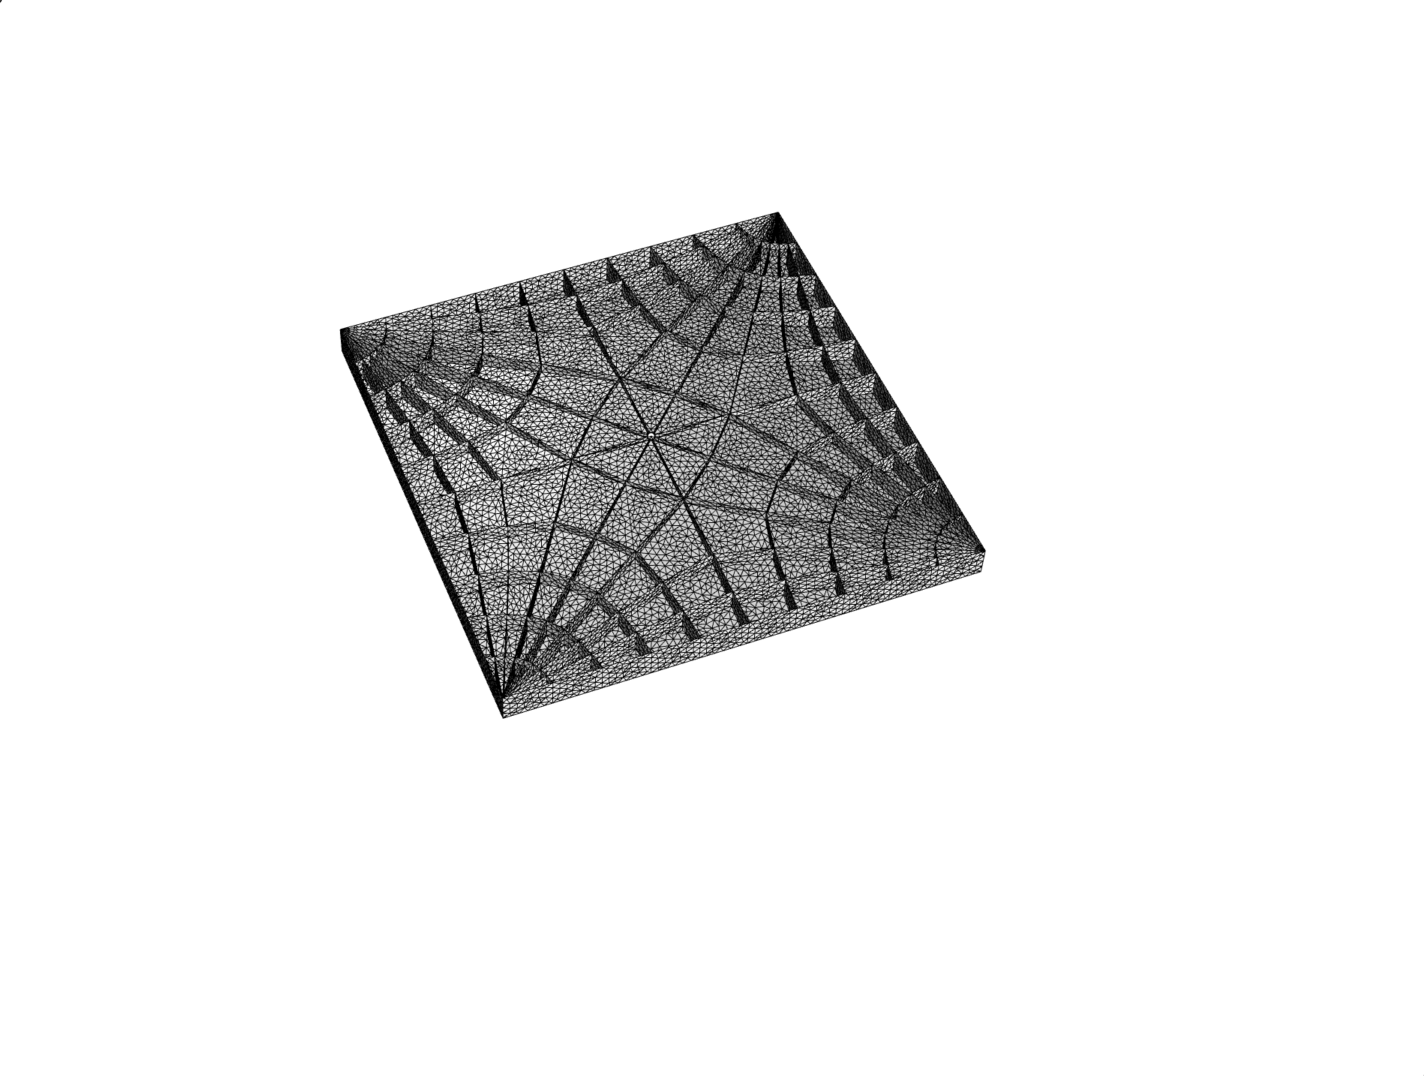
\includegraphics[width=.95\linewidth]{span5}
  \caption{span=5m}
\end{subfigure}
~
\begin{subfigure}[b]{.48\textwidth}
  \centering
  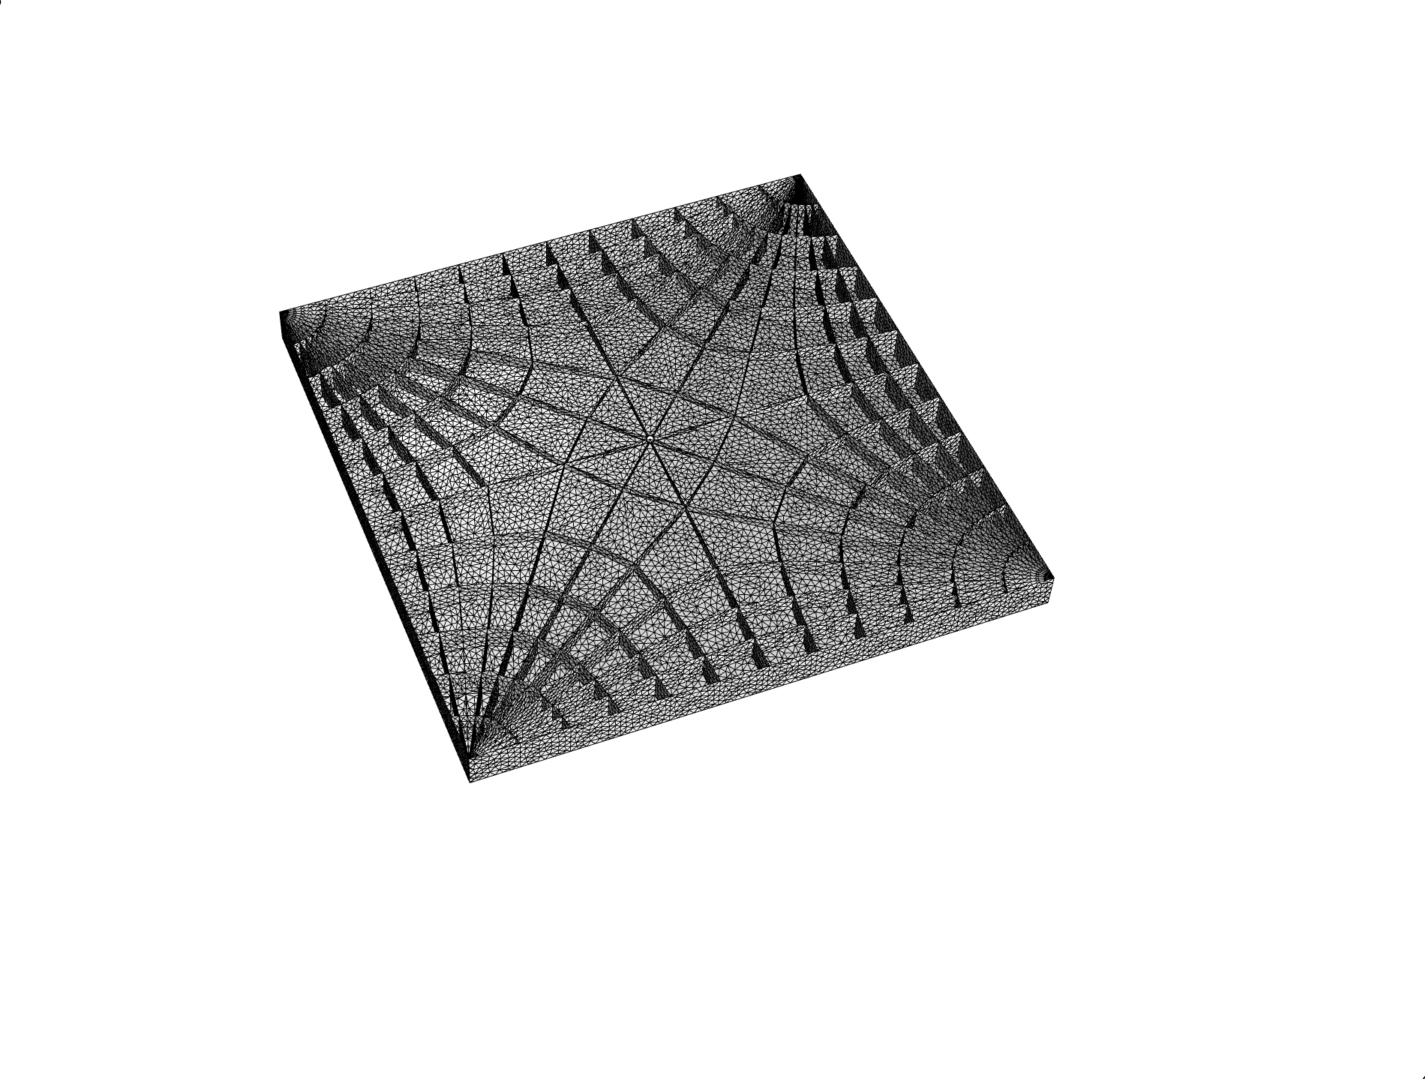
\includegraphics[width=.95\linewidth]{span6}
  \caption{span=6m}
\end{subfigure}

\begin{subfigure}[b]{.48\textwidth}
  \centering
  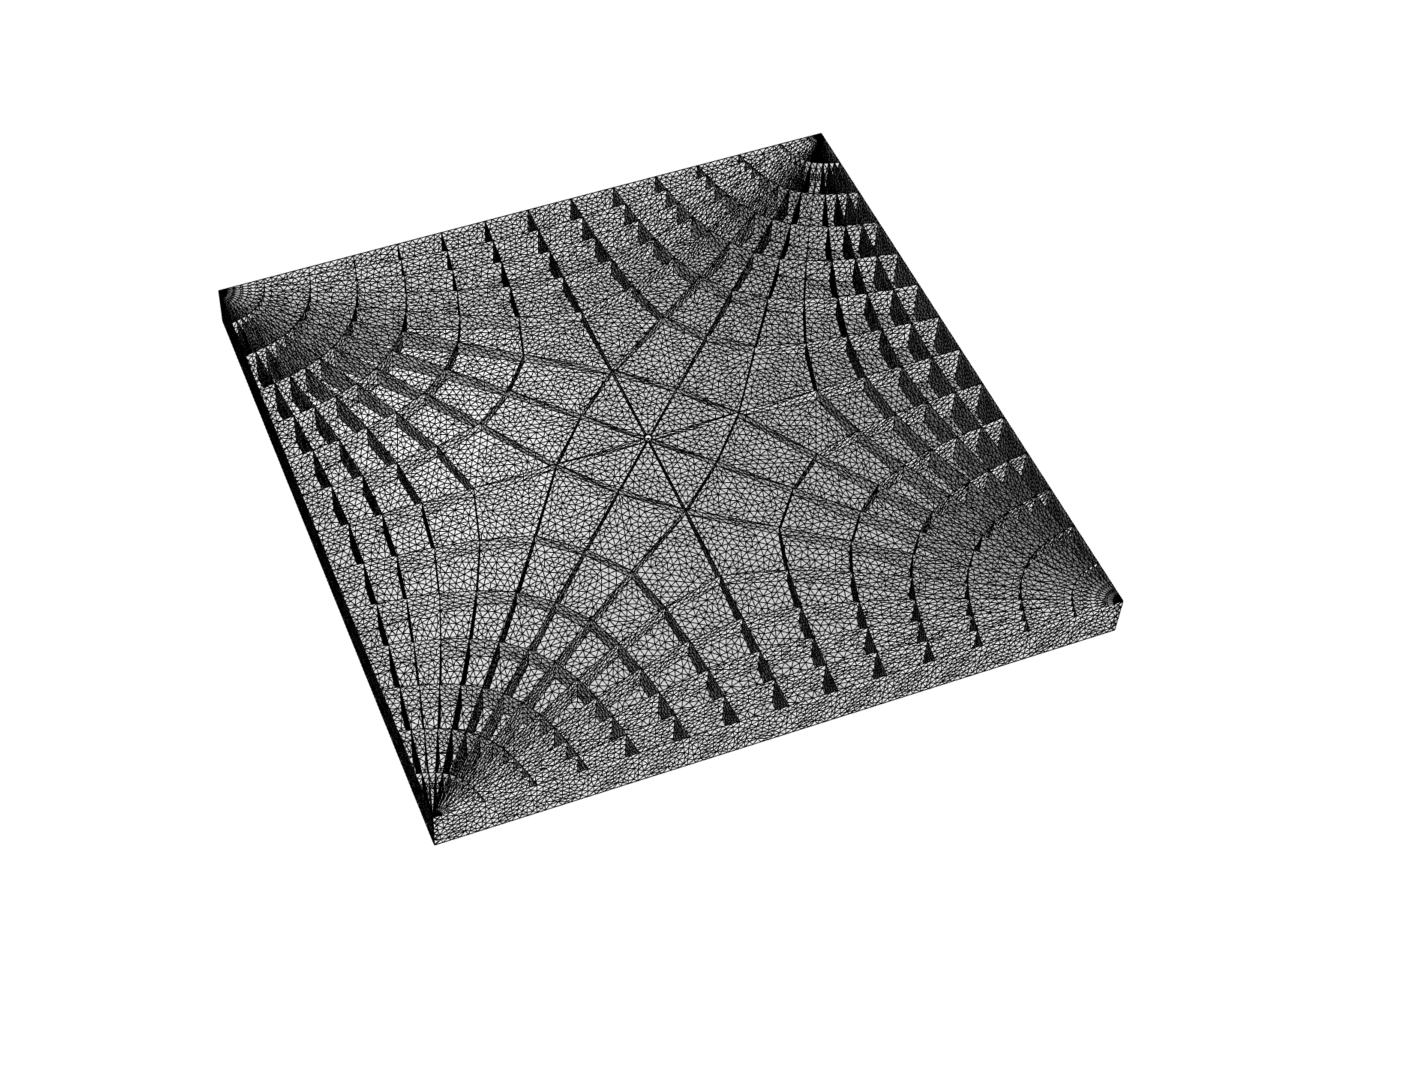
\includegraphics[width=.95\linewidth]{span7}
  \caption{span=7m}
\end{subfigure}
~
\begin{subfigure}[b]{.48\textwidth}
  \centering
  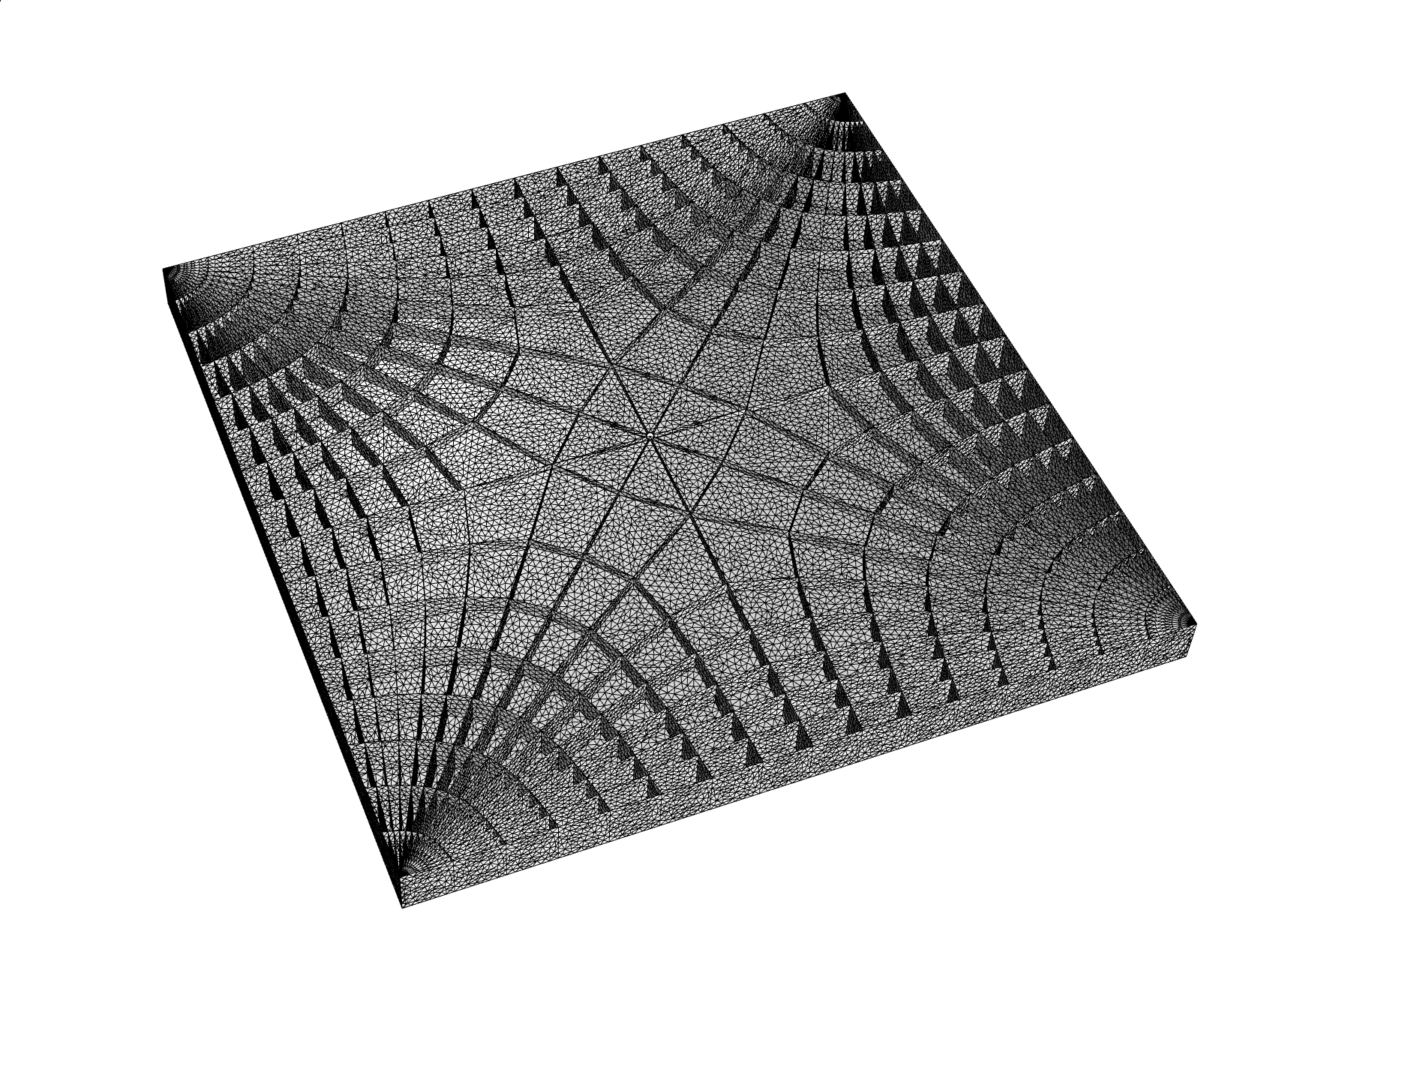
\includegraphics[width=.95\linewidth]{span8}
  \caption{span=8m}
\end{subfigure}

\begin{subfigure}[b]{.48\textwidth}
  \centering
  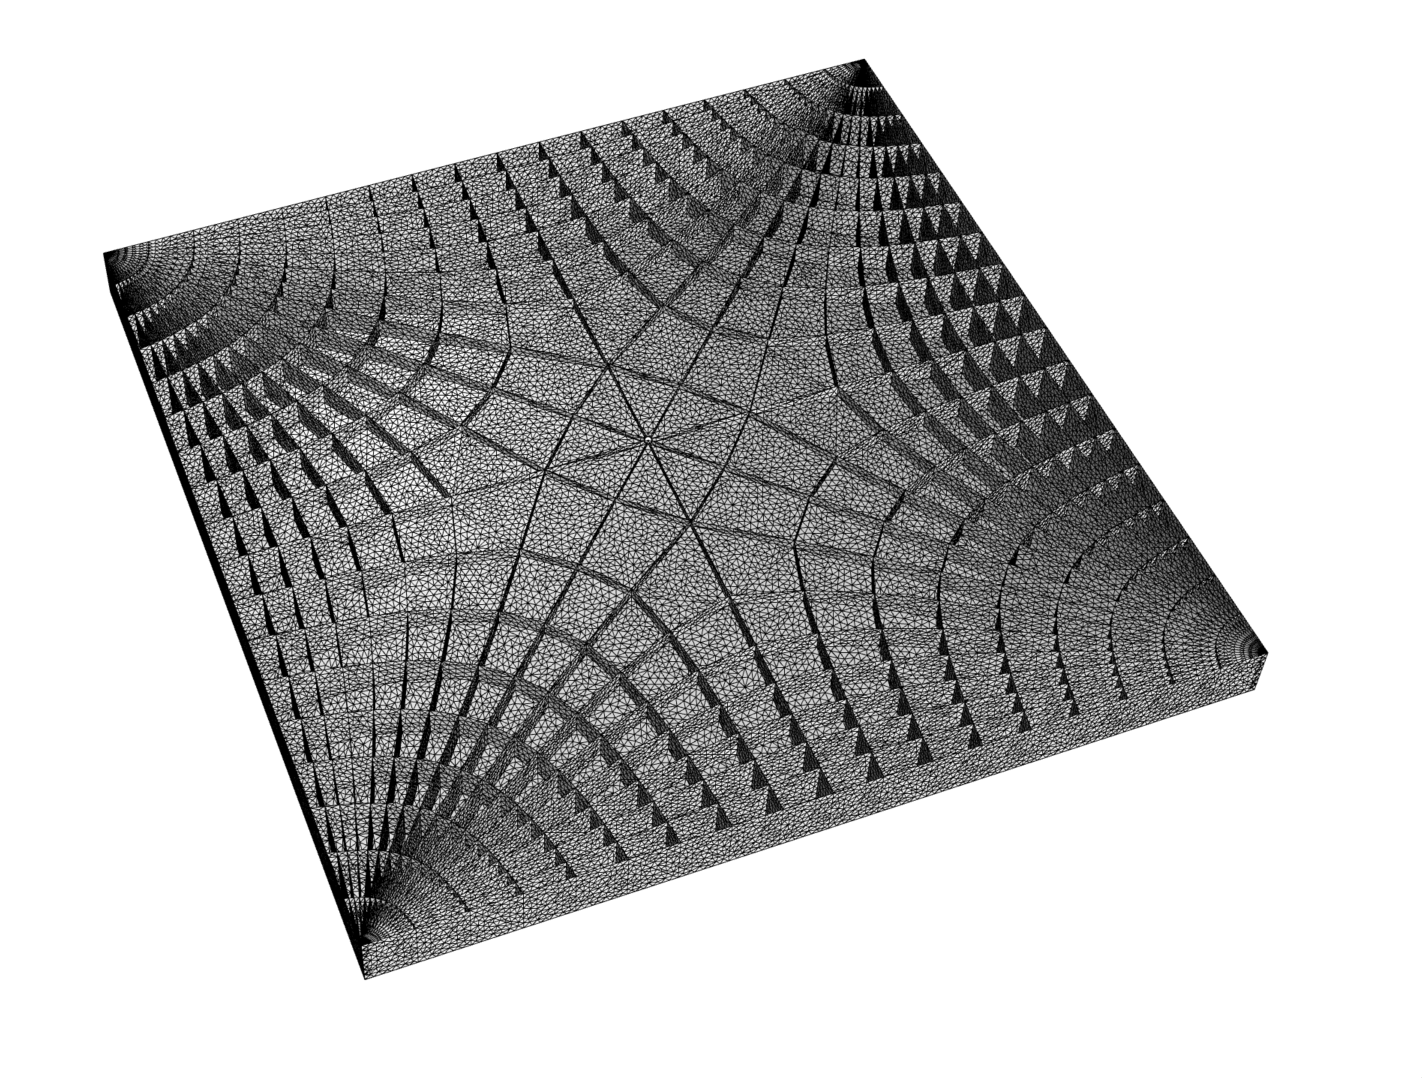
\includegraphics[width=.95\linewidth]{span9}
  \caption{span=9m}
\end{subfigure}
~
\begin{subfigure}[b]{.48\textwidth}
  \centering
  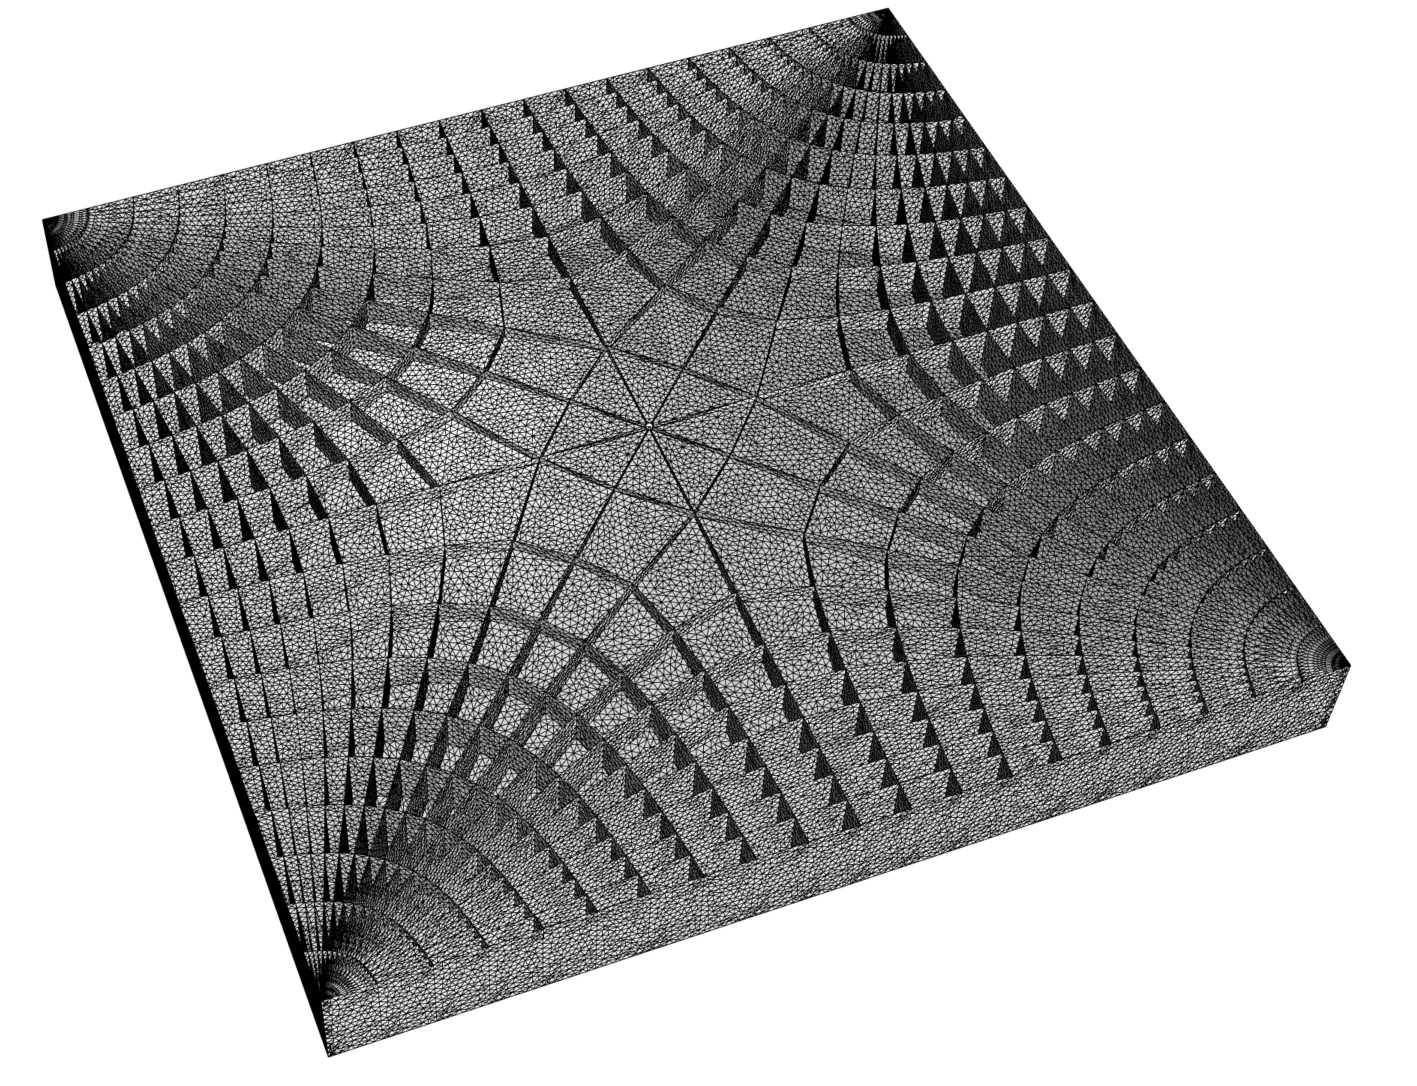
\includegraphics[width=.95\linewidth]{span10}
  \caption{span=10m}
\end{subfigure}

\caption{Mesh models with different spans}
\label{fig:mehs_models}
\end{figure}

\subsection{Material of choice}
The floor will be made of fiber-reinforced concrete. The density and Poisson's ratio are set to be 2400 kg/m$^3$ and 0.2 respectively, the same as common engineering use. The Young's modulus,nevertheless, should take a higher value for a dynamic process. A dynamic Young's modulus of 38 GPa is proposed by SCI P354 for normal weight concrete, irrespective of the actual concrete class. An isotropic elastic behavior of the concrete is assumed for this floor, as the excess of the tensile strength of concrete for such a compression dominate floor is unlikely during human-induced vibration, and the potential anisotropic behavior that may be introduced by rebars in normal reinforced concrete is also excluded here.

\subsection{Structural considerations}
Shell elements will be provided to represent the floor mesh. Given that the floor is considered to be resting without connection constraining rotation on the four supporting edges, these have been considered as lines of pinned nodes, as in vibration the strains are not large enough to overcome the friction \cite{smith2007design}, even though the floor may have roller boundary conditions for static cases. The structural frame that would support the floor element in the construction setting is not considered as part of the modeling. A damping ratio of 3\% is assumed for fully fitted out and furnished floors in normal use \cite{smith2007design}. The beneficial influence of office partitions on the stiffness and additional masses of furniture and finishing is conservatively not considered.

\subsection{Footfall loading}
The excitation point and response point should be chosen to produce the maximum response of the floor. In most cases the two points will represent the same point. Theoretically, it should be checked for every point defined in the finite element analysis. In practice, however, only the points that correspond to the maximum amplitudes for each mode need to be checked \cite{smith2007design}. As the first mode whose vibration shape has its peak in the middle dominates the response, the footfall excitation is presumed to act on the middle point of the floor. 

Continuous footfall excitation is uncommon, but it is representative of the worst possible loading scenario for a given forcing function. The forcing function from a walking activity is assumed to perfectly periodic and can be represented by the sum of four harmonic Fourier series in time history:
\begin{equation}
P(t)=W\left[1+\sum_h\alpha_h \sin(2\pi h f_\mathrm{p} t + \phi_h)\right]
\label{eqn:footfall_SCI}
\end{equation}
where:\par
\makebox[1.5cm]{$W$}  is the weight of an average person\par
\makebox[1.5cm]{$h$}  is the harmonic mode number\par
\makebox[1.5cm]{$\alpha_h$} is the dynamic coefficient for mode $h$\par
\makebox[1.5cm]{$f_\mathrm{p}$} is the pacing frequency\par
\makebox[1.5cm]{$\phi_h$} is the phase angle\par
\noindent
These Fourier coefficients can be extracted from table \ref{tab:fourier coeff}.

{
\renewcommand{\arraystretch}{1.2}
\begin{table}[H]
\centering
\caption{Fourier coefficients for walking activities}
\label{tab:fourier coeff}
\begin{tabular}{cccc}
\Xhline{2\arrayrulewidth}
\textbf{harmonic} & \textbf{pace frequency} & \textbf{dynamic coefficient} & \textbf{phase angle} \\
$\boldsymbol{h}$    & $\boldsymbol{hf_p}$ \textbf{(Hz)}  & $\boldsymbol{\alpha_h}$        & $\boldsymbol{\phi_h}$ \\ \Xhline{2\arrayrulewidth}
1                 & 1.8 to 2.2              & 0.436($hf_p$-0.95)           & 0                    \\
2                 & 3.6 to 4.4              & 0.006($hf_p$+12.3)           & $-\pi/2$                    \\
3                 & 5.4 to 6.6              & 0.007($hf_p$+5.2)            & $\pi$                    \\
4                 & 7.2 to 8.8              & 0.007($hf_p$+2.0)            & $\pi/2$                    \\ \Xhline{2\arrayrulewidth}
\end{tabular}
\end{table}
}
\noindent
A pace frequency of 2 Hz is adopted for analysis, figure \ref{fig:footfall} plots the footfall load time history for one walking cycle (two pace periods, 1 second). The peak value can be ca. 70\% higher than the average.
\begin{figure}[H]
\centering
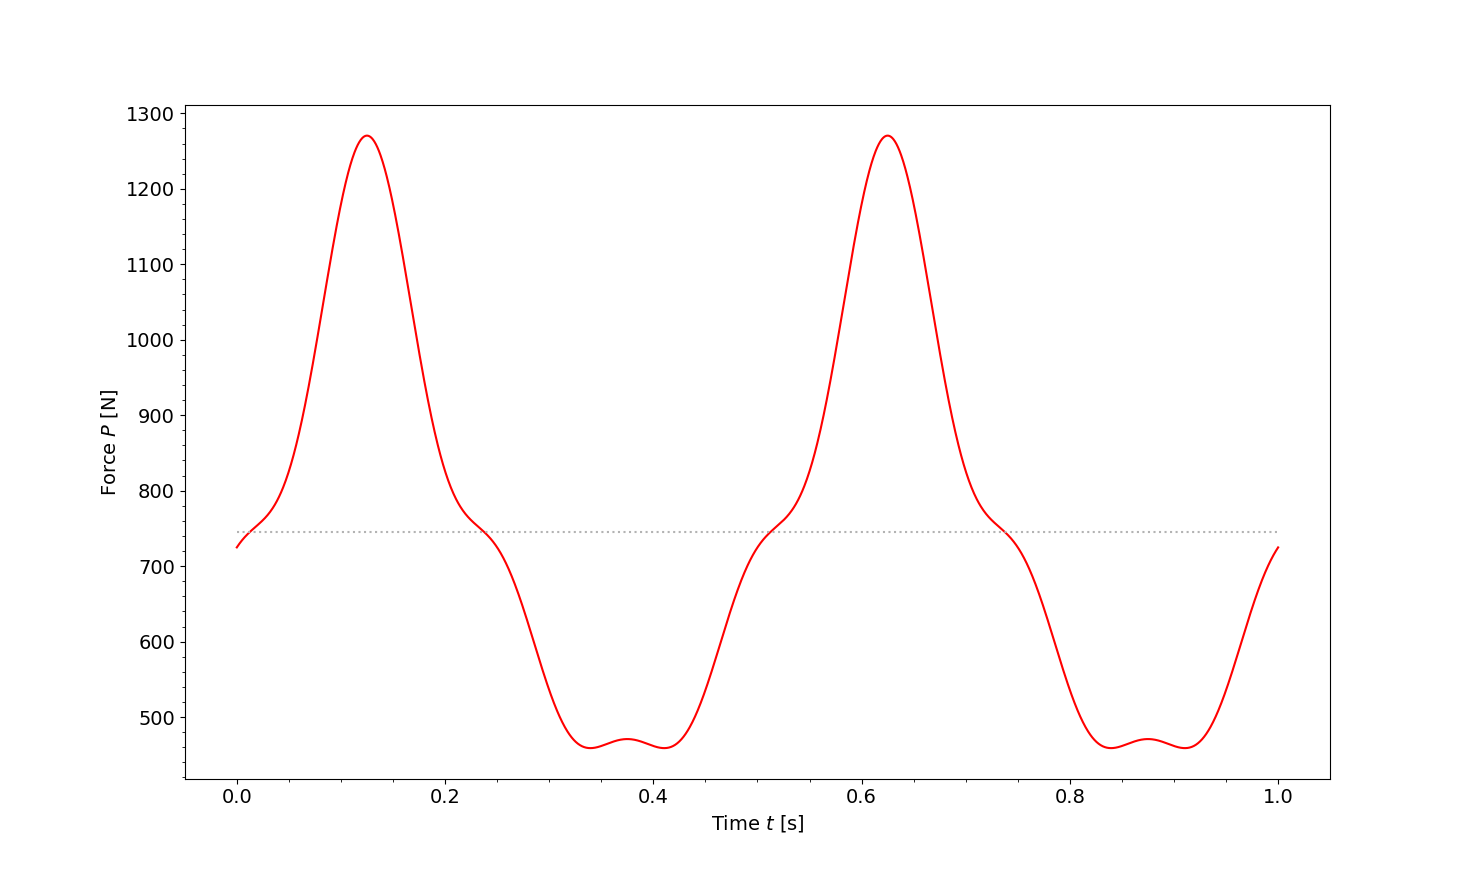
\includegraphics[width=1.0\textwidth]{images/footfall}
\caption{Footfall loading for one walking cycle}
\label{fig:footfall}
\end{figure}

\section{Solution of dynamic response}
\subsection{Theoretical background of modal superposition}
\label{subsec:modal_superposition}
 The equation of motion for a MDOF (multi-degree of freedom) system with damping is
\begin{equation}
\mathbf{m\ddot{u}}+\mathbf{c\dot{u}}+\mathbf{ku}=\mathbf{P}
\label{eqn:motion}
\end{equation}
\noindent
where the square matrices $\textbf{m}$, $\textbf{k}$ and $\textbf{c}$ represent mass, stiffness and damping of the system.

A direct solution of this equation set might be seriously impeded by coupled unknowns, as in normal cases the stiffness matrix $\textbf{k}$ and damping matrix $\textbf{c}$ have off-diagonal terms. The simultaneous solution of these coupled equations is generally not efficient, especially with large amount of DOFs. An alternative is to expand the displacement vector $\mathbf{u}$ of the MDOF system in terms of modal contributions expressed as
\begin{equation}
\mathbf{u}(t)=\sum_{n=1}^N\mathbf{u}_n(t)=\sum_{n=1}^N\boldsymbol{\phi}_nq_n(t)
\label{eqn:u}
\end{equation}
\noindent
where $\boldsymbol{\phi}_n$ is the mode shape and $q_n(t)$ is the associated modal coordinate. Observe that the vibration of each mode is decomposed into two parts, the mode shape that characterizes the vibration pattern along DOFs and keeps invariant to time, the modal coordinate that represents the amplitude of vibration along time points and keeps unchanged for each DOF.  

Using equation \ref{eqn:u}, the coupled equations (\ref{eqn:motion}) can be transformed to a set of uncoupled equations with modal coordinates $q_n(t)$ as the unknowns \cite{chopra2007dynamics}. The equation governs the $n$th modal coordinate $q_n(t)$ reads
\begin{equation}
\ddot{q_n}+2\xi_n\omega_n\dot{q_n}+\omega_n^2q_n=P_n(t)
\label{eqn:motion_q}
\end{equation}
\noindent   
where $\xi_n$ represents the modal damping ratio, $\omega_n$ the angular frequency, $P_n(t)$ the modal load. 

To solve equation \ref{eqn:motion_q}, modal analysis needs to be conducted as the first step for mode shape $\boldsymbol{\phi}_n$ and angular frequency $\omega_n$. They are inherent characteristics of a structure obtained by solving the matrix eigenvalue problem
\begin{equation}
\label{eqn:eigenvalue}
    \left[\textbf{k}-\omega_n^2\textbf{m}\right]\boldsymbol{\phi}_n=\textbf{0}
\end{equation}
\noindent
This equation will have non-trivial solutions only when
\begin{equation}
\label{eqn:eigenvalue_det}
    \text{det}[\textbf{k}-\omega_n^2\textbf m]=0
\end{equation}
\noindent
Through this equation $\omega_n$ can be solved, then substitute the solution in equation \ref{eqn:eigenvalue} to calculate $\boldsymbol{\phi}_n$. Note that the mode shape could be scaled arbitrarily, in this research it is so normalized that the maximum item in each mode is equal to 1. Another modal parameter, modal mass $m_n$, is calculated by
\begin{equation}
\label{eqn:mn}
    m_n = \boldsymbol{\phi}_n^T\textbf{m}\boldsymbol{\phi}_n
\end{equation}

\subsection{Modal analysis}
The mesh models in Rhino, together with information about material, section properties, boundary conditions, the load poin are exported to Abaqus. Abaqus assembles these shell elements and generates the mass matrix and stiffness matrix. The calculation of  modal parameters is based on equation \ref{eqn:eigenvalue} to \ref{eqn:mn}. Figure \ref{fig:mode_shapes} shows the first 4 unique modes (some modes are repeated because of symmetry) of the floor for quick check of the plausibility.
\begin{figure}[H]
\begin{subfigure}[b]{.48\textwidth}
  \centering
  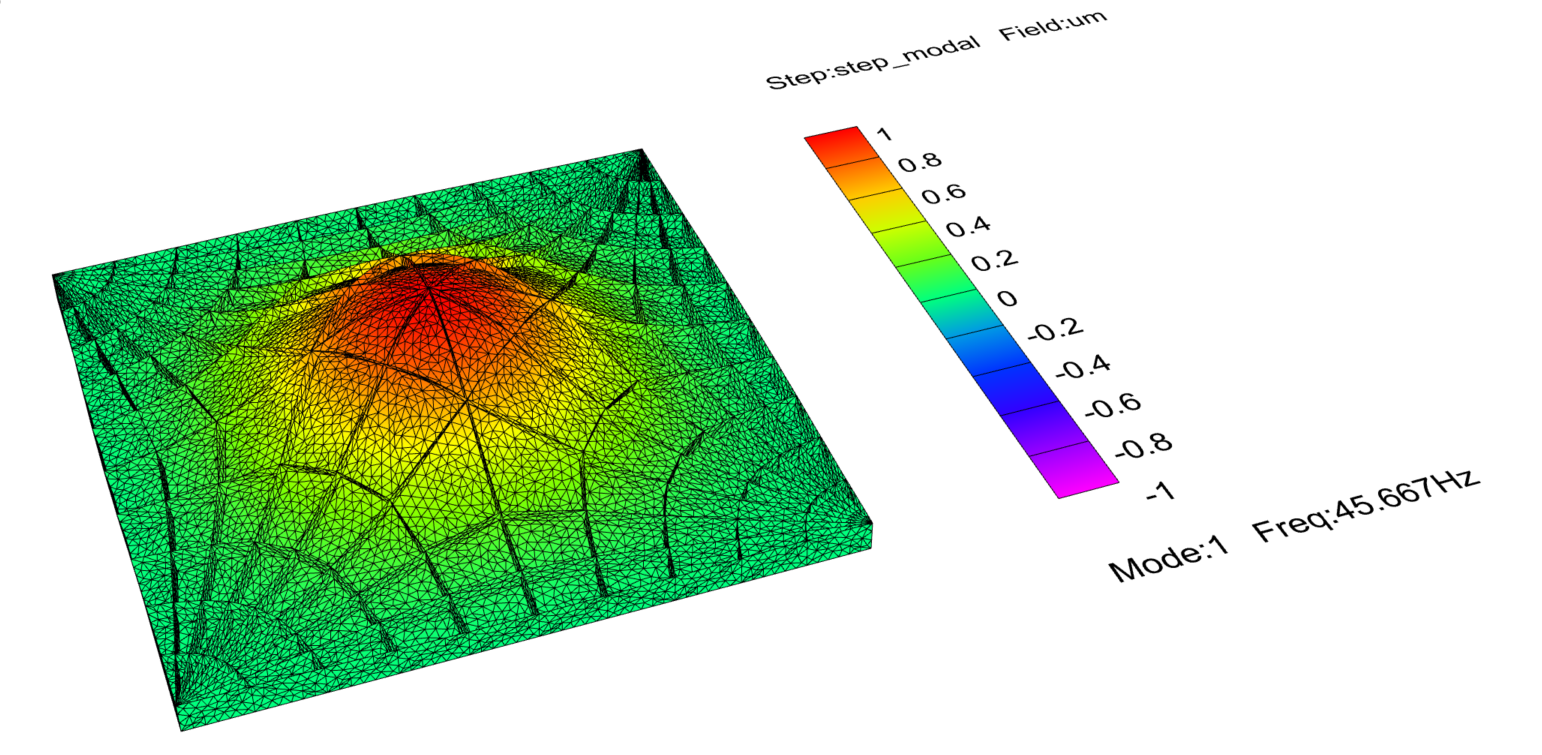
\includegraphics[width=.95\linewidth]{mode1}
  \caption{1st mode}
\end{subfigure}
~
\begin{subfigure}[b]{.48\textwidth}
  \centering
  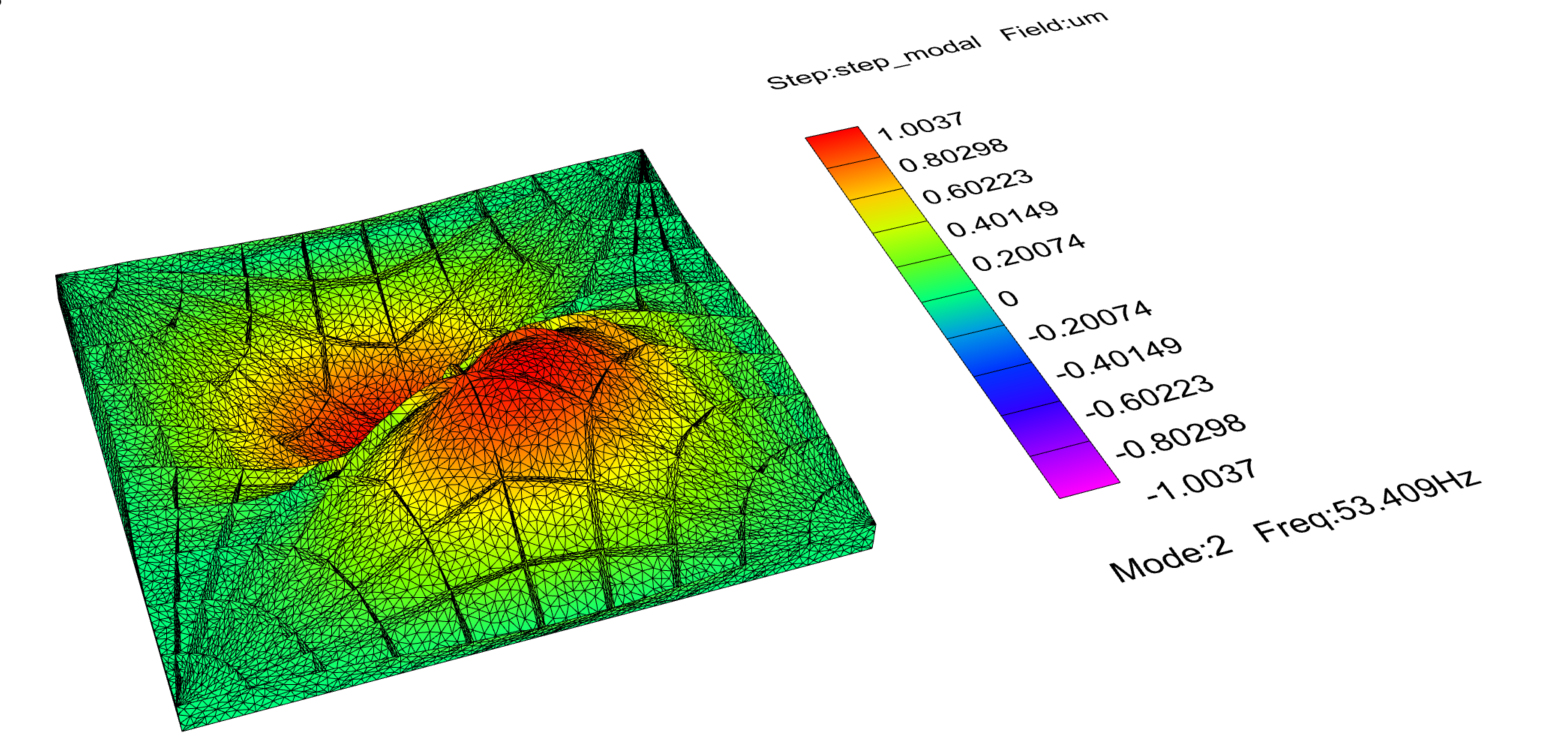
\includegraphics[width=.95\linewidth]{mode2}
  \caption{2nd mode}
\end{subfigure}

\begin{subfigure}[b]{.48\textwidth}
  \centering
  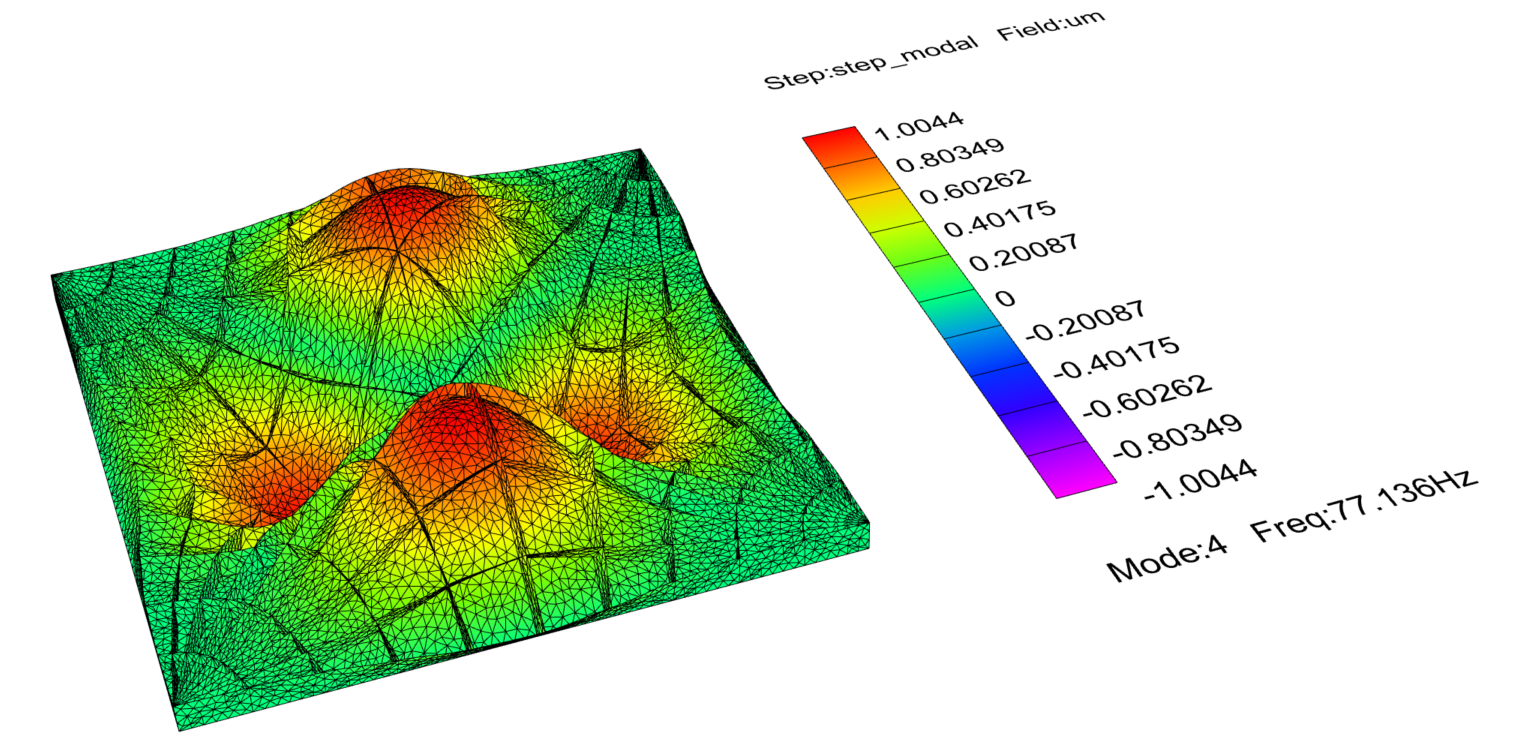
\includegraphics[width=.95\linewidth]{mode4}
  \caption{4th mode}
\end{subfigure}
~
\begin{subfigure}[b]{.48\textwidth}
  \centering
  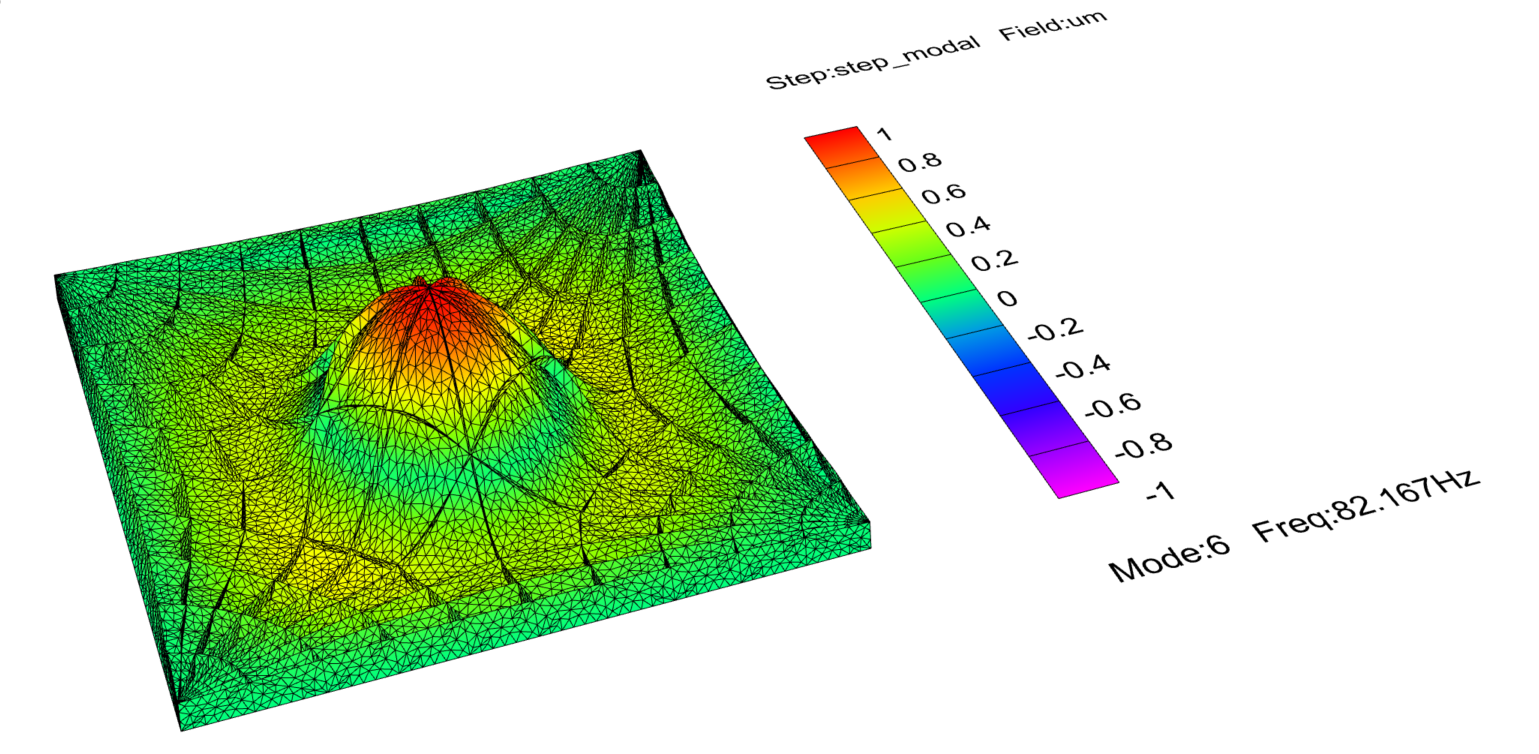
\includegraphics[width=.95\linewidth]{mode6}
  \caption{6th mode}
\end{subfigure}

\caption{The first 4 unique modes of floor with $l=5m, l/d=20, t_v/t_r=1$}
\label{fig:mode_shapes}
\end{figure}


\subsection{Response time history}
\label{subsec:resp_time_histroy}
Since the mode shapes are already available, the next step is to solve the modal coordinates $q_n(t)$ that vary wit time. In equation \ref{eqn:motion_q}, the modal load $P_n(t)$ can be calculated as follows:
\begin{enumerate}
    \item 
     Express the external load $\textbf{P}$(\textbf{s},t) acting on the MDOF system in terms of spatial distribution $\mathbf{s}$ and time variation $P(t)$: 
    \begin{equation}
    \mathbf{P}(\mathbf{s},t)=\mathbf{s}P(t)
    \end{equation}
    \noindent
    where spatical distribution \textbf{s} is a vector of size the number of DOFs in the system, with representative value in position whose corresponding DOF is loaded, and with 0 if not loaded. Time variation $P(t)$ can be the footfall loading expressed in equation \ref{eqn:footfall_SCI}. 

    \item
    Calculate the modal participation factor 
    \begin{equation}
    \label{eqn:Gamma}
    \Gamma_n=\frac{\boldsymbol{\phi}_n^T\mathbf{s}}{M_n}
    \end{equation}
    
    \item
    Then modal load
    \begin{equation}
    P_n(t)=\Gamma_nP(t)
    \end{equation}
\end{enumerate}

Once the modal load is obtained, the second order, ordinary differential equation (\ref{eqn:motion_q}) can be reformed into two first order, ordinary differential equations, expressed in matrix form
\begin{equation}
\begin{bmatrix} \dot{q_n}\\ \ddot{q_n} \end{bmatrix} 
=\begin{bmatrix} 0 & 1 \\ -\omega_n^2 & -2\xi_n\omega_n \end{bmatrix}
\begin{bmatrix} q_n\\ \dot{q_n} \end{bmatrix}
+ \begin{bmatrix} 0\\ P_n(t) \end{bmatrix}
\end{equation}
\noindent
This matrix equation can be solved with the ODE solver \textit{odeint} in the SciPy module.  Two initial conditions at $t=0$ that represent a rest state, initial displacements $q_n(0)=0$ and initial velocity $\dot{q_n}(0)=0$, are assumed. The results of the \textit{odeint} solver are the displacements and velocities in modal coordinates. The accelerations are then calculated by differentiating the velocities with respect to time. Once the modal coordinates $q_n(t)$ have been solved, the total displacements can be obtained via modal superposition expressed in equation (\ref{eqn:u}).

\section{Evaluation of vibration perception}
The evaluation of the dynamic performance is based on the vibration perception of humans, which is characterized by the frequency weighted root-mean-square (RMS) acceleration of the floor under the footfall loading, expressed by 
\begin{equation}
\label{eqn:aw_rms}
    a_{w,rms}(t)=\sqrt{\frac{1}{T}\int_0^Ta_w(t)^2dt}
\end{equation}
\noindent
where $T$ is the period under consideration, taken as $1/f_p$. The frequency weighted total acceleration $a_w(t)$ is found by summing the acceleration responses of each mode
\begin{equation}
    a_w(t)=\sum_{n=1}^Na_{n,w}(t)
\end{equation}
\noindent
The vibration perception of humans is different with varying vibration frequencies. Humans are generally not sensitive to vibrations with too low or too high frequencies, so actual acceleration should be weighted to reflect the perception of humans. Figure \ref{fig:Wb} shows the frequency weighting curve and functions for vertical vibrations recommended by SCI P354. The weighted acceleration then reads
\begin{equation}
    a_{n,w}(t)=W_b(f_n)a_n(t)
\end{equation}
\noindent
where $a_n(t)$ is the actual acceleration in each mode solved by response time history analysis.

\begin{figure}[H]
\begin{subfigure}[H]{.48\textwidth}
  \centering
  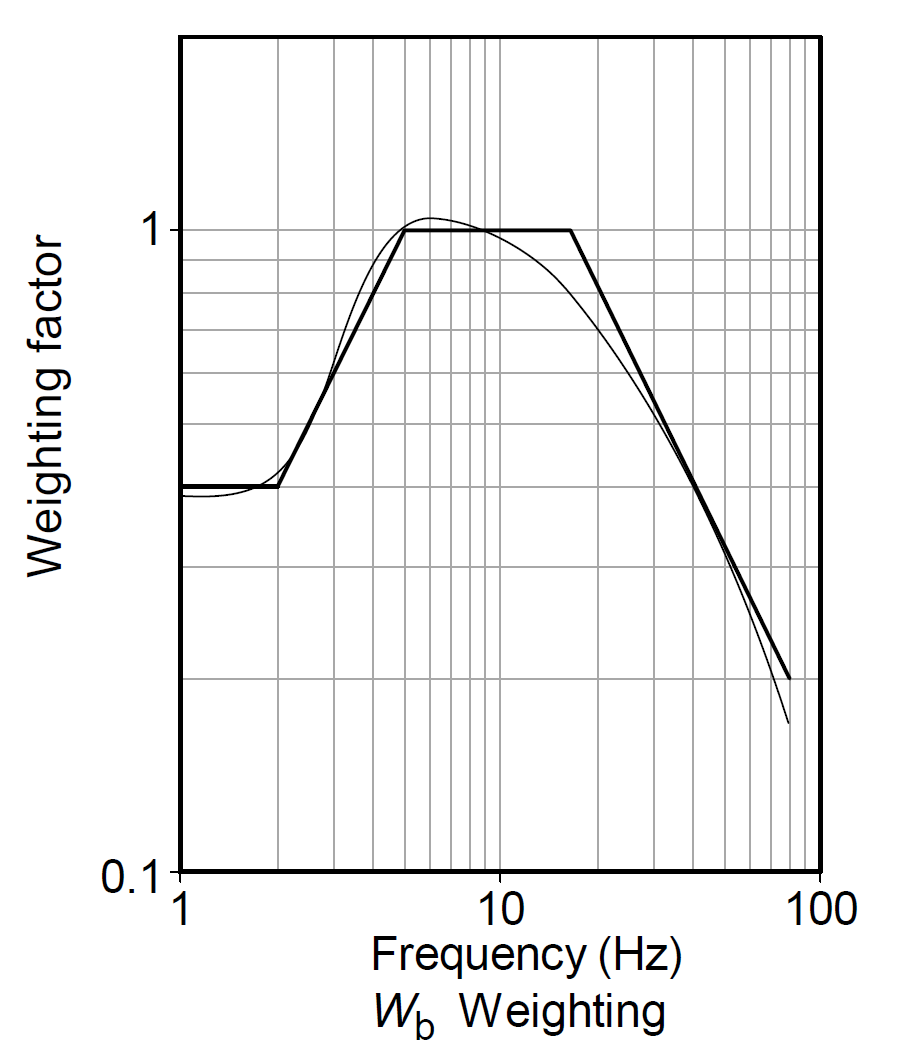
\includegraphics[width=.95\linewidth]{weight_curve}
\end{subfigure}
~
\begin{subfigure}[H]{.5\textwidth}
  \centering
  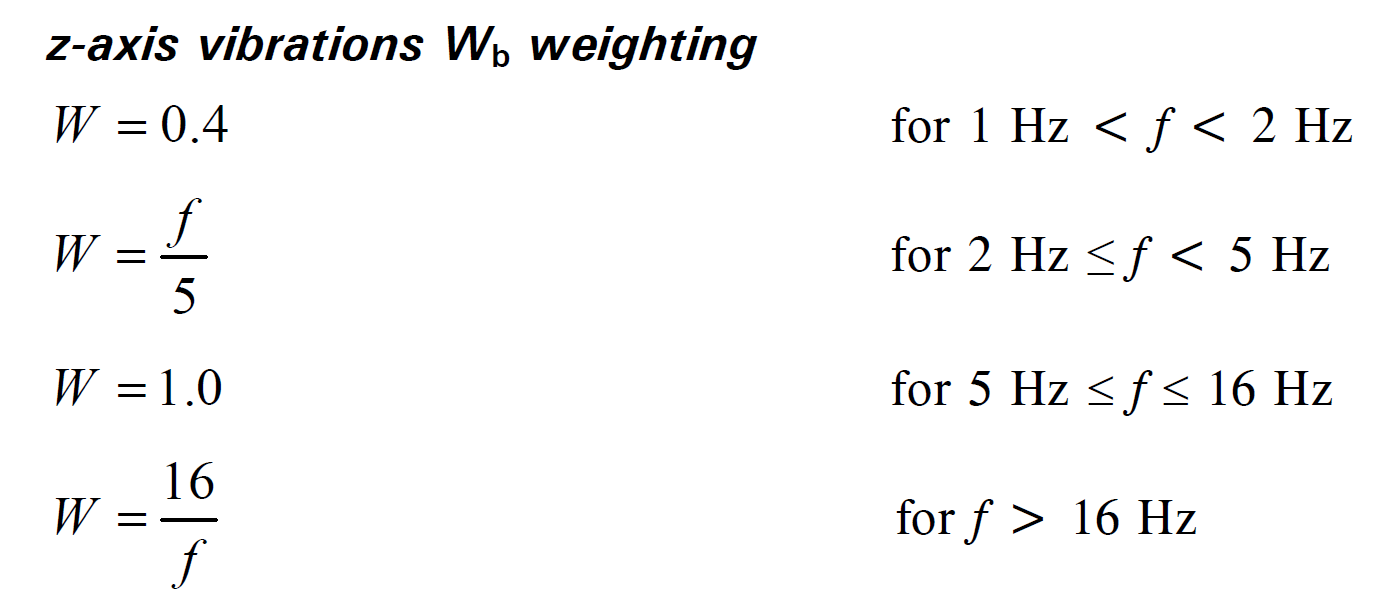
\includegraphics[width=.99\linewidth]{weight_fn}
\end{subfigure}

\caption{Frequency weighting $W_b$}
\label{fig:Wb}
\end{figure}

The next step is to calculate the response factor, which is the ratio between the weighted rms-acceleration $a_{w,rms}$ (peak value) calculated by equation \ref{eqn:aw_rms} and the base value $a_{rms,base}=5\times10^{-3}$ m/s\textsuperscript{2}.

\begin{equation}
    R=\frac{a_{w,rms}}{a_{base,rms}}=\frac{a_{w,rms}}{0.005}
\end{equation}

The response factor should not exceed the recommended multiplying factors listed in table \ref{table:multiplier_SCI}. For office buildings, the maximal response factor is 8, meaning that the allowable weighted rms-acceleration $a_{w,rms,allow}=0.04$\,m/s\textsuperscript{2}.
\begin{table}[H]
\centering
\caption{Recommended multiplying factors based on single person excitation}
\label{table:multiplier_SCI}
\begin{tabular}{c}
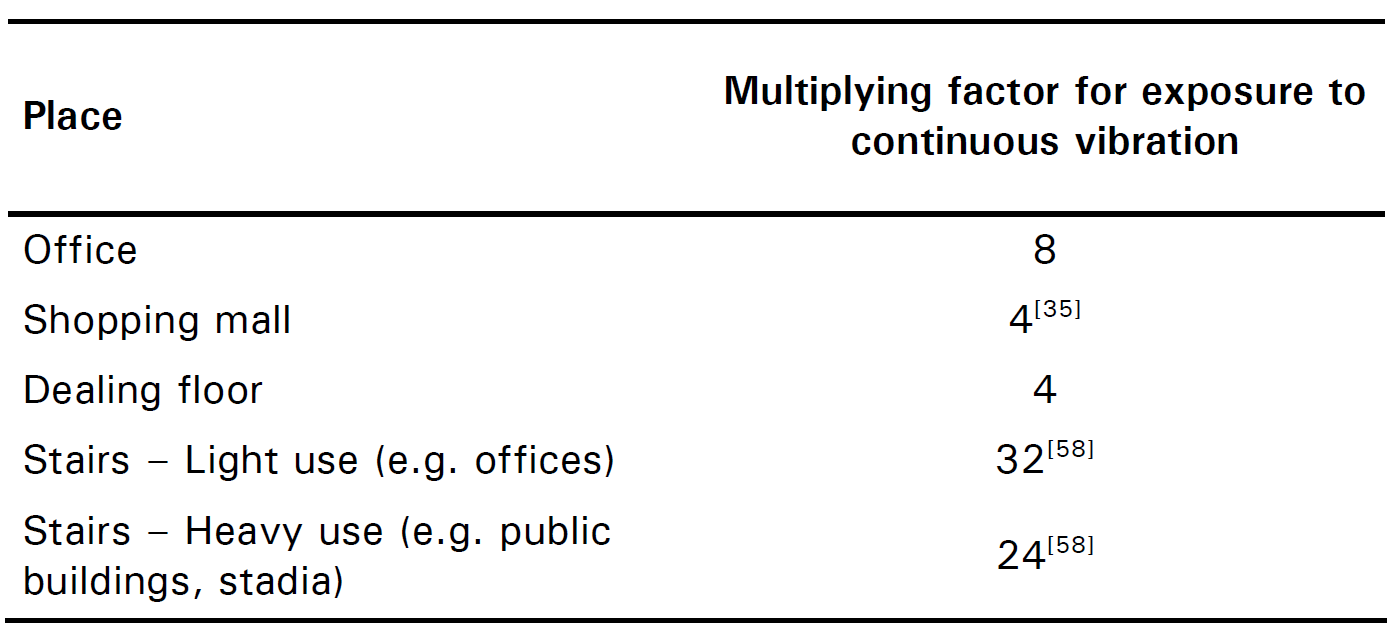
\includegraphics[width=0.7\textwidth]{multiplier_SCI}
\end{tabular}
\end{table}
\chapter{Results of dynamic analysis}
\label{chap4}

\section{Modal analysis}
\label{sec:modal analysis}
Modal masses, natural frequencies and mode shapes are the output of modal analysis, they reflect the dynamic characteristics of the floors. It is meaningful to observe how the input geometric parameters $l, l/d, t_v/t_r$ influence the modal parameters.

To measure the relation between input and output, IOC (input/output correlations) value is introduced. IOC is defined as follows:
\begin{equation}
    IOC_i=\rho_{X_i,Y}=\frac{Cov[X_i,Y]}{\sigma_{X_i}\sigma_Y}
\end{equation}
\noindent
where $\rho$ is Pearson's linear correlation coefficient, $X_i$ is one of the input data sets and $Y$ the output data set, $Cov$ stands for covariance and $\sigma$ the standard deviation. If $|\rho_{X_i,Y}|\approx0$, $X_i$ has no importance. Positive/negative values indicate the increasing/decreasing trend of the mapping $X_i\xrightarrow{}Y$. Although Pearson's correlation coefficient only depicts a linear relationship, it is still applicable for many cases if the relation is not strongly nonlinear.

\subsection{Modal mass}
\label{subsec:modal_mass}

Figure \ref{fig:geom-m1} shows the geometric parameters-modal mass scatter plots with corresponding IOC values. It is evident that the $t_v/t_r$ ratio influences the modal mass most strongly, $l$ less, $l/d$ has almost no importance. The increase of span and more mass on the vault tends to raise the modal mass. The same conclusions can be drawn from figure \ref{fig:l,t-m plot}, in which all information is assembled together, but shown in a less decent way. The modal mass increases in the positive direction of $l$ and $t_v/t_r$ axis. The isolines of different $l/d$ ratios tend to cluster together. The insignificance of $l/d$ ratio is somehow anti-intuitive at the first glance, because if two floors with the same span and thickness ratio are compared, the one with smaller span/depth ratio (higher depth) should have more mass, and hence greater modal mass, but it is not the case. One possible reason is that a floor having a lower $l/d$ value (high depth) can develop a greater arch effect, allowing a less proportion of mass in the middle to vibrate (detailed discussion in the interpretation of figure \ref{fig:geom-m12m} and figure \ref{fig:m12m_change}). The increase of mass because of higher depth and the decrease of modal mass proportion due to stronger arch effect compensate each other to a large extent. 
\begin{figure}[H]
\begin{subfigure}[b]{.32\textwidth}
  \centering
  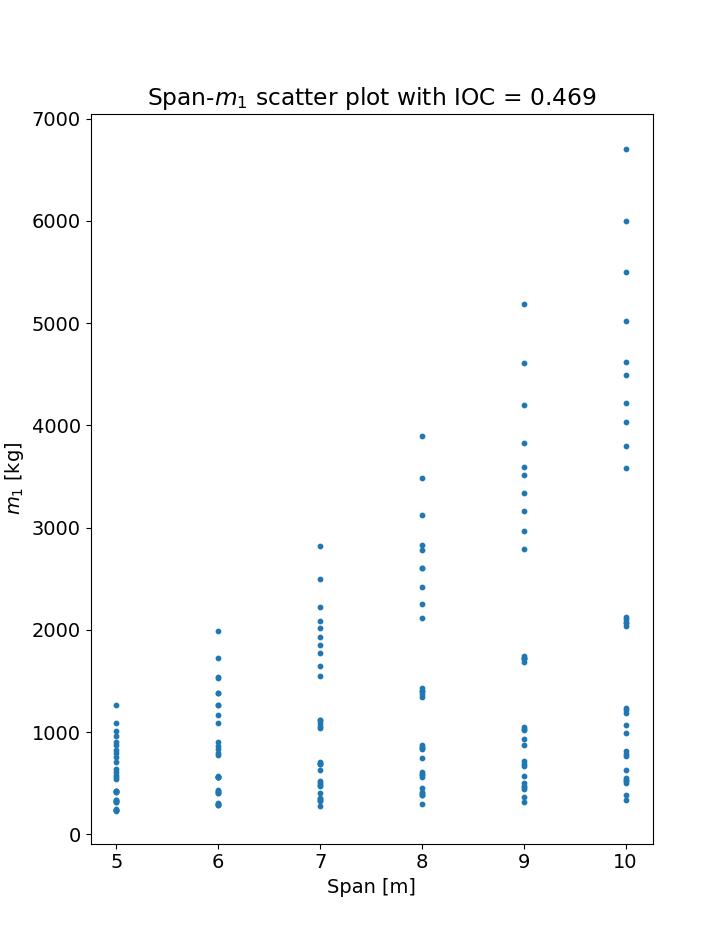
\includegraphics[width=.99\linewidth]{l_m1}
  \caption{$l-m_1$}
\end{subfigure}
~
\begin{subfigure}[b]{.32\textwidth}
  \centering
  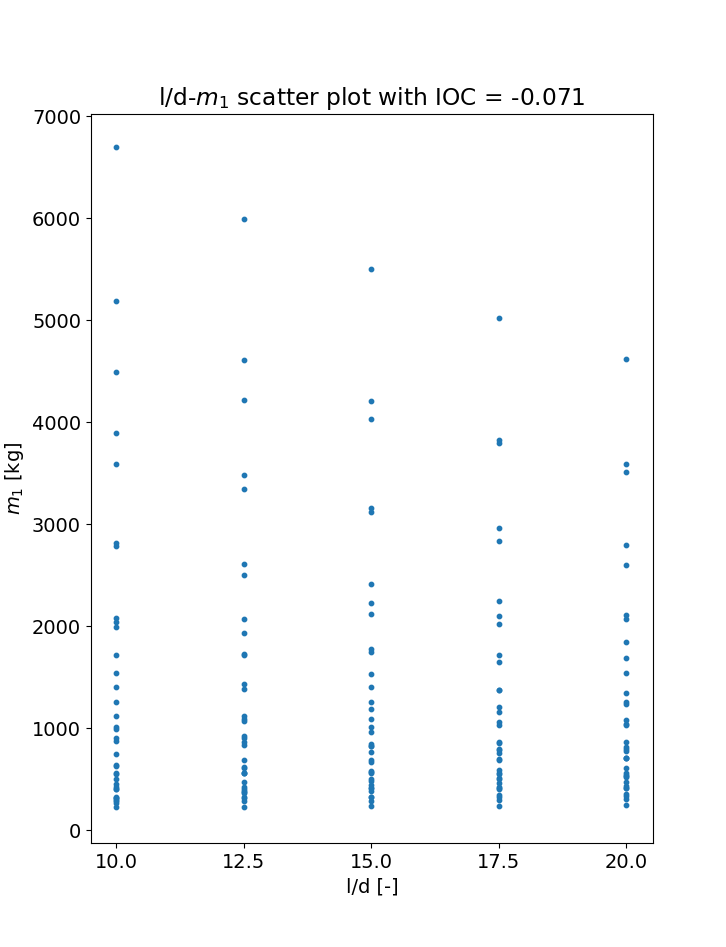
\includegraphics[width=.99\linewidth]{l2d_m1}
  \caption{$l/d-m_1$}
\end{subfigure}
~
\begin{subfigure}[b]{.32\textwidth}
  \centering
  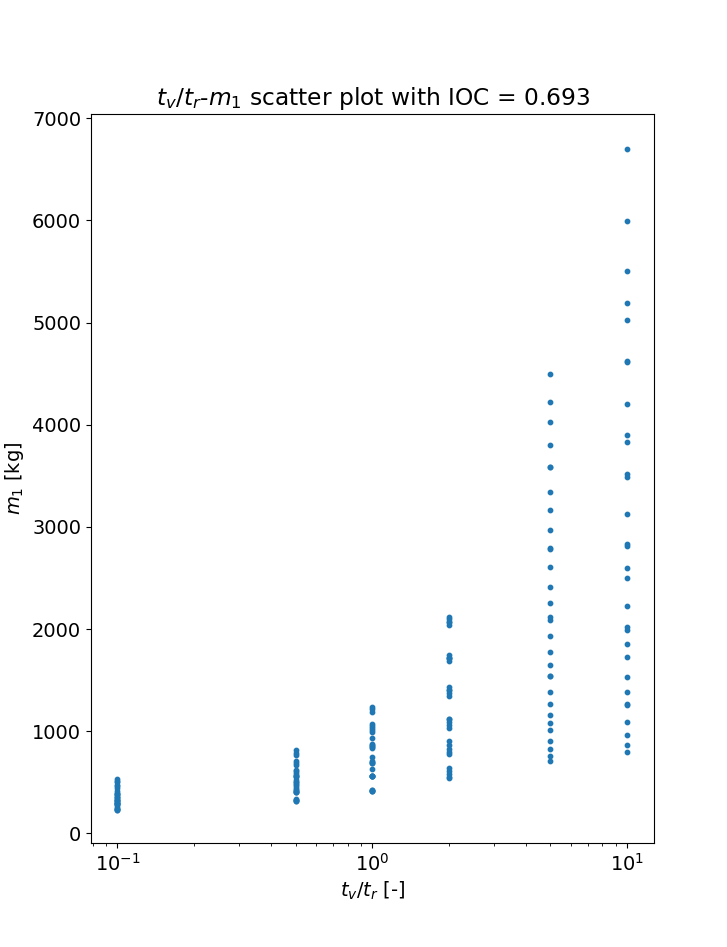
\includegraphics[width=.99\linewidth]{gamma_m1}
  \caption{$t_v/t_r-m_1$}
\end{subfigure}

\caption{Geometric parameters-modal mass (first mode) scatter plot}
\label{fig:geom-m1}
\end{figure}

\begin{figure}[H]
\centering
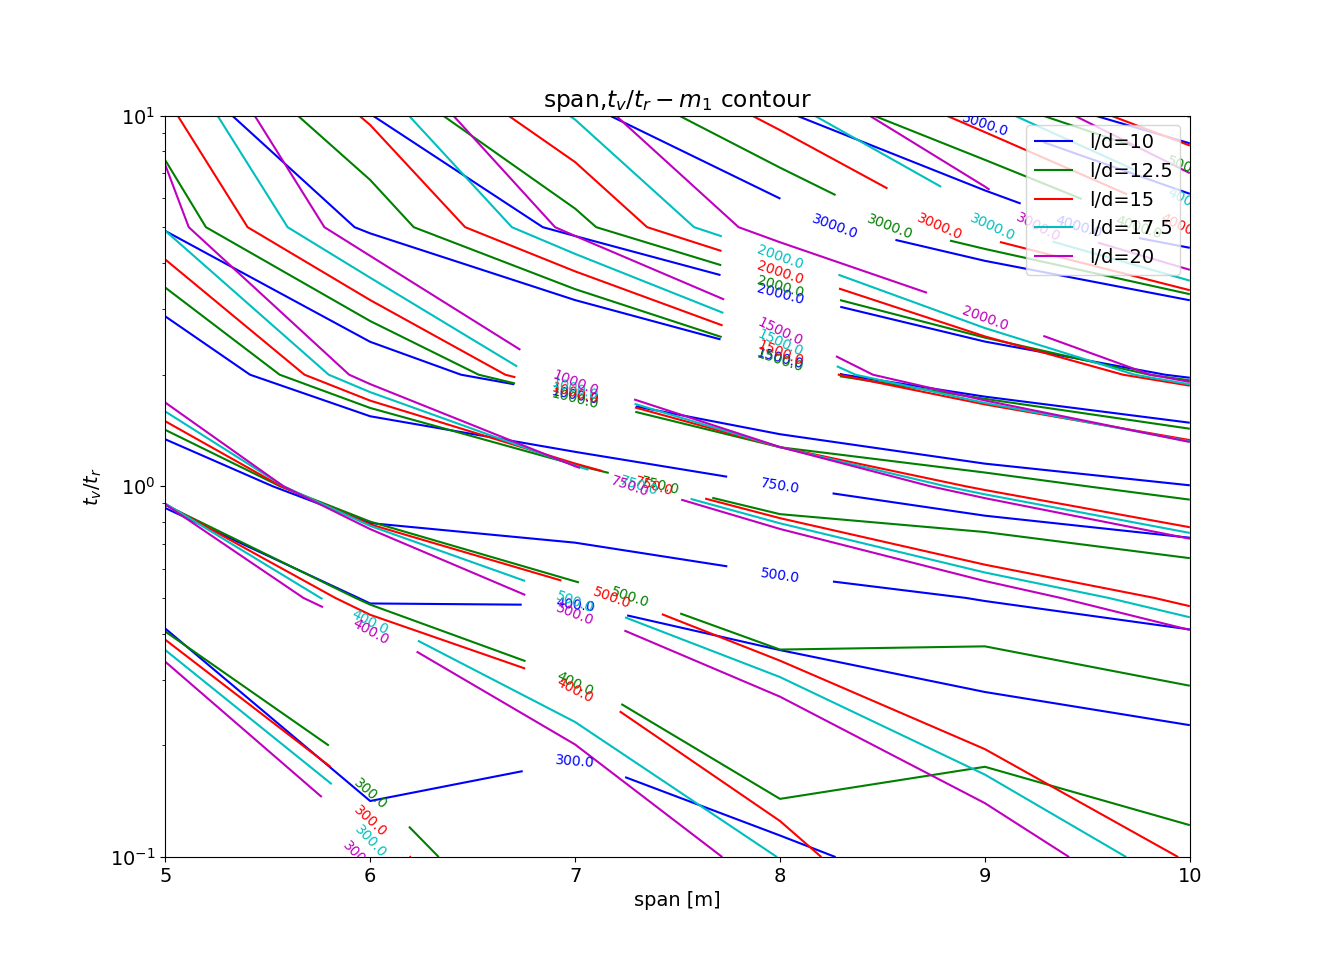
\includegraphics[width=0.9\textwidth]{images/l,gamma-m1.png}
\caption{$l, t_v/t_r - m_1$ contour plot}
\label{fig:l,t-m plot}
\end{figure}

It is interesting to see how the geometry changes the proportion of mass that participates in vibration, namely dimensionless quantity $m_1/m$ (see figure \ref{fig:geom-m12m}). Different from the modal mass, the modal mass proportion decreases with increasing span. It may be explained by the increasing number of ribs near the edges when span raises. The mass proportion of material in the middle becomes less, and the vertical vibration of the floor on the sides is likely to be restricted by the vertically stiff ribs, only allowing a small proportion of mass in the middle to vibrate. With increasing $l/d$ (thinner floor) the modal mass proportion goes up, which is shown more clearly in figure \ref{fig:m12m_change}. This may lie in a weaker arch effect if the vault is too shallow. The extreme is a flat floor without any arch effect leading to a modal mass of 25\% of total mass. The increase of $t_v/t_r$ promotes the modal mass proportion greatly. This is due to different mass and stiffness distribution in the vault and ribs. The vault has a more or less uniform mass distribution over the whole area, whereas the ribs have much higher mass and stiffness concentration around edges allowing only a small proportion of mass in the middle to vibrate. When the two different components work together, the vertically stiff ribs near edges are prone to impose constraints on the vault during vibration. 
No matter how these parameters change, the modal mass proportion can barely reach 13\%, it can be even lower than 0.5\% if ribs dominate. For floors with identical vault and ribs thickness, this value ranges from 1\% to 7\%, compared with flat slab with 25\%, the difference is huge.

\begin{figure}[H]
\begin{subfigure}[b]{.32\textwidth}
  \centering
  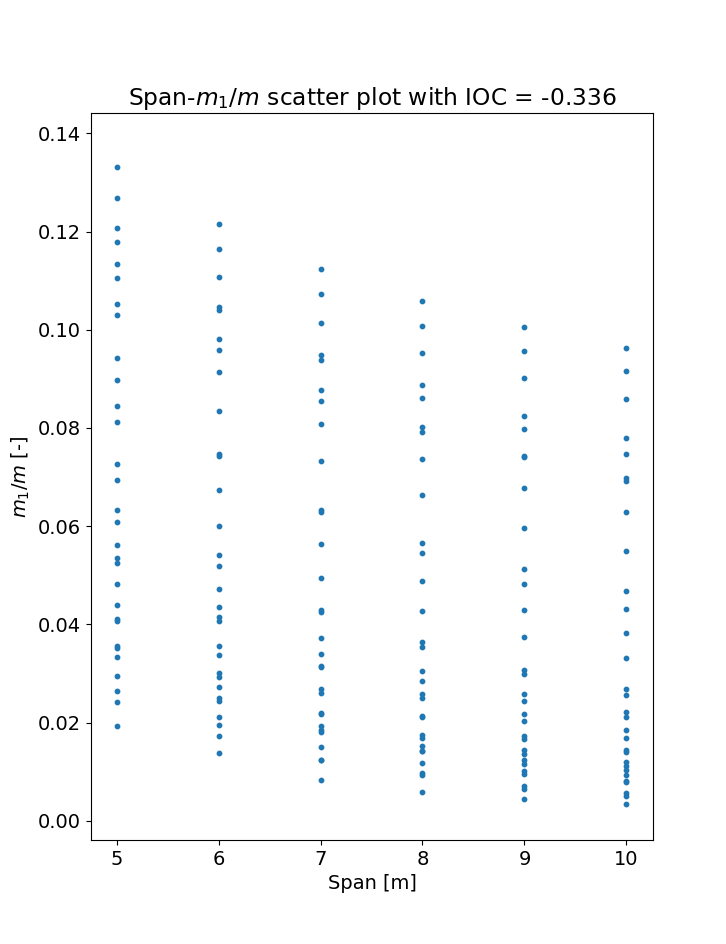
\includegraphics[width=.99\linewidth]{l_m12m}
  \caption{$l-m_1/m$}
\end{subfigure}
~
\begin{subfigure}[b]{.32\textwidth}
  \centering
  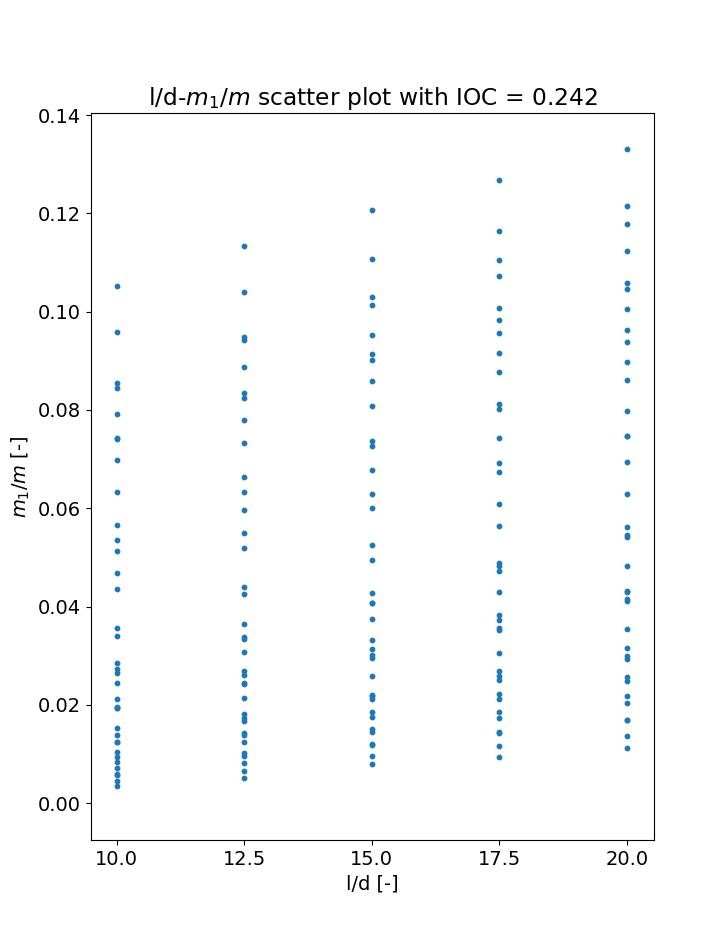
\includegraphics[width=.99\linewidth]{l2d_m12m}
  \caption{$l/d-m_1/m$}
\end{subfigure}
~
\begin{subfigure}[b]{.32\textwidth}
  \centering
  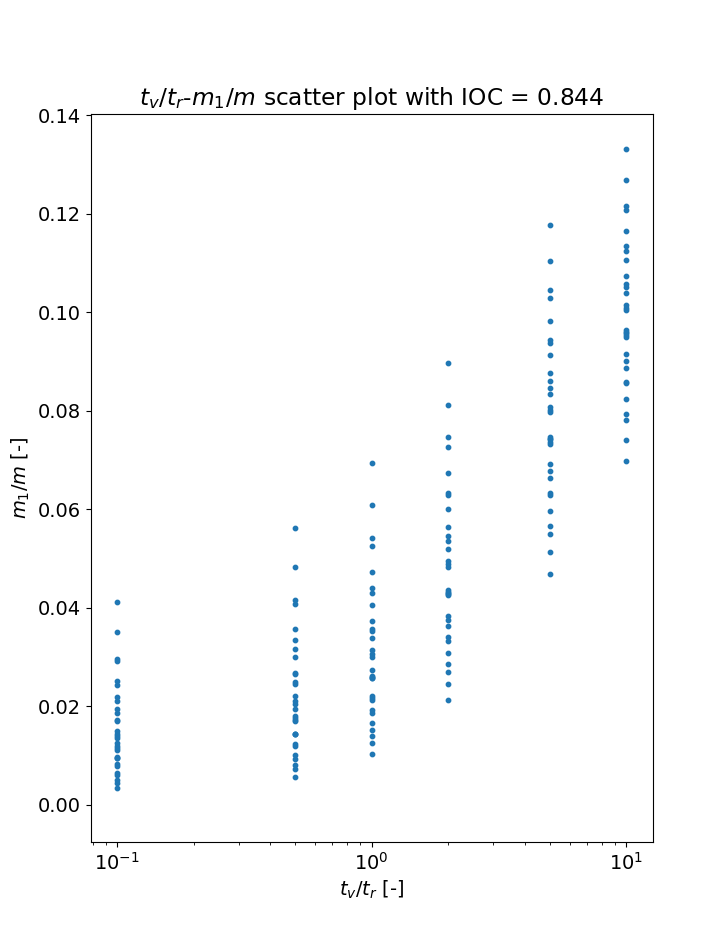
\includegraphics[width=.99\linewidth]{gamma_m12m}
  \caption{$t_v/t_r-m_1/m$}
\end{subfigure}

\caption{Geometric parameters-modal mass (first mode) proportion scatter plot}
\label{fig:geom-m12m}
\end{figure}

\begin{figure}
  \centering
  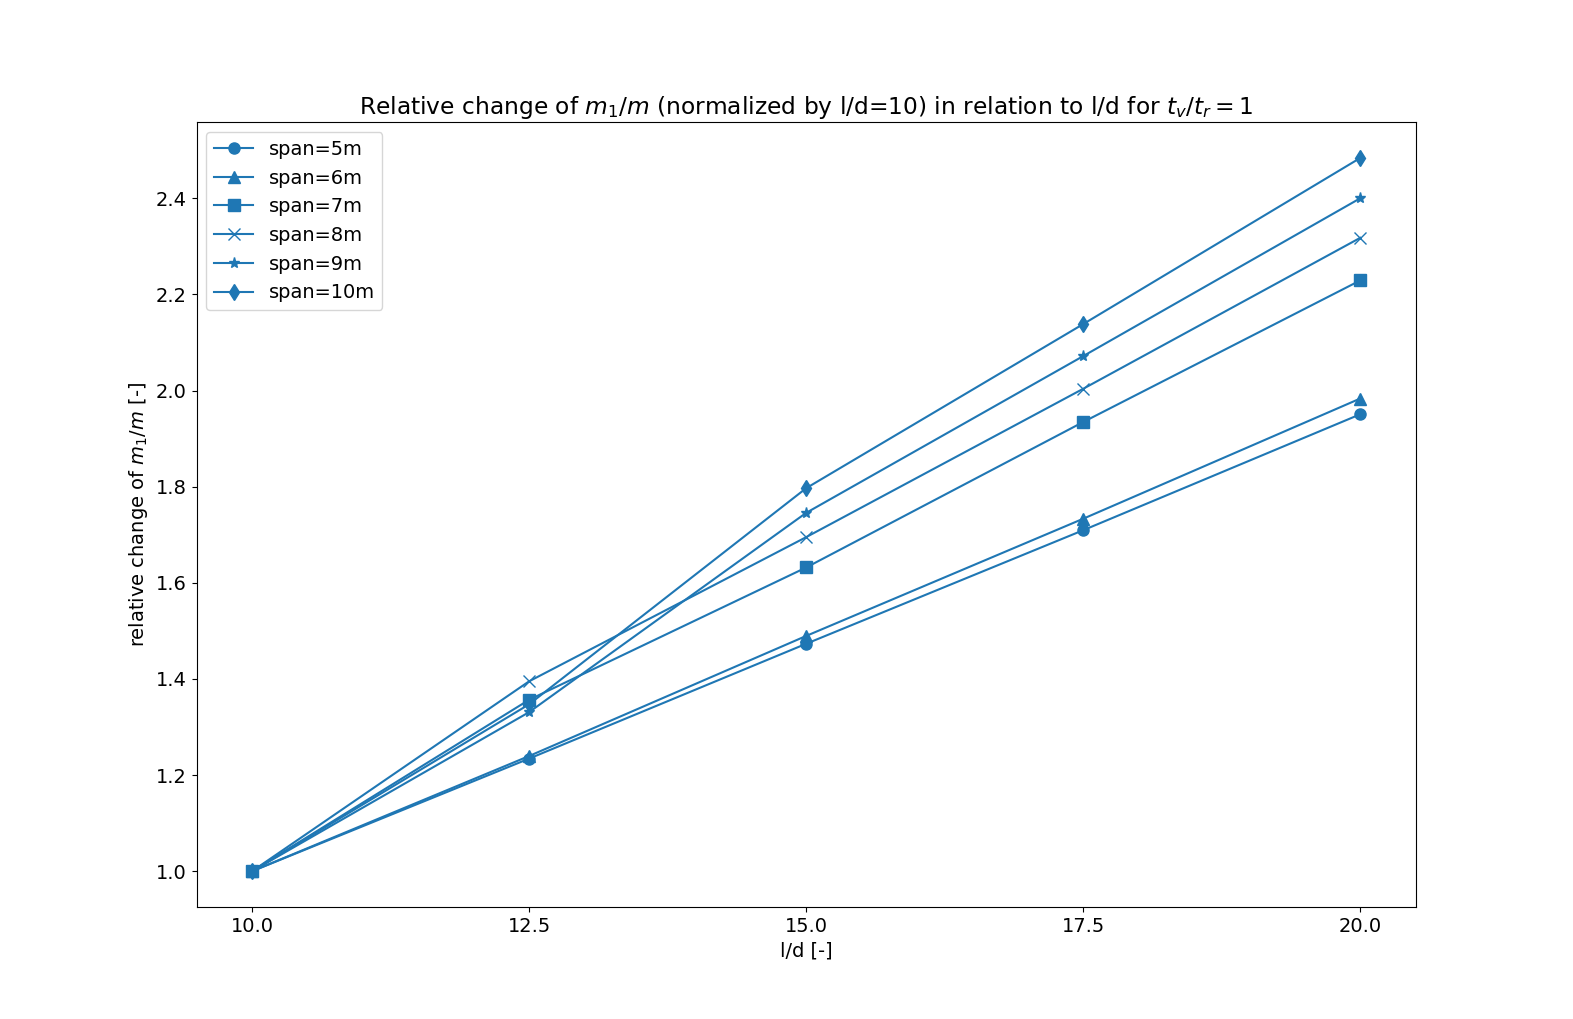
\includegraphics[width=0.9\linewidth]{images/m12m_change}
  \caption{Relative change of $m_1/m$ in relation to l/d}
  \label{fig:m12m_change}
\end{figure}

\subsection{Natural frequency}
\label{subsec:natural frequency}
The relation between natural frequency $f_n$ and angular frequency $\omega_n$ is $f_n=\omega_n/(2\pi)$. It is an important quantify for both low frequency floor as well as high frequency floor. For low frequency floor,it may be associated with the resonant behavior. For high frequency floor, it is the frequency at which the floor vibrates in the transient phase, instead of vibrating at the excitation frequency in the steady phase. The natural frequency is also involved in evaluation of vibration perception by the frequency weighting function. Figure \ref{fig:geom-f1} illustrates how $l, l/d, t_v/t_r$ influences the fundamental frequency (the first natural frequency). 
\begin{figure}[H]
\begin{subfigure}[b]{.32\textwidth}
  \centering
  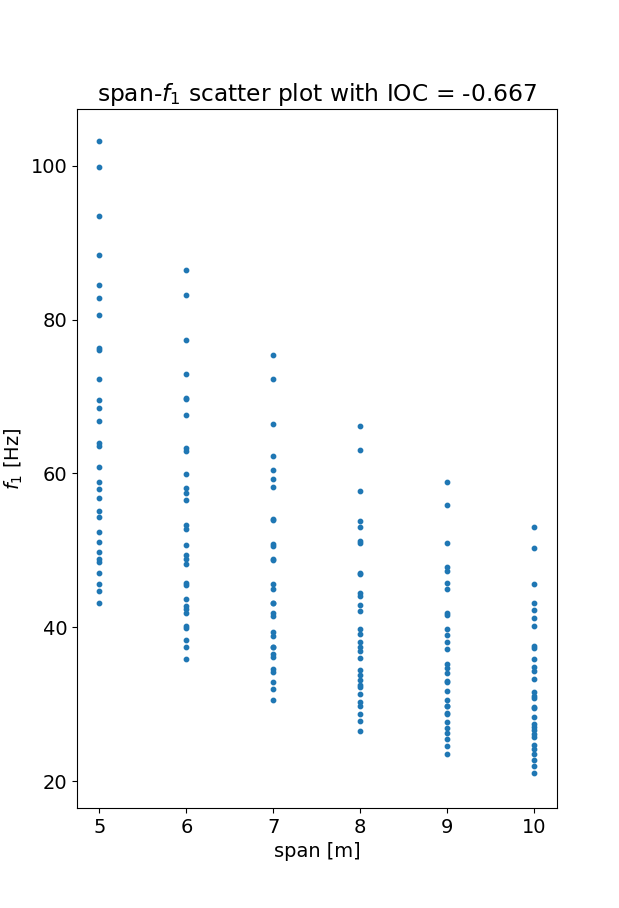
\includegraphics[width=.99\linewidth]{l_f1}
  \caption{$l-f_1$}
\end{subfigure}
~
\begin{subfigure}[b]{.32\textwidth}
  \centering
  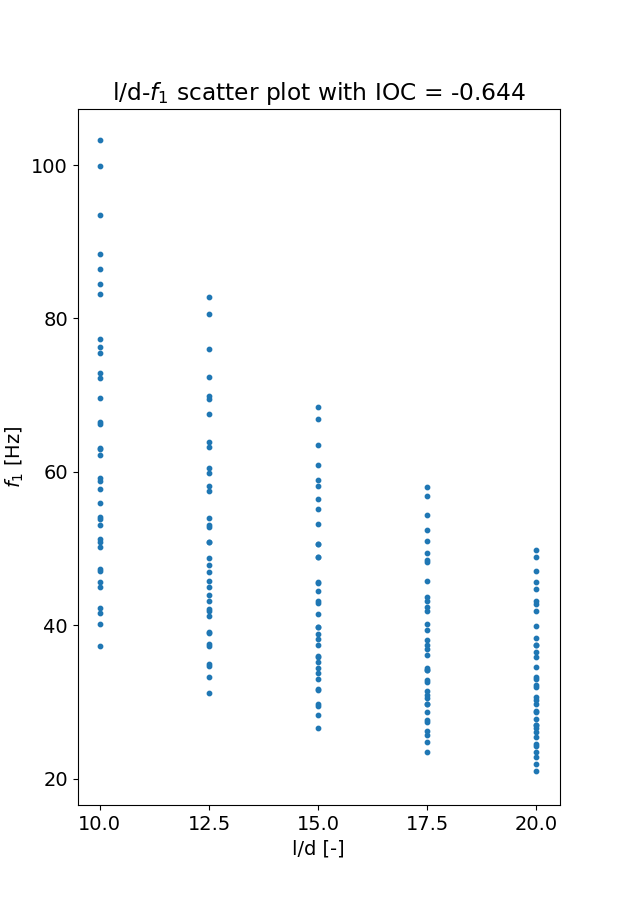
\includegraphics[width=.99\linewidth]{l2d_f1}
  \caption{$l/d-f_1$}
\end{subfigure}
~
\begin{subfigure}[b]{.32\textwidth}
  \centering
  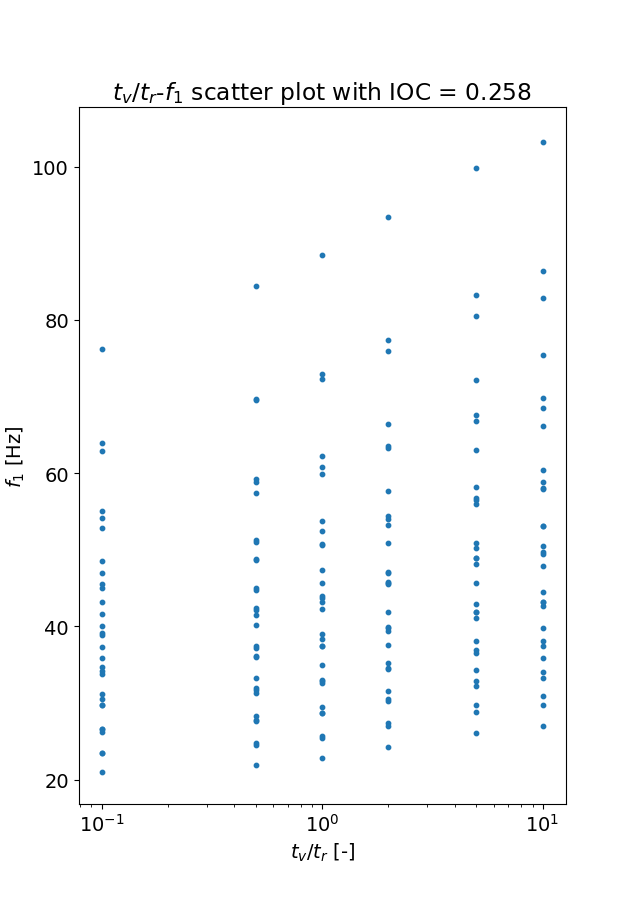
\includegraphics[width=.99\linewidth]{gamma_f1}
  \caption{$t_v/t_r-f_1$}
\end{subfigure}

\caption{Geometric parameters-natural frequency (first mode) scatter plot}
\label{fig:geom-f1}
\end{figure} 

It is interesting to observe that the natural frequency drops with increasing span. As span is the only index in the three geometric parameters that has a unit, a concrete number, instead of a dimensionless ratio that represents a scalable model. Plot (a) indicates that the natural frequency has a size effect, the bigger the size is, the lower natural frequency it shows. An increase in $l/d$ results in an reduction in frequency as the arch effect is weaker. The $t_v/t_r$ ratio does not influence the natural frequency much (with slightly positive effect), which can be explained by $\omega_n=\sqrt{k/m}$. For the vault, k and m are roughly evenly distributed everywhere, for the ribs, where there is less mass also shows less stiffness, so the ratio can keep more or less the same. 

Figure \ref{fig:m1_f1} shows the $m_1-f_1$ scatter plot, there exists no clear correlation between the two modal parameters.

\begin{figure}[H]
\centering
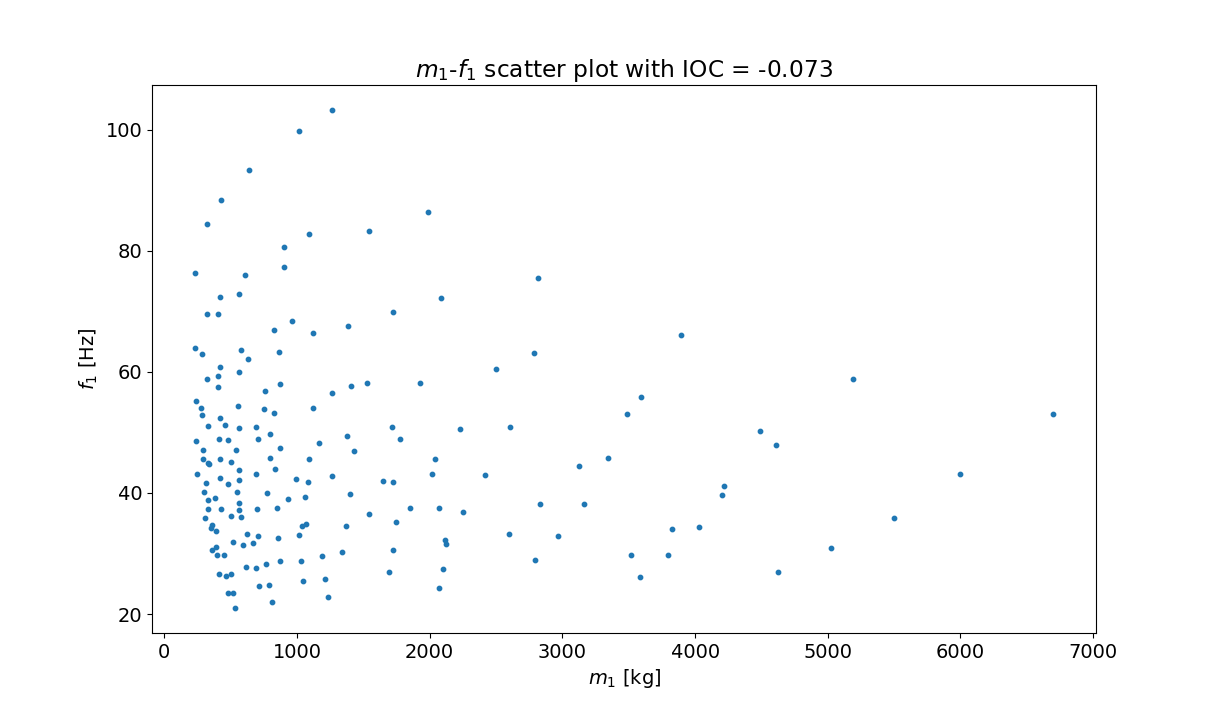
\includegraphics[width=1\textwidth]{images/m1_f1}
\caption{$m_1 - f_1$ scatter plot}
\label{fig:m1_f1}
\end{figure}


\subsection{Mode shape}
All floors show similar first 6 mode shapes as illustrated in figure \ref{fig:mode_shapes}. As stated above, the $t_v/t_r$ ratio influences the area involved in vibration. The ribs tend to restrict the vibration in a smaller region in the middle and impose constraint on the vault near edges. It also can be described from another side, the vault tens to disperse the vibration to a larger region, figure \ref{fig:first_modes} is the demonstration. When the vault dominates, the region with large vibration amplitude expands compared to a ribs dominating floor.
\begin{figure}[H]
\centering
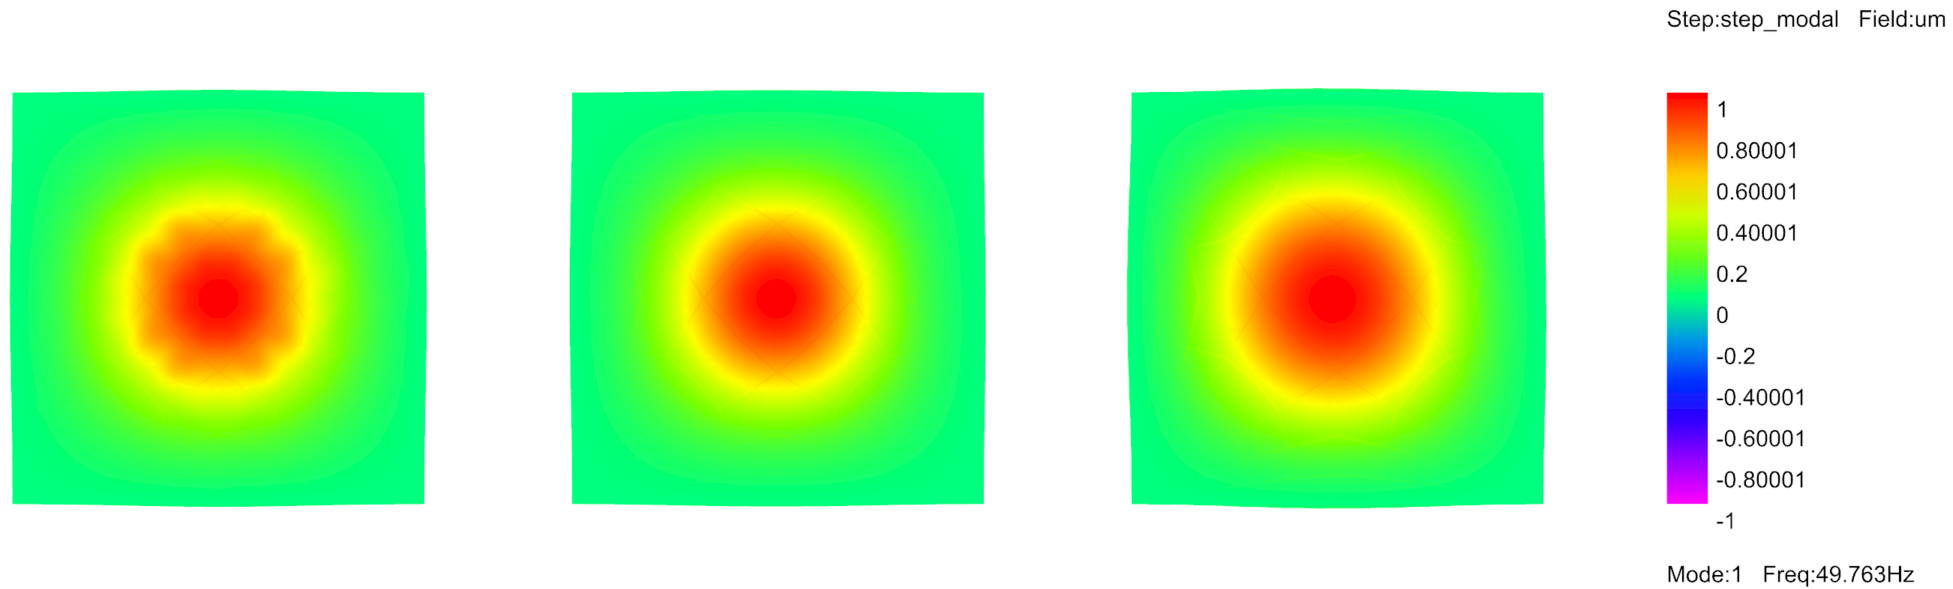
\includegraphics[width=1\textwidth]{images/first_modes}
\caption{first mode shapes with $t_v/t_r=0.1,1,10$ from left to right}
\label{fig:first_modes}
\end{figure}

\section{Solution of response time history}
The theoretical background and solving procedure have been described in section \ref{subsec:modal_superposition} and \ref{subsec:resp_time_histroy}. The equation of motion in modal coordinate and the response time history via modal superposition were solved based on equation \ref{eqn:motion_q} and \ref{eqn:u} in Python. It is very necessary to compare the results from Python with those from Abaqus for calibration.
\subsection{Modeling in Abaqus}
An Abaqus model of a floor with $l=5m, l/d=20, t_v/t_r=1$ was built. This model is imported from the Rhino mesh model, so the models for Abaqus and for Python are exactly the same, except for the definition of damping. In Python, the damping ratio $\xi=3\%$ is defined for all modes, as it is a feature of a mode. In Abaqus, however, the definition of damping is executed in material module. For the Rayleigh damping, the damping matrix consists of the mass-proportional damping and the stiffness-proportional damping,
\begin{equation}
    \mathbf{c}=\alpha\mathbf{m}+\beta\mathbf{k}
\end{equation}
\noindent
where $\alpha$ represents the mass coefficient and $\beta$ the stiffness coefficient. The damping ratio related to each mode varies along with the angular frequency (as shown in figure \ref{fig:damping}):
\begin{equation}
    \xi_n=\frac{\alpha}{2\omega_n}+\frac{\beta\omega_n}{2}
\end{equation}
\noindent
To solve $\alpha$ and $\beta$, damping ratios from two modes $i, j$ are needed. The damping ratio of modes in between will be underestimated, while outside of the range overestimated. The damping ratio of the first mode should be precisely set to be 3\%. If the other mode is the 2nd mode, damping ratios of all later modes will be overestimated. The choice of the mode $j$ is model dependent, it hinges on the complexity (number of DOFs) of the model and number of modes that effectively participate in vibration. Considering that this mesh model has 13211 elements and the first 25 modes may be effectively involved in vibration, the damping ratio of the 10th mode is set to be $3\%$. Then the calculated $\alpha$ and $\beta$ were given in Abaqus, and a calculation with standard (implicit) solver for dynamics was launched.
\begin{figure}[H]
\centering
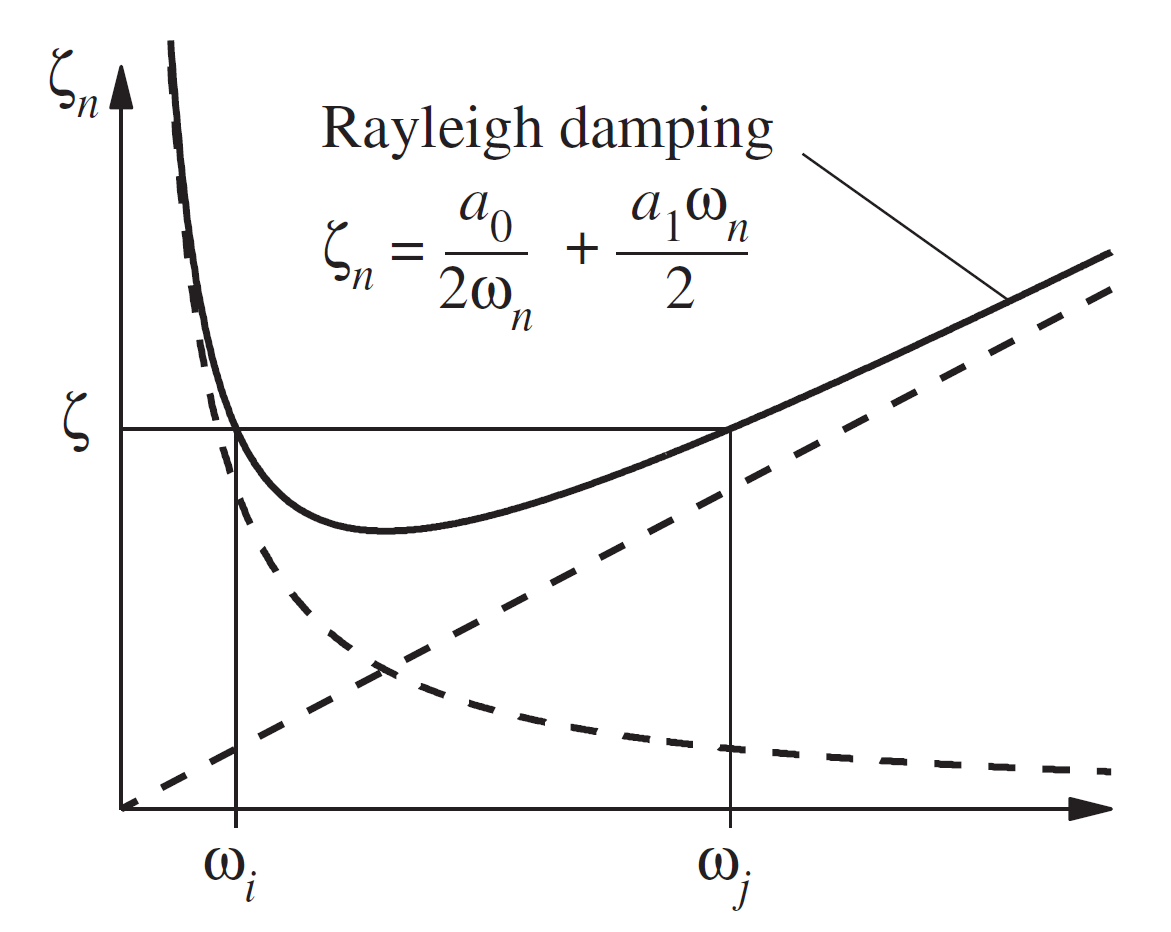
\includegraphics[width=0.5\textwidth]{images/damping}
\caption{Damping ratio in relation to angular frequency \cite{chopra2007dynamics} with notation $a_0=\alpha$, $a_1=\beta$ }
\label{fig:damping}
\end{figure}
\subsection{Calibration of results with Abaqus}
The results of response time history analysis from Abaqus and Python are compared in figure \ref{fig:response_abq}. 100 modes are used for modal superposition, and the contribution of the first mode is also plotted. It shows a very good match of the data. The results from modal superposition present a slightly lower value in displacement, which is reasonable as not all modes have involved. Then they show a slightly higher value in acceleration and rms-acceleration, suggesting a conservative evaluation. Such response indicates a very typical transient phase, where the structure vibrates at its natural frequencies right after the excitation and the energy dissipates quickly through damping. Afterwards, the structure will calm down and step into the steady phase, where the vibration continues but at the excitation frequency. The peak of rms-acceleration always appears at the first moment when it is calculated, namely at 0.5s, in all studied floors.

\begin{figure}[H]
\centering
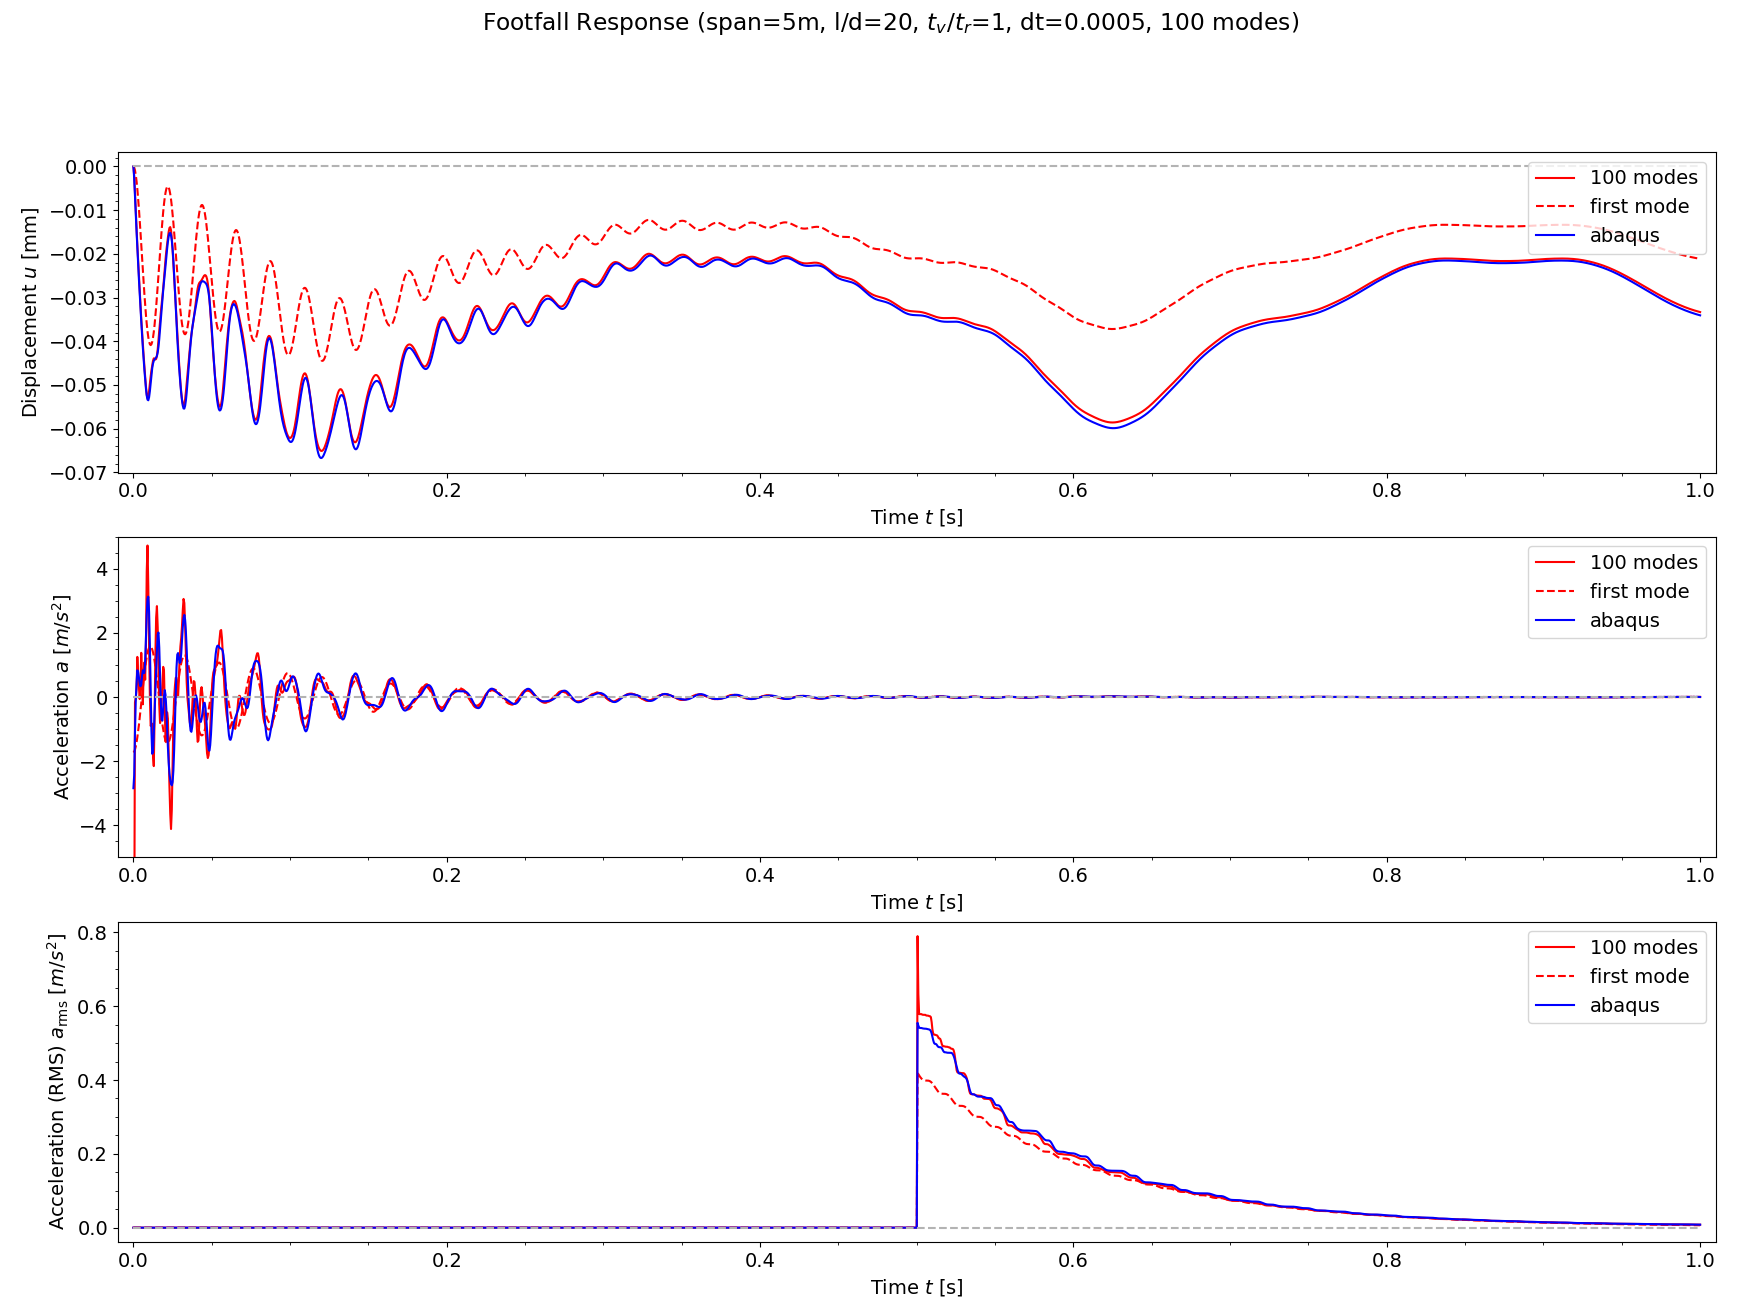
\includegraphics[width=1\textwidth]{images/response_abq.png}
\caption{Comparison of footfall response calculated by Abaqus and by Python with modal superposition}
\label{fig:response_abq}
\end{figure}

This plot also indicates that the first mode is not enough to represent the displacement or acceleration. In addition, there appears a peak in rms-acceleration that derives from an unrealistically high acceleration that is no shown in the acceleration subplot. The complete picture of the subplot is shown in figure \ref{fig:acc_whole}. This unrealistic value takes place at the first calculation time interval, and it stems from the derivation of velocities in high modes. These problems will be fixed to a large degree when the frequency weighting takes part in the evaluation. 
\begin{figure}[H]
\centering
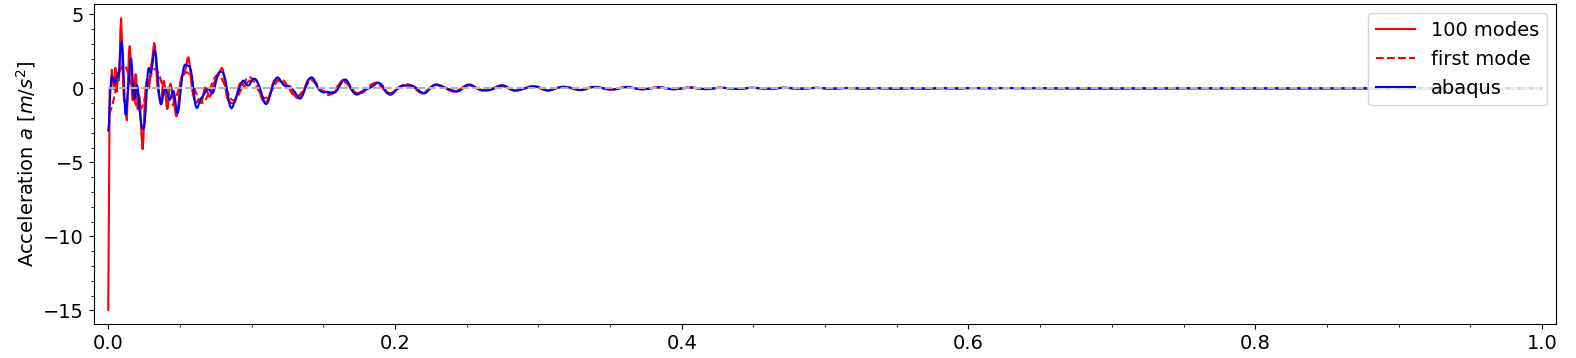
\includegraphics[width=1\textwidth]{images/acc_whole}
\caption{The whole picture of acceleration with extreme value}
\label{fig:acc_whole}
\end{figure}

\subsection{Frequency weighted response}
Note that for the rms-acceleration subplot in figure \ref{fig:response_abq}, the frequency weighting is not introduced.Figure \ref{fig:acc_weight} shows both the original and weighted rms-acceleration. It is clear that the frequency weighting plays a very important role by reducing the response by 70\% for this floor. It also can be seen that the response from the first mode can represent the total response quite well, more than 88\% of the total response is contributed by the first mode. Moreover, the frequency weighting has a peak clipping effect by filtering out the response from high modes.

\begin{figure}[H]
\centering
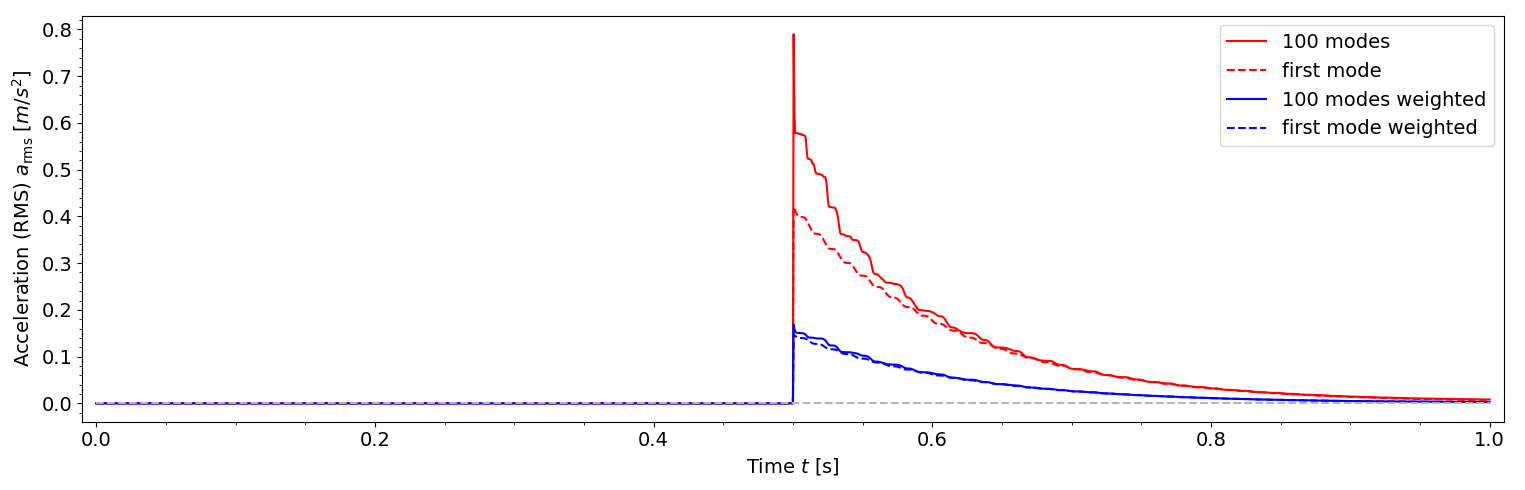
\includegraphics[width=1\textwidth]{images/acc_weight}
\caption{Original and weighted rms-acceleration}
\label{fig:acc_weight}
\end{figure}

\subsection{Number of modes for modal superposition}
One important issue in solution of the response is the proper number of modes for superposition. On the one hand, it can not be too few so that the response loses its accuracy. On the other hand, it should not be too high so that the computation becomes unaffordable or uneconomic. The recognition of important modes then become significant. Some modes are more effectively activated than others, they tend to (but not necessarily) contribute more in the total response. 

Figure \ref{fig:res_part_factor} shows the unweighted and weighted response factor as well as participation factor in relation to modes involved in modal superposition. Again, the figure illustrates the significance of frequency weighting. The unweighted response factor continues increasing even when 100 modes are adopted, whereas the weighted response factor shows a plateau after 30 modes. The modal participation factor is a modal parameter that indicates whether a mode is effectively activated or not. It is formulated in equation \ref{eqn:Gamma} and repeated here for convenience:
\begin{equation}
    \label{eqn:Gamma_1}
    \Gamma_n=\frac{\boldsymbol{\phi}_n^T\mathbf{s}}{M_n}
\end{equation}
\noindent
It is further used for the calculation of modal load
\begin{equation}
    P_n(t)=\Gamma_nP(t)
\end{equation}
\noindent
Only when the mode shape $\boldsymbol{\phi}$ and spatial distribution vector \textbf{s} are in alignment with each other, a large participation factor, namely a considerable load will be applied on this mode. Where there is a high participation factor, there appears an increase in response factor, although to different degrees. Several modes that are effectively activated (mode 1,6,11,15) and not activated (mode 23) are listed for visualization and comparison. For mode 11, because the largest displacement is not in the middle, so the middle point is not normalized as 1 but a negative value, resulting in a negative participation factor with less magnitude.

\begin{figure}[H]
\centering
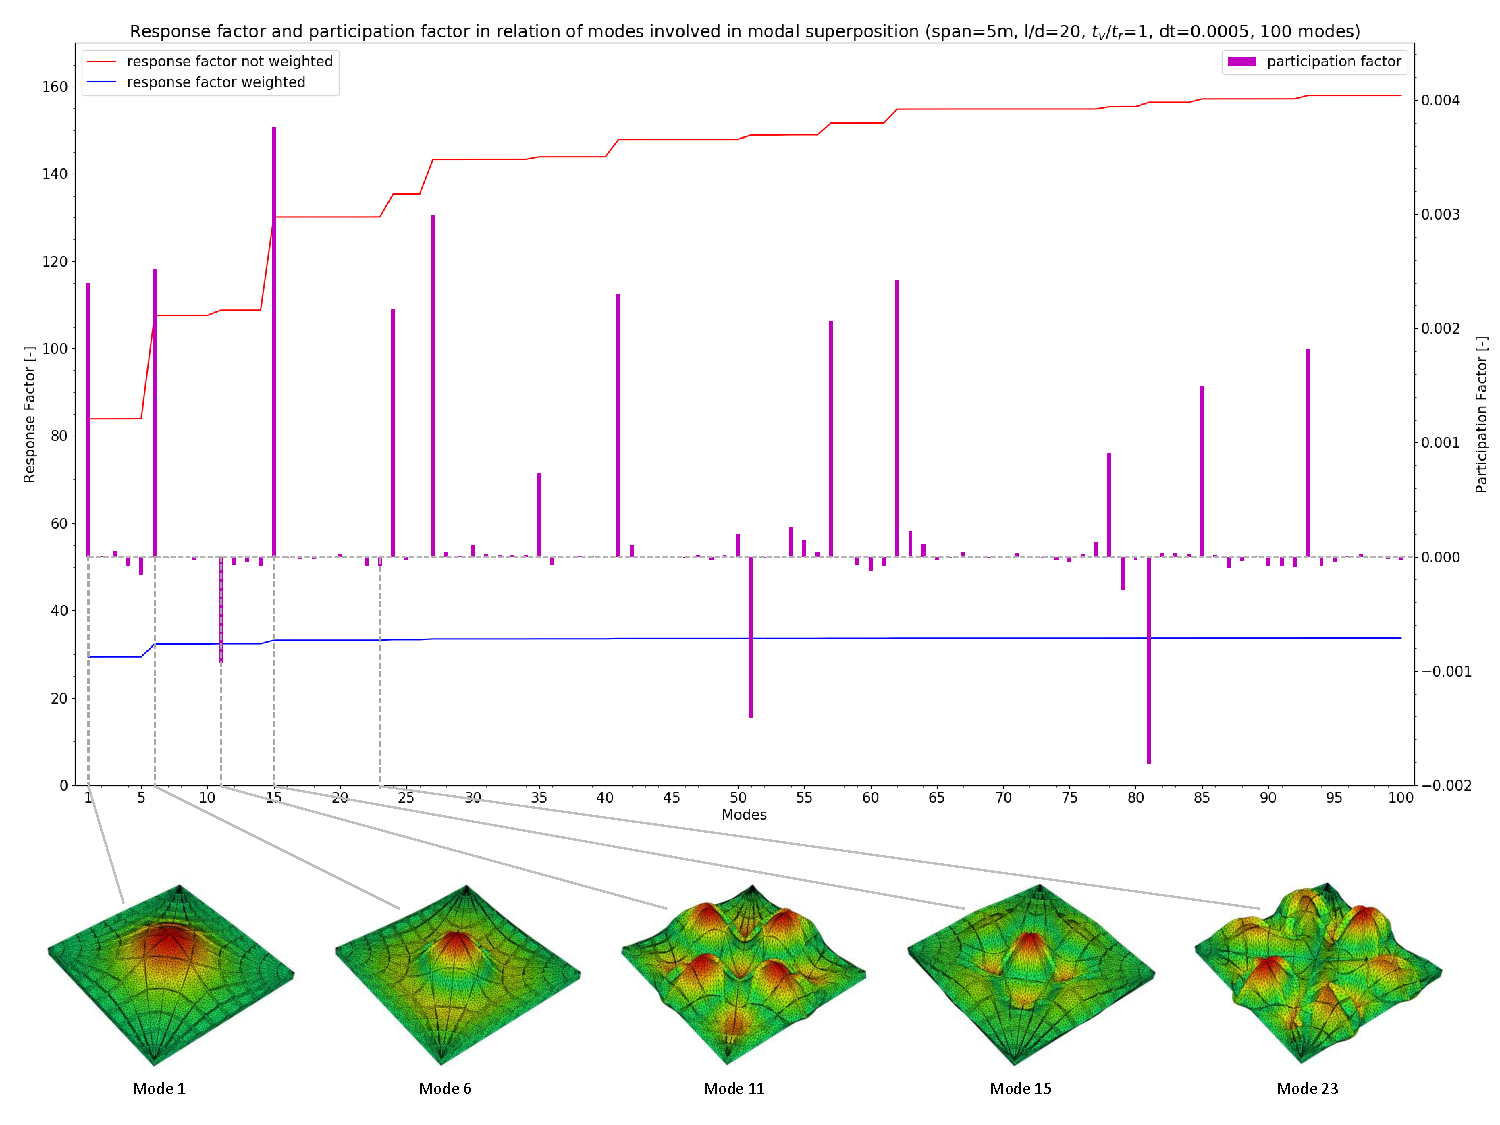
\includegraphics[width=1\textwidth]{images/res_part_factor.pdf}
\caption{Response factor and participation factor in relation to modes involved in modal superposition}
\label{fig:res_part_factor}
\end{figure}

It is worth mentioning that the modal participation factor does not imply the actual contribution of the mode to the total response. Because to solve the equation of motion in modal coordinates
\begin{equation}
\ddot{q_n}+2\xi_n\omega_n\dot{q_n}+\omega_n^2q_n=\Gamma_nP(t)
\label{eqn:motion_q_1}
\end{equation}
\noindent   
damping ratio $\xi_n$ and angular frequency $\omega_n$ also play a role. Given that the damping ratio holds the same for all modes, a higher angular frequency will result in a lower solution of the modal coordinate. That's the reason why even with similar participation factors, higher modes tend to contribute less than lower modes. An objective indicator of the actual contribution would be modal contribution factor, which is defined as the ratio of response associated with certain mode to the total response
\begin{equation}
    \Bar{r}_n=\frac{r_n}{r}
\end{equation}
\noindent
The contribution factor shown in figure \ref{fig:contr_factor} indicates that the unweighted response has more contribution from modes other than the first mode, while the weighted response heavily relies in the first mode. Generally, the contribution of the first mode to the weighted response varies from 86\% to 92\% for all studied floor models, therefore the response from the first mode is a good indicator of the total response.  
\begin{figure}[H]
\centering
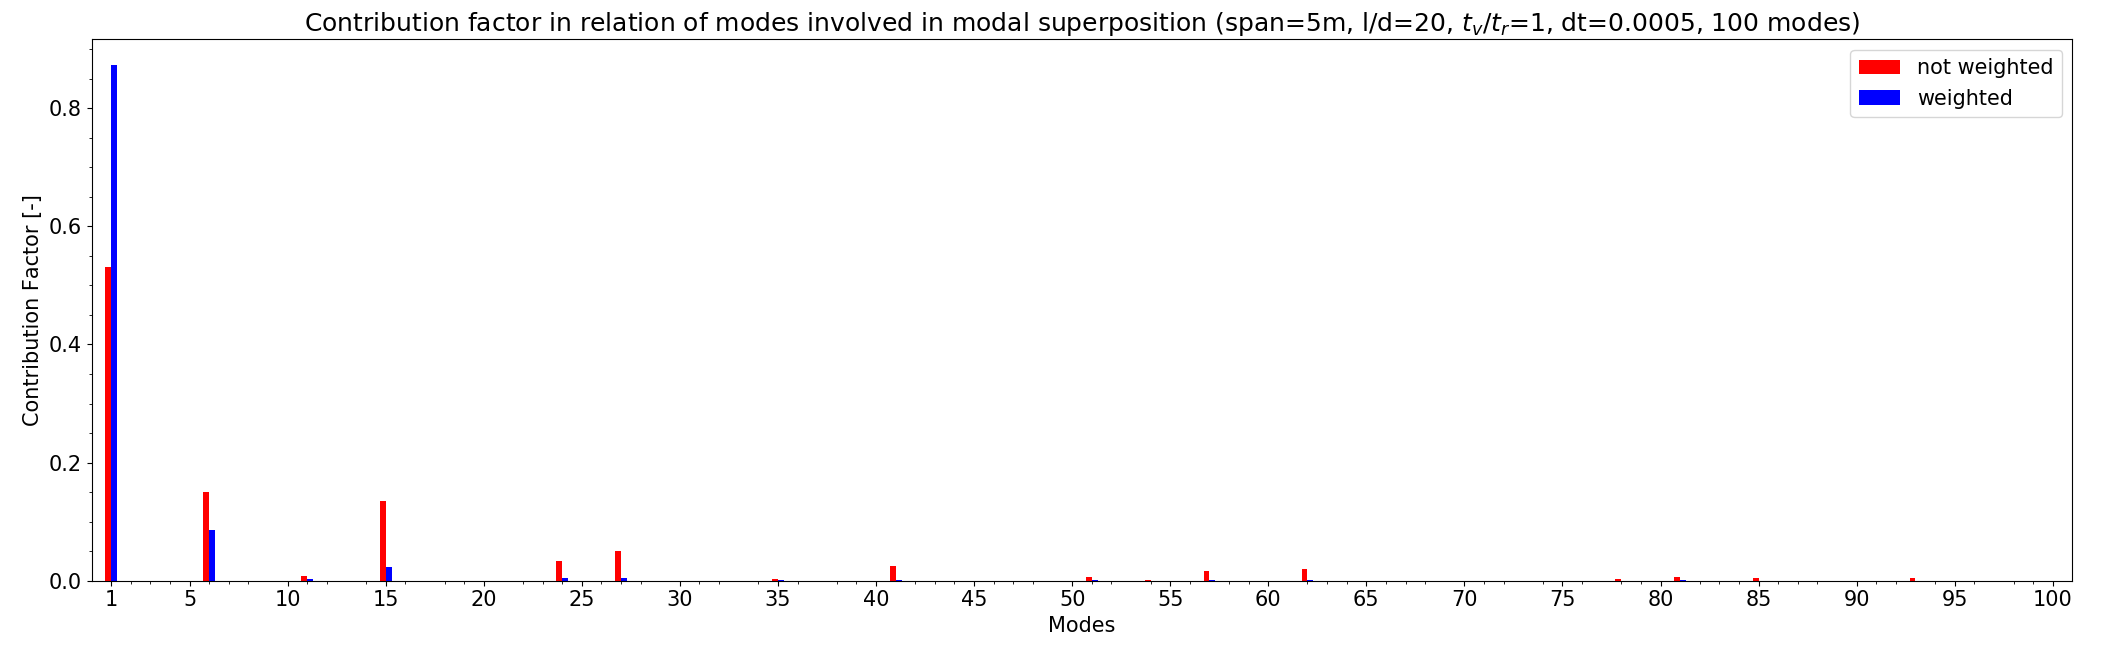
\includegraphics[width=1\textwidth]{images/contr_factor}
\caption{Contribution factor in relation to modes involved in modal superposition}
\label{fig:contr_factor}
\end{figure}

Although the weighted response factor keeps almost unchanged after 30 modes for the floor with $l=5m, l/d=20, t_v/t_r=1$, 50 modes are used for the calculation of all floors. The reason is that this floor has a fundamental frequency of $f_1=76$ Hz, which leads to a very strong frequency weighting effect. There are also some other floors with fundamental frequencies as low as 20 Hz that need more modes for superposition, because responses from high modes cannot be effectively filtered out and they will make considerable contribution to the total response.

\subsection{Advantages of modal superposition}
The implementation of response time history analysis via modal superposition in Python, instead of directly using existing FEM software like Abaqus, has the following advantages:
\begin{itemize}
    \item Much faster than Abaqus standard solver for dynamics. For the floor shown above, the smallest one among all floors, Abaqus took almost 2 hours, while the modal analysis in Abaqus and modal superposition in Python together took around 6 min for 100 modes, 4 min for 50 modes.
    \item Possibility of access to each mode, which is crucial for the post-process of the original response, for example frequency weighting. Abaqus has also modal superposition based dynamic solver, which took almost the same time as Python. It does not, however, provide the possibility to access to each mode, or only possible in a cumbersome way. 
    \item More structural insight into the its dynamic behavior. The solution of the response time history is no longer a black box, but a transparent one in which the correlation among parameters can be explained and checked.
\end{itemize}


\section{Evaluation of dynamic performance}
\subsection{Influence of geometric parameters}
The dynamic performance of the 180 floors with all different $l,l/d,t_v/t_r$ combinations were evaluated. The dynamic performance is characterized by the weighted response factor (called response factor later in the text and R in plots for simplicity). 
Figure \ref{fig:geom-R_contour} shows the influence of the geometric parameters on the response factor. In each subfigure the $l/d,t_v/t_r-R$ contour lines of a certain span are plotted. Take span=5m for example, the contour lines are smooth, the contour of response factor ranges from 4.0 to 56.0. The response increases in the positive direction of $l/d$ axis and negative direction of $t_v/t_r$ axis, which means a shallow and ribs dominating floor will have a large dynamic response. This observation matches with previous conclusion associated with modal mass and natural frequency in section \ref{subsec:modal_mass} and \ref{subsec:natural frequency}. The $l/d$ ratio does not influence modal mass much, but a high $l/d$ implies a low natural frequency, which results in a less pronounced frequency weighting effect and consequently a higher response factor. The $t_v/t_r$ ratio, on the contrary, shows an obvious positive correlation with the modal mass but almost no influence on the natural frequency. A lower $t_v/t_r$ value indicates a lower modal mass, which means that it is easier to get mobilized by a certain excitation based on the Newton's second law $a=F/m$. 

When the responses of different spans are compared, two trends can be observed: a wider range of response factor (especially the upper bound) and a less important role of $l/d$ with increasing span. The former can be explained by the dropping natural frequency along with larger span and the increase in modal mass cannot compensate it when the $t_v/t_r$ ratio is very low. The latter may lie in the concentration of ribs on the sides in large spans. The increase in natural frequency with a lower $l/d$ value is credited to a more fully developed arch effect. Since more mass is concentrated in ribs around the edges, the arch effect is weakened, so the $l/d$ value cannot influence the natural frequency much. More generally speaking, the natural frequency will not increase if the mass and stiffness distribution is not adequately optimized according to $\omega_n=\sqrt{k/m}$.

\begin{figure}
\begin{subfigure}[b]{.49\textwidth}
  \centering
  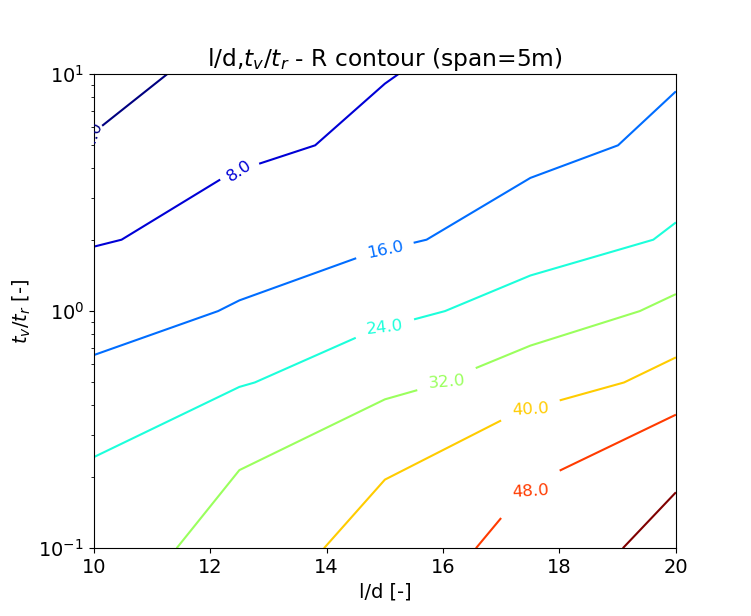
\includegraphics[width=.99\linewidth]{images/l2d,gamma_R_5m.png}
  \caption{span=5m}
\end{subfigure}
~
\begin{subfigure}[b]{.49\textwidth}
  \centering
  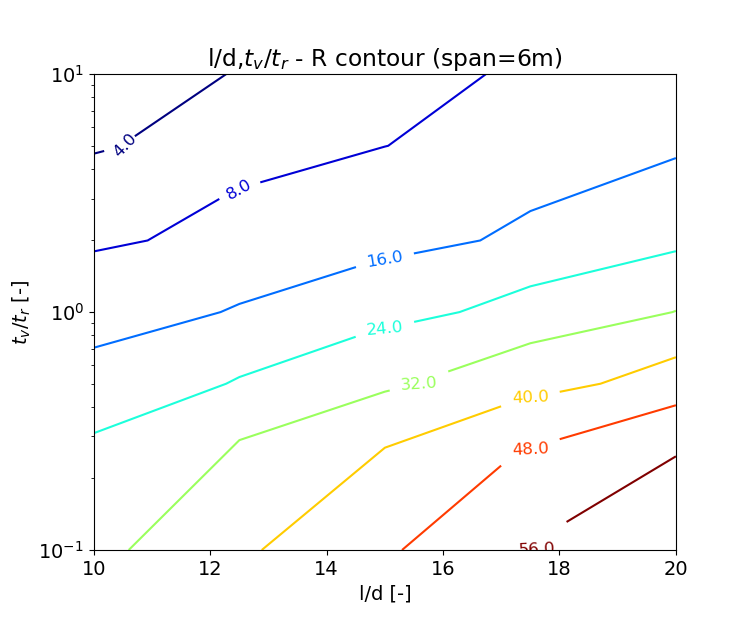
\includegraphics[width=.99\linewidth]{images/l2d,gamma_R_6m.png}
  \caption{span=6m}
\end{subfigure}

\begin{subfigure}[b]{.49\textwidth}
  \centering
  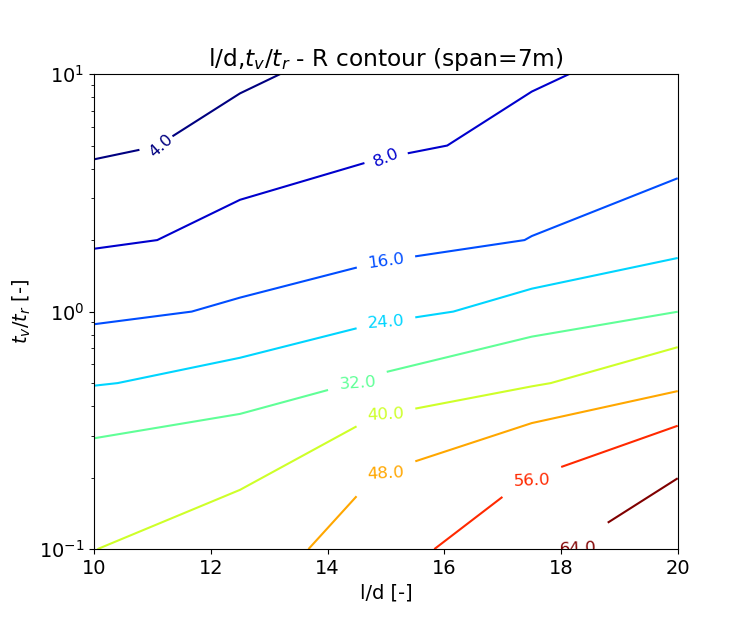
\includegraphics[width=.99\linewidth]{images/l2d,gamma_R_7m.png}
  \caption{span=7m}
\end{subfigure}
~
\begin{subfigure}[b]{.49\textwidth}
  \centering
  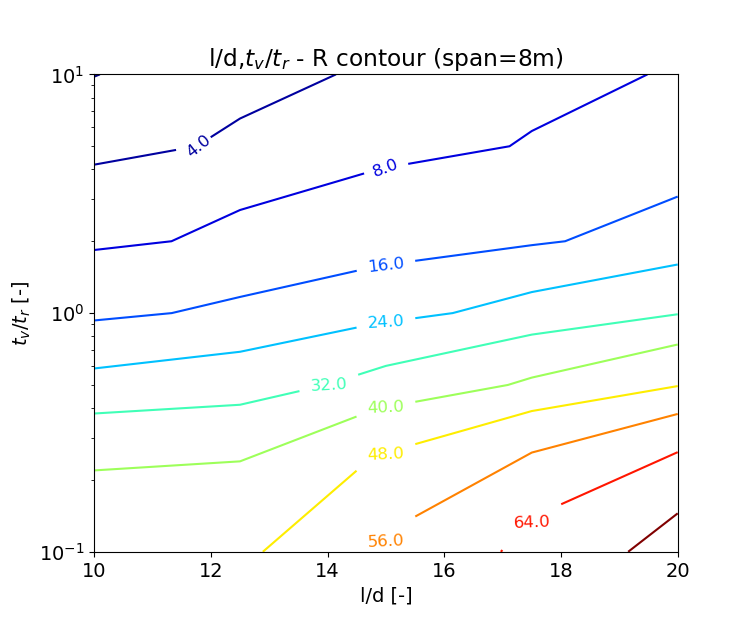
\includegraphics[width=.99\linewidth]{images/l2d,gamma_R_8m.png}
  \caption{span=8m}
\end{subfigure}

\begin{subfigure}[b]{.49\textwidth}
  \centering
  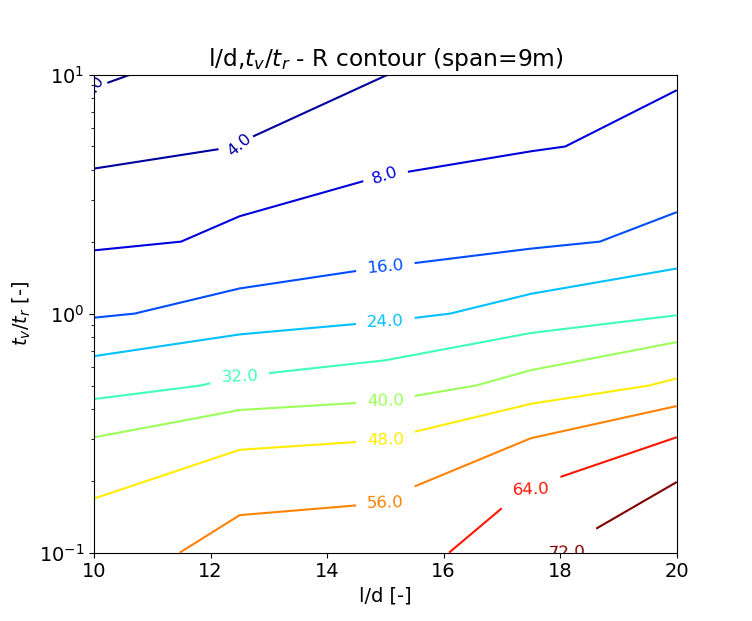
\includegraphics[width=.99\linewidth]{images/l2d,gamma_R_9m.png}
  \caption{span=9m}
\end{subfigure}
~
\begin{subfigure}[b]{.49\textwidth}
  \centering
  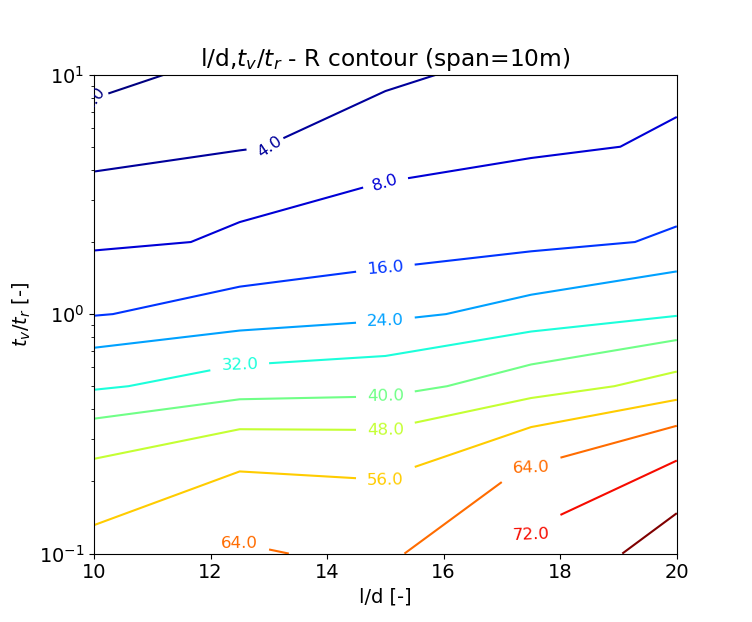
\includegraphics[width=.99\linewidth]{images/l2d,gamma_R_10m.png}
  \caption{span=10m}
\end{subfigure}

\caption{Geometric parameters-response factor contour plot}
\label{fig:geom-R_contour}
\end{figure} 

The relation between the geometric parameters and the response factor can also be depicted with input/output correlation scatter plot as shown in figure \ref{fig:geom-R_scatter}. It indicates that the span has very little influence on the dynamic performance, $l/d$ ratio has some importance and the $t_v/t_r$ has the greatest significance. This importance sequence conforms well to the decision-making power of engineers. Floors with different spans, which are usually not determined by engineers, can behave equally well or badly. $l/d$ ratio, in which engineers may participate in the decision, can have some influence on the dynamic behaviour. Through $t_v/t_r$ ratio, which can be decided by engineers to a large extent, the dynamic performance can be greatly altered (optimized if in a good way). Of course, such coincidence is valid only under the given pattern and scaling scheme.

\begin{figure}[H]
\begin{subfigure}[b]{.32\textwidth}
  \centering
  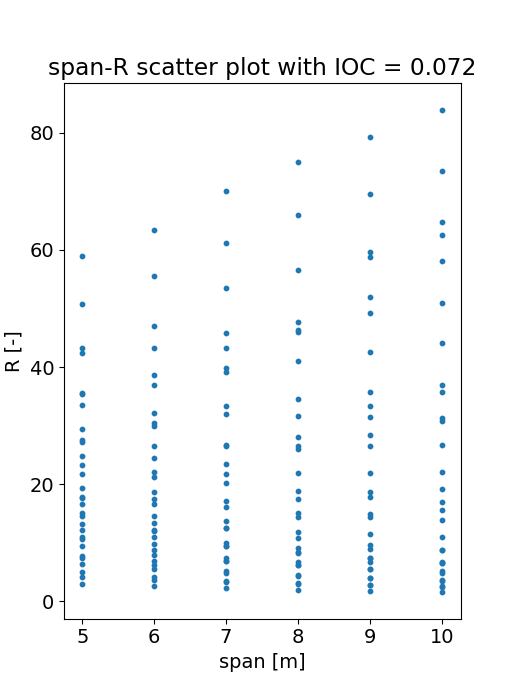
\includegraphics[width=.99\linewidth]{span_R}
  \caption{$l-R$}
\end{subfigure}
~
\begin{subfigure}[b]{.32\textwidth}
  \centering
  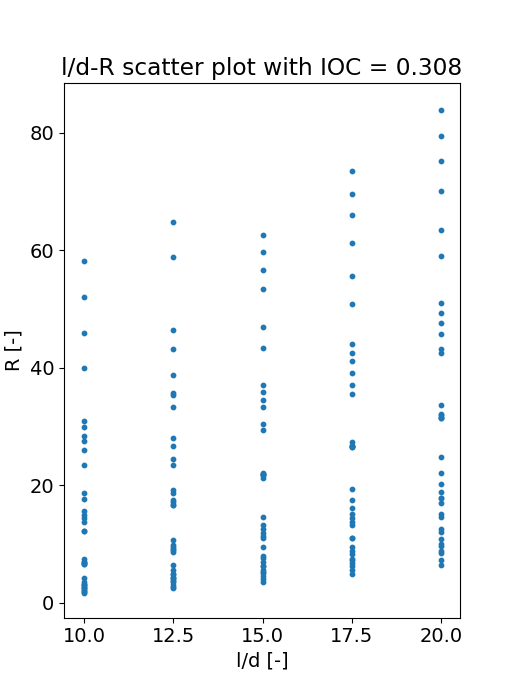
\includegraphics[width=.99\linewidth]{l2d_R}
  \caption{$l/d-R$}
\end{subfigure}
~
\begin{subfigure}[b]{.32\textwidth}
  \centering
  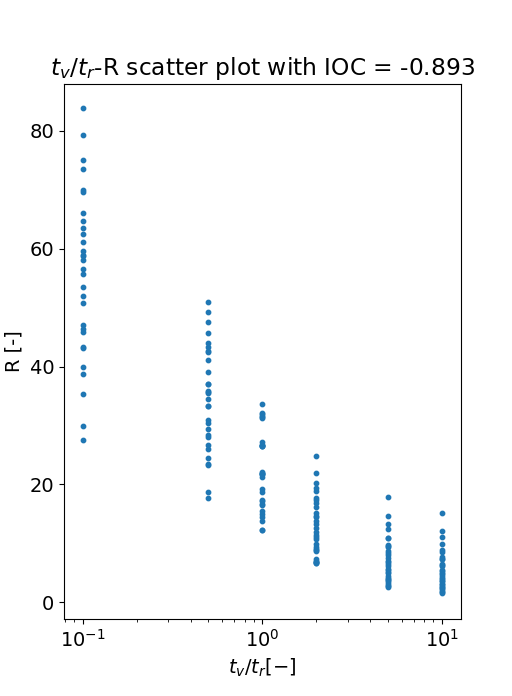
\includegraphics[width=.99\linewidth]{gamma_R}
  \caption{$t_v/t_r-R$}
\end{subfigure}

\caption{Geometric parameters-response factor scatter plot}
\label{fig:geom-R_scatter}
\end{figure}


\subsection{Influence of modal parameters}
\label{subsec:influence of modal parameters}
The influence of geometric parameters on the response factor is actually not direct. Whatever the change in geometry, it will firstly reflected in the modal properties, and then the dynamic performance. The relation between geometry and modal properties has been explored in section \ref{sec:modal analysis}. The next step would be to analyze how the modal parameters influences the dynamic behavior. As the modal parameters are always related to a certain mode, a clear relation only exists in the modal properties and the modal response resulted from them. Since the first mode makes the overwhelmingly dominant contribution to total response, the findings related to the first mode can be applied to the overall behaviour to a great extent.

Modal mass, natural frequency and mode shape are the three modal parameters that take part in the calculation and influence the response factor. Figure \ref{fig:m1,f1_R1_contour} shows the $m_1,f_1-R_1$ contour of different spans. "Coincidentally", the contour lines from different spans are in alignment with each other. This is actually no coincidence, no matter how different the geometry of two floors is, as long as they have the same modal properties, they are identical in modal space and have the same response. The small deviations among different spans may lie in the interpolation when making the contours and the similar but not identical mode shapes. 

It can be found that a higher natural frequency and a greater modal mass will both contribute to a lower response factor, but to a different degree depending on the initial situation. The gradient of the contour lines implies that the frequency has a greater impact when the modal mass is already high, or when the frequency is still low. The modal mass plays a greater role when the floor already shows a high frequency or a low modal mass. This finding indicates that if a floor has a very low modal mass or a very high natural frequency, the most efficient way to improve the dynamic performance is to increase the modal mass, instead of trying to further raise its natural frequency, and vice versa. This may further imply that, for a floor with a short span, which is usually accompanied with a low modal mass, improvements should be taken to increase the modal mass. A thinkable way is to add mass where  necessary and efficient. Whereas for a large span floor, which is likely to already have a high modal mass, measures to increase the natural frequency will be preferred. Probably removing material from where redundant is better than adding mass. The high frequency of the vaulted floor is just achieved by removing redundant material. 

\begin{figure}[H]
\centering
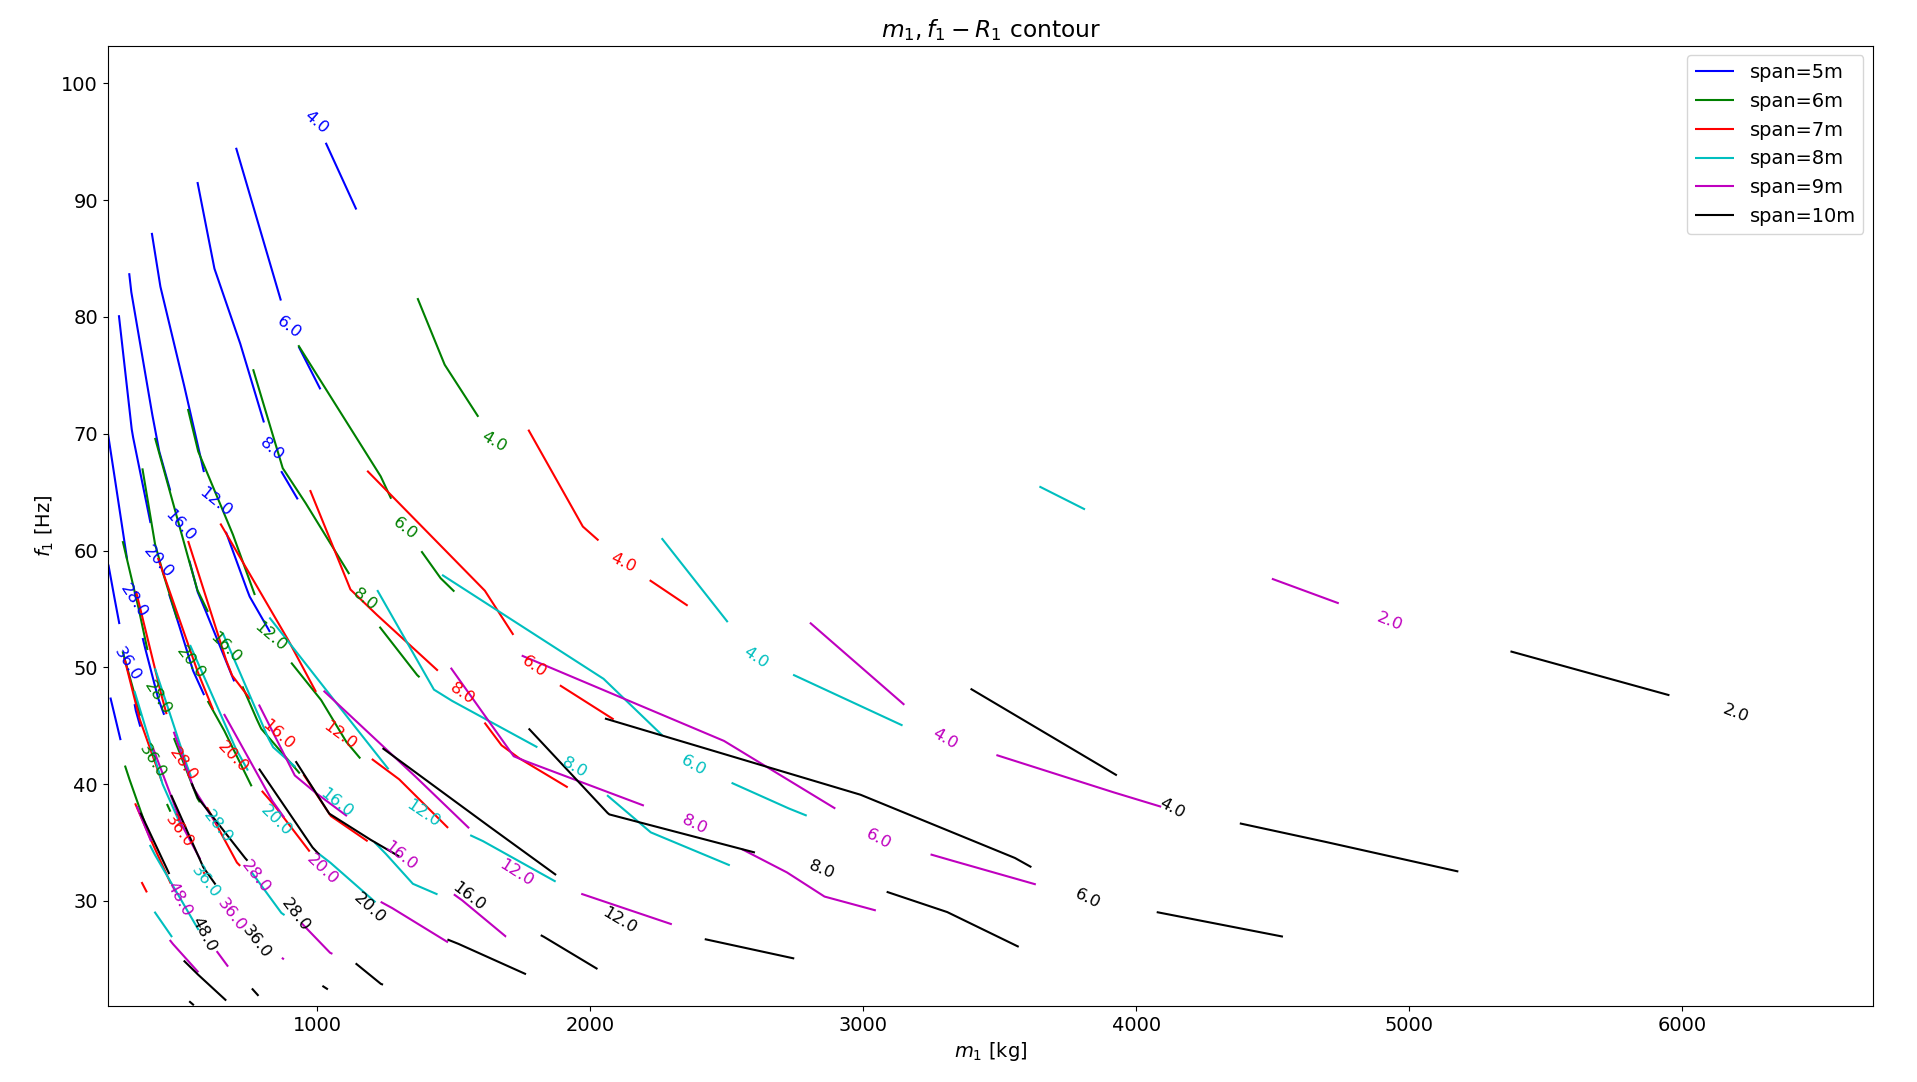
\includegraphics[width=1\textwidth]{images/m1,f1_R1}
\caption{$m_1,f_1-R_1$ contour plot}
\label{fig:m1,f1_R1_contour}
\end{figure}

As stated above, figure \ref{fig:m1,f1_R1_contour} is independent from the concrete geometry, this property may endow it a new utility - "table look-up". As long as $m_1$ and $f_1$ are known, the response factor can be directly read off or interpolated from this plot. The solution of response time history and post-processing of the data can be skipped, thus a quite amount of time can be saved. This can be practical for a quick check of the response after the modal analysis, it can also serve as the "objective function" to minimize for an optimization process. Compared with solely $m_1$ or $f_1$ as the objective function, $R_1$ is a more proper quantity that is directly associated with the actual performance. 

Figure \ref{fig:m1,f1_R1_contour} and figure \ref{fig:geom-R_contour} both describe the dynamic characteristics of the series of floors, but in a different way. The former is more for academic use, as the modal analysis has to be carried out as the first step. The independence from the concrete geometry makes it universal, it does not, however, provide any clue how to change $m_1$ and $f_1$ in an expected direction in the real world. Figure \ref{fig:geom-R_contour} is a rather engineer plot, which tells the engineer how to change the geometric parameters to achieve an acceptable performance, but it limits itself to a very specific geometry.

The influence of $m_1$ and $f_1$ on $R_1$ can also be depicted by input/output correlation plot, as shown in figure \ref{fig:m1,f1_R1_scatter}. The influence of the modal mass is enormous, very high responses are only possible when the modal masses are very low. The impact of the natural frequency is also considerable, the response factor tends to decrease when the natural frequency raises.

\begin{figure}[H]
\begin{subfigure}[b]{.49\textwidth}
  \centering
  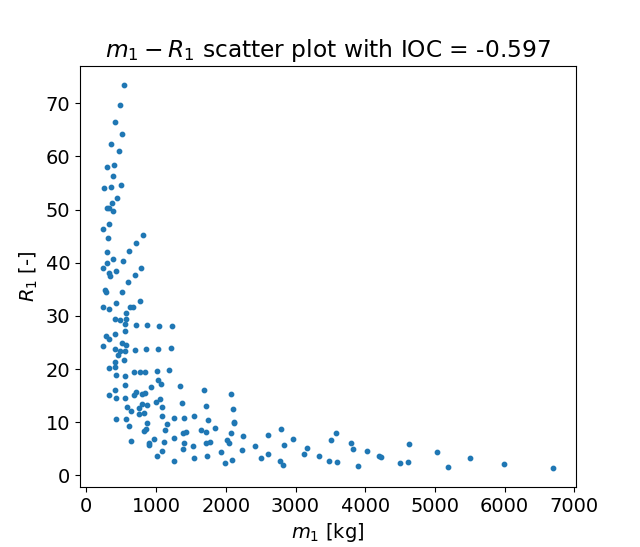
\includegraphics[width=.99\linewidth]{m1_R1}
  \caption{$m_1-R_1$}
\end{subfigure}
~
\begin{subfigure}[b]{.49\textwidth}
  \centering
  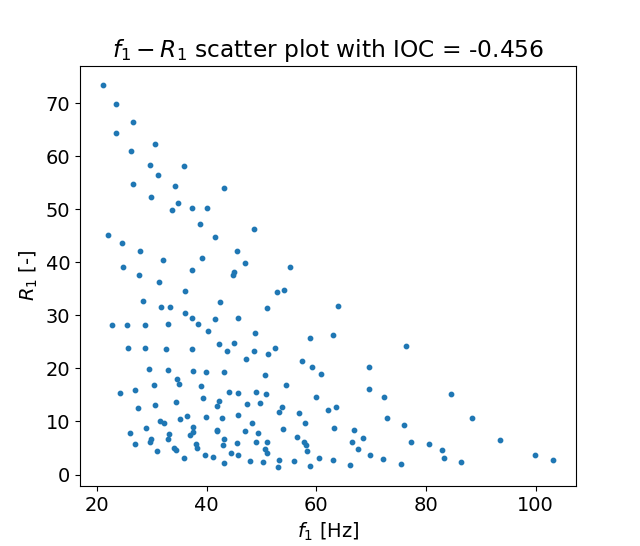
\includegraphics[width=.99\linewidth]{f1_R1}
  \caption{$f_1-R_1$}
\end{subfigure}

\caption{Modal parameter- modal response factor scatter plot}
\label{fig:m1,f1_R1_scatter}
\end{figure}

From the previous analysis, it can be concluded that $t_v/t_r, m_1, f_1$ are the three most important parameters that influence the response factor $R_1$. These parameters are not independent, it will be meaningful to see their correlation in one plot. Figure \ref{fig:norm_m1_f1_R1} illustrates the normalized $m_1,f_1,R_1$ (normalized by $t_v/t_r=0.1$) in relation to $t_v/t_r$. It shows a very interesting "mirrored" relation between normalized modal mass and normalized response factor while the normalized frequency keeps almost constant around 1. The "mirrored" relation in log scale indicates an inverse proportional relationship in normal scale, which is exactly the relation suggested by SCI P354 expressed in equation \ref{eqn:SCI} and by the calculation of participation factor $\Gamma_n$ expressed in equation \ref{eqn:Gamma}. This mirror is even rigorous in sequence in terms of specific $l$ and $l/d$. The mirror, however, is not very rigorous in values, for example, the normalized $m_1,f_1,R_1$ written in tuple ($m_{1,n},f_{1,n},R_{1,n}$)=(20.23,1.42,0.029) for $l=5m, l/d=10, t_v/t_r=10$, the product of $m_{1,n}\times R_{1,n}=20.23\times 0.029=0.59$ is not even close to 1, that lies in the normalized frequency that deviates already considerably from 1 (the influence of frequency will be discussed later). This plot also shows the great improvements that can be achieved by changing the $t_v/t_r$ ratio, the response could drop to 3\%-25\% of the response with $t_v/t_r=0.1$. Such great improvements are directly related to the huge increase in modal mass.
\begin{figure}[H]
\centering
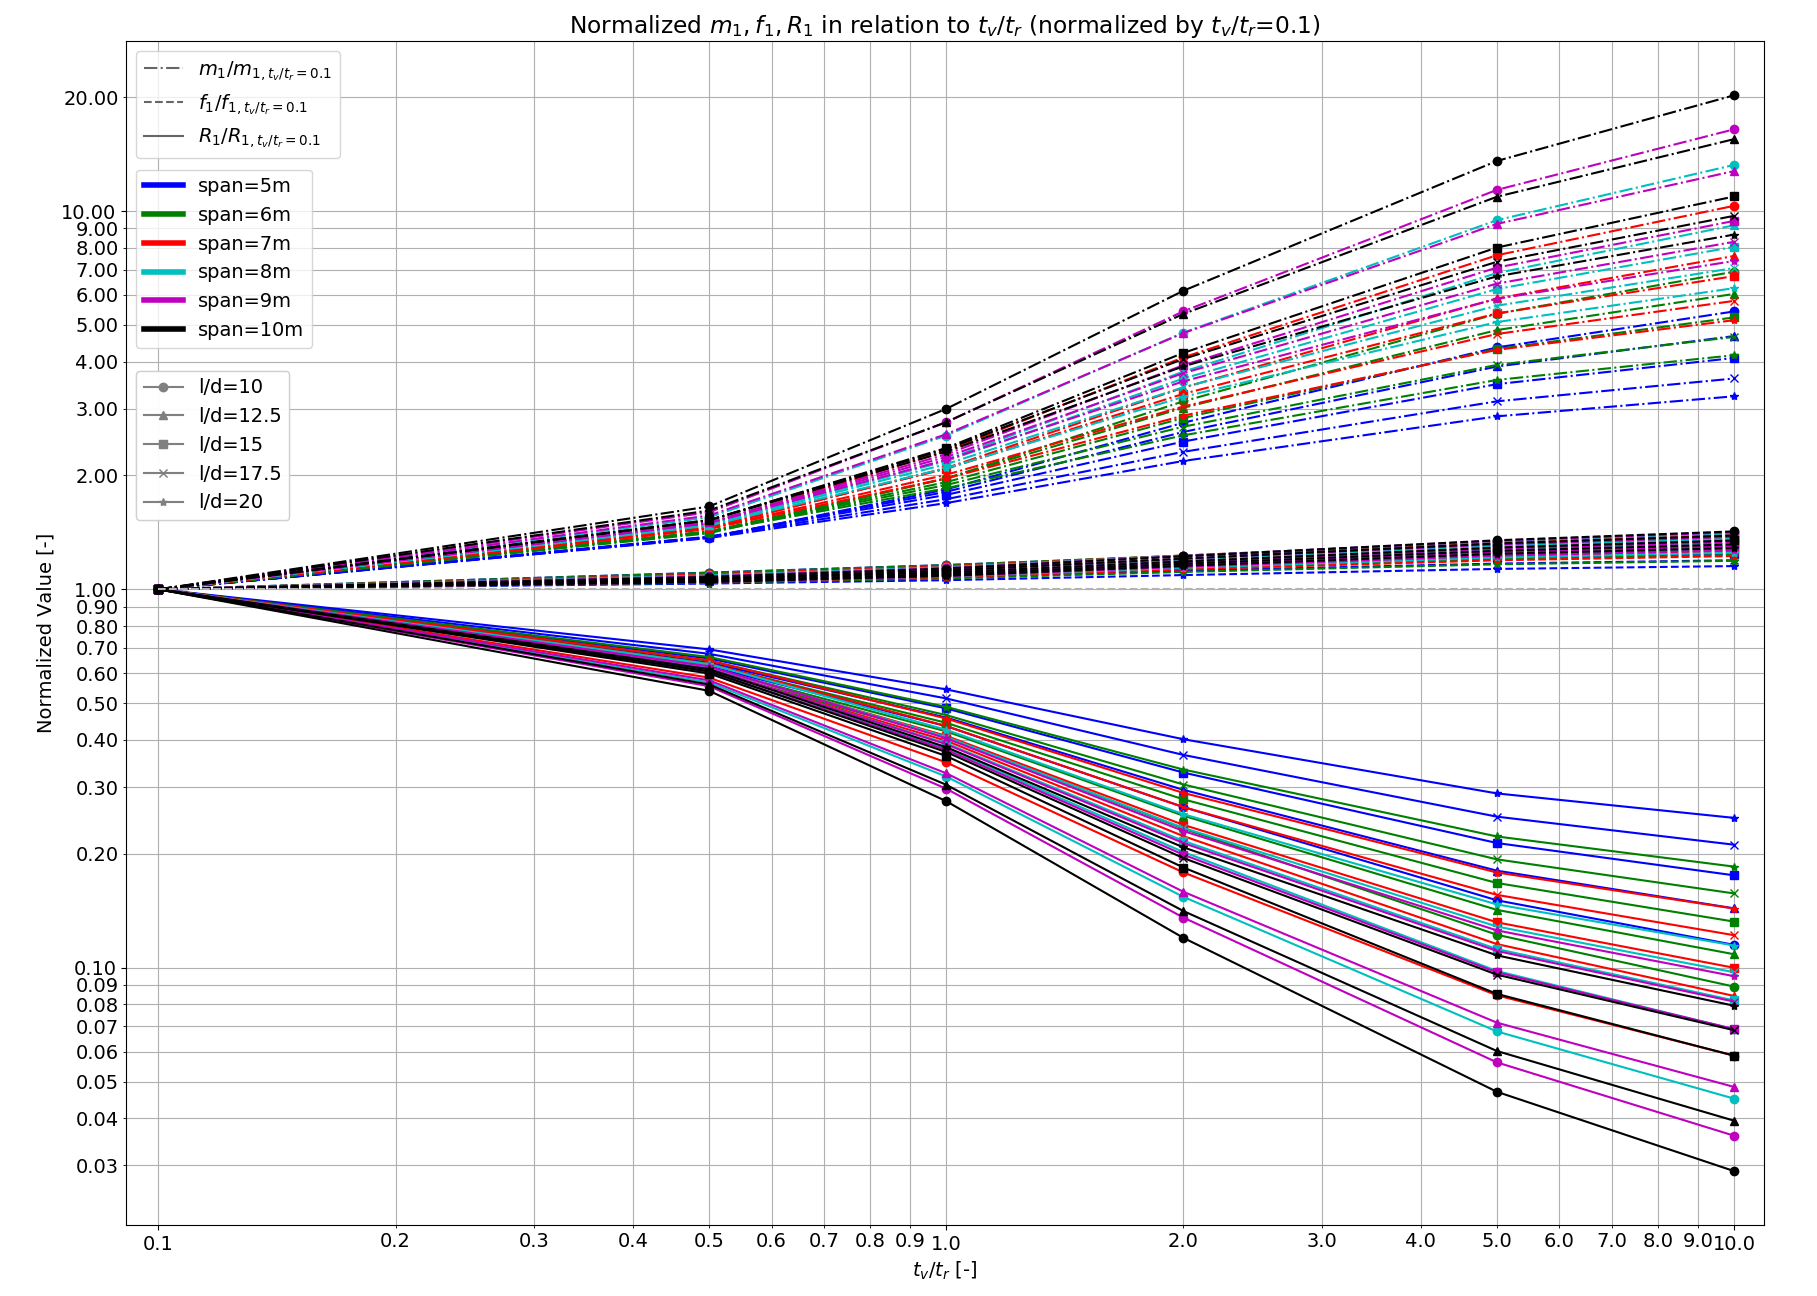
\includegraphics[width=1\textwidth]{images/norm_m1_f1_R1}
\caption{Normalized $m_1,f_1,R_1$ in relation to $t_v/t_r$}
\label{fig:norm_m1_f1_R1}
\end{figure}

The mathematical relation between natural frequency and response factor is less direct. To ward off the influence of the modal mass, ($m_1,f_1,R_1$) tuples with constant $m_1$ should be selected. One can see from figure \ref{fig:m1,f1_R1_scatter} that there are relative concentrated points around $m_1=850$ kg. 18 points with $m_1=[1\pm10\%]\times850$ kg are chosen, and normalized by point 0 with ($m_1,f_1,R_1$)=(813.0,22.0,45.1). Figure \ref{fig:norm_m1_f1_R1_const_m1} shows the results. It depicts a roughly mirrored figure, but the normalized $f_1$ values seem to be not high enough in position. When the exponent of $f_1$ is raised to 1.5, the figure turns out to present a well shaped mirrored figure, as shown in figure \ref{fig:norm_m1_f1_1_5_R1_const_m1}. It means that the response factor is in inverse proportion to $f_1^{1.5}$ when the $m_1$ keeps constant. The over inverse proportional relation is not without reason. Firstly, the natural frequency influences the response factor through the frequency weighting function (see figure \ref{fig:Wb}) $W_b=16/f_1$ when $f_1>16$ Hz, which applies to all floors. Secondly, the natural frequency also intervenes in the solution of response time history expressed in equation \ref{eqn:motion_q}, a raise in $\omega_n$ will lead to a drop in $q_n(t)$, and thus in response. 
\begin{figure}[H]
\centering
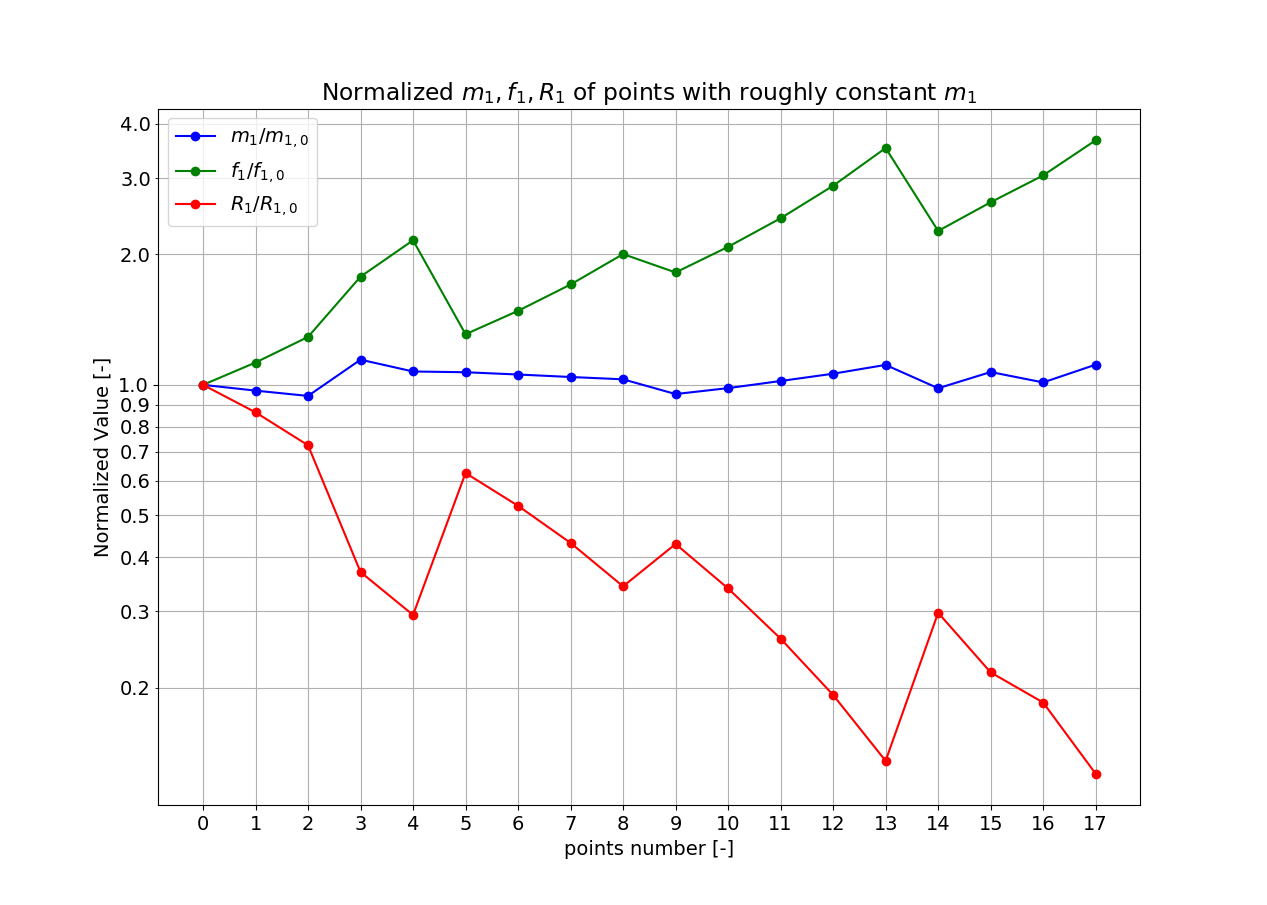
\includegraphics[width=.8\textwidth]{images/norm_m1_f1_R1_const_m1.png}
\caption{Normalized $m_1,f_1,R_1$ of points with roughly constant $m_1$}
\label{fig:norm_m1_f1_R1_const_m1}
\end{figure}

\begin{figure}[H]
\centering
\includegraphics[width=.8\textwidth]{images/norm_m1_f1_1_5_R1_const_m1.png}
\caption{Normalized $m_1,f_1^{1.5},R_1$ of points with roughly constant $m_1$}
\label{fig:norm_m1_f1_1_5_R1_const_m1}
\end{figure}

Combining the effect of modal mass and natural frequency, the response factor can be expressed as:
\begin{equation}
    R_1\sim \frac{1}{m_1f_1^{1.5}}
\label{eqn:R1}
\end{equation}
When the tuple ($m_{1,n},f_{1,n},R_{1,n}$)=(20.23,1.42,0.029) is used to calibrate this formula:
\begin{equation}
    \frac{1}{m_{1,n}f_{1,n}^{1.5}}=\frac{1}{20.23\times1.42^{1.5}}=0.029\approx R_{1,n}
\label{eqn:R1_n}
\end{equation}
they match very well.

Note that equation \ref{eqn:R1} only represents a proportional relation, not a concrete formula, it applies to \ref{eqn:R1_n} as there normalized values are used. The equivalent expression would be:
\begin{equation}
    R_1= \frac{C}{m_1f_1^{1.5}}
\label{eqn:R1(m1_f1)}
\end{equation}
where $C$ is a constant that can be obtained by calculating the mean of all data points. After evaluation, the constant $C=3778622$. 

Figure \ref{fig:m1,f1_R1_pred} shows the true and predicted data points in modal space. The precision of prediction is measured by the MSE (mean square error) index
\begin{equation}
    MSE=\frac{1}{n}\sum_{i=1}^n(\hat{y}_i-y_i)^2
\end{equation}
\noindent
The true and predicted data points are almost superposed, the $MSE$ is as low as 0.264\%. Equation \ref{eqn:R1(m1_f1)} unveils the quantitative relation between modal response factor and modal parameters, which may make further response time history analysis redundant. It needs to be pointed out that this equation is only valid for floors with natural frequency $f_1>16$ Hz, otherwise the frequency weighting function $W_b$ will have other forms, so will this equation. That is probably is reason why this formula differs from equation \ref{eqn:SCI} greatly in the exponent of $f_1$.

\begin{figure}[H]
\begin{subfigure}[b]{.49\textwidth}
  \centering
  \includegraphics[width=.99\linewidth]{m1_R1_pred}
  \caption{$m_1-R_{1,\text{true}},R_{1,\text{pred}}$}
\end{subfigure}
~
\begin{subfigure}[b]{.49\textwidth}
  \centering
  \includegraphics[width=.99\linewidth]{f1_R1_pred}
  \caption{$f_1-R_{1,\text{true}},R_{1,\text{pred}}$}
\end{subfigure}

\caption{True and predicted modal response factor in modal space}
\label{fig:m1,f1_R1_pred}
\end{figure}

The natural frequency seems to have less impact than the modal mass according to figure \ref{fig:m1,f1_R1_scatter}. This misconception stems from the narrower value range of natural frequency. The natural frequency ranges from 20 Hz to 100 Hz (5 times), while modal mass from 230 kg to 6700 kg (29 times), so the effect of modal mass seems much more dramatic. Nonetheless, these ranges may also indicate the relative difficulty in changing the two parameters.
\chapter{Optimization of the floor for dynamic performance}
\label{chap5}
Among the studied 180 floors, only 49 of them (27.2\%) have reached the acceptance criterion that the response factor $R$ should not exceed 8 for office buildings under single person excitation, as shown in figure \ref{fig:m1_f1_fail}. The border differentiating acceptable floors and failed floors is easy to recognize, it is exactly the contour line $R=8$ in figure \ref{fig:m1,f1_R1_contour}. Since 72.7\%  of the floor have failed, improvement measures should be conceived. From the viewpoint of practical applications, however, this failure quotient does not have much meaning. It only means that under the artificial $l,l/d,t_v/t_r$ combinations and given scaling scheme, some of these slabs do not function well enough and the others do. If another scaling scheme is given, e.g. 30\% mass of a solid rectangular floor with the same outer geometry instead of 40\%, some acceptable floors right now will fail as well. So this chapter will not specifically deal with the failed floors, but more generally, how to improve dynamic performances of the rib stiffened vaulted floor.
\begin{figure}[H]
\centering
\includegraphics[width=.8\textwidth]{images/m1_f1_fail}
\caption{Acceptable/failed floors shown in $m_1-f_1$ scatter plot}
\label{fig:m1_f1_fail}
\end{figure}

\section{Improvements by mass addition}
Some direct improvement measurements are thinkable just according to the analysis so far. For example, a thicker floor (low $l/d$ value) will lead to a higher natural frequency, more uniformly distributed mass in vault (high $t_v/t_r$ value) can greatly raise the modal mass and slightly increase the natural frequency, the both changes can result in better performances. However, sometimes the $l/d$ ratio cannot be changed as much as it structurally needed, the $t_v/t_r$ ratio cannot go extreme due to production reasons, more refined improvements are necessary. 

The relation between modal response and modal parameters expressed in equation \ref{eqn:R1(m1_f1)} indicates that the raise of product $m_1f_1^{1.5}$ results in a better performance. For an adequately improved floor, for instance if the $t_v/t_r$ ratio has been already raised to a reasonable value, a simultaneous increase in modal mass and natural frequency becomes very difficult. The augment in one value is sometimes only possible at the cost of a reduction in the other. If this trade off can be controlled properly, there will exist space for further improvements. 

The increase in modal mass is easier to conceive and to realize than natural frequency, as the latter is associated with both the stiffness and mass of a structure. Figure \ref{fig:m1,f1_R1_contour} indicates that an increase in modal mass can effectively reduce the response when the modal mass is still low. This finding should apply to floors with 5m span.

The modal mass is computed by
\begin{equation}
\label{eqn:mn_1}
    m_n = \boldsymbol{\phi}_n^T\textbf{m}\boldsymbol{\phi}_n
\end{equation}
it is intuitive that if the mass distribution conforms to the mode shape, the matrix product will generate the highest value. Since the mode shape has its peak in the middle, the mass also should be more concentrated in the middle. One possible way is to keep the existing constant thickness in ribs and vault, and add more mass where appropriate. 

Four factors may influence the effectiveness of improvement: the region where mass is added, the way of adding mass, the amount of mass increase, the geometry of the floor. Two regions have been tried, one is the most inner area (middle 1), the other also includes the second inner ring of panels (middle 2), as shown in figure \ref{fig:middle_1_2}. It is assumed that the additional mass is uniformly distributed on the designated region. Two schemes of adding mass were introduced. One was to change the thickness, which changes the mass and stiff of the panels at the same time. The other scheme is to change the density, which means that only the mass will be altered and the stiffness keeps unchanged. The former simulates the additional mass as the structural component that is monolithically cast and later functions together with the main structure. The latter represents some filling material that solely adds the weight but without any stiffness contribution. The following mass increases in percentage of the original mass were set: [(5),10,(15),20,(25),30]\%. The percentage in brackets are additional mass increments for refinement of the calculation, if certain scheme of adding mass turns out to be better. Only floors of 5m span with following geometric parameters have been evaluated: l/d=[10,15,20], $t_v/t_r=[0.1,1,10]$.

\begin{figure}[H]
\begin{subfigure}[b]{.49\textwidth}
  \centering
  \includegraphics[width=.99\linewidth]{middle_1}
  \caption{Region middle 1}
\end{subfigure}
~
\begin{subfigure}[b]{.49\textwidth}
  \centering
  \includegraphics[width=.99\linewidth]{middle_2}
  \caption{Region middle 2}
\end{subfigure}

\caption{Two regions in the middle for additional mass}
\label{fig:middle_1_2}
\end{figure}

Figure \ref{fig:mass_inc_density_middle1} to figure \ref{fig:mass_inc_thickness_middle2} show the normalized (by initial floors) $m_1,f_1,R_1$ of optimized floors with different mass addition schemes and regions in relation to mass increases in percentage. It is evident that mass addition through density change (no stiffness increase) functions not well. The drop in natural frequency compensates much of the increase in modal mass, there appears even some increases in the response for certain combinations. The reduction in natural frequency can be well explained by $\omega_n=\sqrt{k/m}$, when k is unchanged and m increases. Mass addition by thickness change can greatly raise the modal mass, while keeping the drop in natural frequency to a limited degree. Consequently, the improvements are considerable. 
\begin{figure}[H]
\centering
\includegraphics[width=.99\textwidth]{images/mass_inc_density_middle1.png}
\caption{Normalized $m_1,f_1,R_1$ of optimized floor in relation to mass increase (span=5m, density change, middle 1)}
\label{fig:mass_inc_density_middle1}
\end{figure}

\begin{figure}[H]
\centering
\includegraphics[width=.99\textwidth]{images/mass_inc_density_middle2.png}
\caption{Normalized $m_1,f_1,R_1$ of optimized floor in relation to mass increase (span=5m, density change, middle 2)}
\label{fig:mass_inc_density_middle2}
\end{figure}

\begin{figure}[H]
\centering
\includegraphics[width=.99\textwidth]{images/mass_inc_thickness_middle1.png}
\caption{Normalized $m_1,f_1,R_1$ of optimized floor in relation to mass increase (span=5m, thickness change, middle 1)}
\label{fig:mass_inc_thickness_middle1}
\end{figure}

\begin{figure}[H]
\centering
\includegraphics[width=.99\textwidth]{images/mass_inc_thickness_middle2.png}
\caption{Normalized $m_1,f_1,R_1$ of optimized floor in relation to mass increase (span=5m, thickness change, middle 2)}
\label{fig:mass_inc_thickness_middle2}
\end{figure}

The convex shape of the normalized response factor curve indicates reducing performance improvements with raising mass increase percentage. 5\% and 10\% mass increases are most efficient in terms of improvement/mass increase ratio. Table \ref{tab:R1_improv} summaries the effect of mass addition by changing thickness and what that concretely means for the floor\textsuperscript{*} $l=5m, l/d=15, t_v/t_r=1$. The mass addition in region middle 1 seems to generate more response reduction than in middle 2. The defect is the thick vault that may intrude the free space underneath, because the existing vacant space above the vault is not enough for such mass increase. This can also be solved by increasing the height of ribs above the vault. Compared with 5\% mass increase in region middle 1, 10\% mass increase does not bring much improvement. The mass addition in region middle 2 needs less thickness increase to achieve the same mass raise. Although the 5\% mass increase cannot produce a response reduction as high as in middle 1, a higher mass increase can still bring further performance improvement to push the response nearer to the acceptance criterion. In this case, 5\% mass increase in middle 1 and 10\% mass increase in middle 2 are preferred, the final choice depends on other conditions (e.g. if the intrusion in space underneath allowable, if 10\% mass increase is acceptable) and potential further changes (e.g. raise the height of ribs in the middle to create more vacant space for additional structural mass).

{
\renewcommand{\arraystretch}{1.2}
\begin{table}[H]
\caption{Summary of response reduction by mass addition through thickness changing}
\label{tab:R1_improv}
\begin{tabular}{cccccc}
\Xhline{2\arrayrulewidth}
\textbf{region}           & \textbf{mass inc.} & \textbf{resp. red.} & \textbf{\begin{tabular}[c]{@{}c@{}}resp. red.\\ floor\textsuperscript{*}\end{tabular}}   & \textbf{\begin{tabular}[c]{@{}c@{}}thick. inc.\\ floor\textsuperscript{*}\end{tabular}} & \textbf{\begin{tabular}[c]{@{}c@{}}total thick.\\ floor\textsuperscript{*}\end{tabular}} \\ \Xhline{2\arrayrulewidth}
\multirow{2}{*}[-0.8em]{middle 1} & 5\%                    & 36\%-62\%                & \begin{tabular}[c]{@{}c@{}}54\%\\ $R_1: 18.9\xrightarrow{}8.8$\end{tabular}  & 0.106 m                                                                     & 0.163 m                                                                  \\ \cline{2-6}
                          & 10\%                   & 49\%-75\%                & \begin{tabular}[c]{@{}c@{}}66\%\\ $R_1: 18.9\xrightarrow{}6.5$\end{tabular}  & 0.212 m                                                                     & 0.269 m                                                                  \\ \hline
\multirow{2}{*}[-0.8em]{middle 2} & 5\%                    & 20\%-40\%                & \begin{tabular}[c]{@{}c@{}}31\%\\ $R_1: 18.9\xrightarrow{}13.1$\end{tabular} & 0.026 m                                                                     & 0.083 m                                                                  \\ \cline{2-6}
                          & 10\%                   & 35\%-60\%                & \begin{tabular}[c]{@{}c@{}}49\%\\ $R_1: 18.9\xrightarrow{}9.7$\end{tabular}  & 0.052 m                                                                     & 0.109 m                                                                  \\ \Xhline{2\arrayrulewidth}
\end{tabular}
\end{table}
}

These improvements can be illustrated in the $m_1,f_1-R_1$ contour plot \ref{fig:m1_f1_improve}. None of the four schemes are along the most efficient direction - the gradient of $m_1,f_1-R_1$ surface, namely the normal direction of contour lines. Sometimes, designated changes in modal parameters are difficult to realize in reality, as they are tightly correlated.

\begin{figure}[H]
\centering
\includegraphics[width=.95\textwidth]{images/m1_f1_improve}
\caption{Four improvement schemes presented on $m_1,f_1-R_1$ contour plot}
\label{fig:m1_f1_improve}
\end{figure}

\section{Surrogate model based optimization}
The research so far, even the improvements by mass addition, is based on the models with uniform thickness in ribs and vault. It is intuitive that a "perfectly" improved floor under constant mass will not have constant thickness everywhere in vault, so will not in ribs. 

\subsection{One-quarter mesh model}
To optimize the floor in a further step, the dimension of the model has to be raised. The dimension of a model represents its complexity, and also the degree of refinement. When $l,l/d$ are kept constant, the previous model has only two dimensions, the thickness of the vault and ribs. To refine the floor, the panels were assigned to 41 groups, each group could have a different thickness. To reduce the computational cost, only one quarter of the slab was modeled, as shown in figure \ref{fig:panels_modelling} (each group is given a different color). There are two boundary surfaces, they are named by their normal directions. To capture the mode shapes that are symmetric about both x and y axis, including the 1st mode, the DOFs on boundary surface x should not move along x axis, and the rotation around y axis should be fixed. For boundary surface y, movement along y and rotation around x should be constrained. The movement and rotation in other directions are free. In addition, the stiffness and mass of the boundary surfaces should be halved, as they are shared by neighboring quarters. Because the main stiffness of the boundary surfaces is in vertical direction, the halving can be roughly achieved by halving the thickness, although it creates inaccuracy in horizontal stiffness. Natural frequencies and modal masses of the one quarter model match well with the symmetric modes of the full model.
\begin{figure}[H]
\centering
\includegraphics[width=.9\textwidth]{images/panels_modelling}
\caption{One-quarter model of the floor with $l=5m,l/d=15$}
\label{fig:panels_modelling}
\end{figure}

\subsection{Work flow}
For such a complex model with 41 dimensions, manual optimization is impossible. Because the final response cannot be expressed in a closed form of geometric parameters (the thicknesses of the 41 group of panels), no matter implicit or explicit, and the number of dimensions is large, traditional derivative based algorithm is not a good option. One possible solution is the genetic algorithm, which is robust even when there are multiple local optima, the objective function is not smooth and the number of parameters is large. However, even though the GA can accelerate the convergence by selecting "good seeds" and filtering out bad ones, it still requires a large amount of runs of the model. Assume that the model has a population of 100, and needs 200 generations to get converged (already optimistic assumption), then 20000 runs are needed. If one evaluation of such a model needs 1 min, then one optimization process will take two weeks, which is hardly affordable. One possible way to address the optimize problem is to use a surrogate model, which can reflect the essence of the real model to a certain degree but takes muss less time to run.

The concept of optimization through a surrogate model is shown in figure \ref{fig:opt_flowchart}. This is a machine learning alike idea, the accuracy of the final results cannot be guaranteed. They depends on the input sampling, the complexity of the model, the amount of real data and the form of surrogate model, etc. To "train" the surrogate model, certain evaluations of the full model, namely experimental designs, are necessary. Using the real (geometric input, response factor output) data sets, parameters in the surrogate model can be determined. The GA optimization will be no longer applied on the full model, but the surrogate model that skips the intermediate steps and directly maps the geometric input to the response factor output. Once the optimization is finished, the input of the optimized surrogate model will be used to recalculate the authentic response factor. Because the optimized input is sometimes not within the input samples that were used to train the surrogate model, the prediction from it can be biased. They values predicted by the surrogate model usually show the trend, but not necessarily the exact numbers. 

\begin{figure}[H]
\centering
\includegraphics[width=.7\textwidth]{images/opt_flowchart}
\caption{Flow chart of surrogate model based optimization}
\label{fig:opt_flowchart}
\end{figure}

\subsection{PCE surrogate model}
The are several ways to build the surrogate model, PCE (polynomial chaos expansion), Kriging model, neural nets, etc. Subject to the limitation of the author's knowledge and time frame for the master's thesis, only the PCE model has been implemented. It does not mean that it is the best option.

PCE is usually applied in a stochastic process to solve uncertainty propagation problems. It can depict the uncertainty in the output resulted from the uncertainty in the input accurately  enough based on a limited number of experimental designs. The problem that PCE addresses has similarities and also difference with the present problem of the floors. They both have a certain bandwidth in which the input can vary, and both have only limited number of evaluations of the full model. The difference is that, the distribution (uncertainty) of the output is not a concern in this optimization problem, therefore some modifications of the classical PCE can be made.

To approximate the real model $\mathcal{M}(\boldsymbol{X}$), a surrogate truncated PCE model can be built
\begin{equation}
    Y=\mathcal{M}(\boldsymbol{X})\approx \mathcal{M}^{PC}(\boldsymbol{X})=\sum_{\alpha\in \mathcal{A}}y_{\alpha}\Psi_{\alpha}(\boldsymbol{X})
\end{equation}
\noindent
The task is then to develop a set of appropriate polynomial basis $\Psi_{\alpha}$ and search for corresponding coefficients $y_{\alpha}$. For the classic PCE, the multivariate polynomial bases are orthogonal to each other and they are deduced with recurrence relations. In that way, the statistical characteristics (mean and standard deviation) of the model can be easily obtained by evaluating the coefficients. But the statistical characteristics is not of interest to the present problem, and the evaluation of orthogonal polynomial bases is much more time consuming than free bases (about three times more time based on the author's codes), the latter would be chosen to build the polynomial.

For a model with dimension $M$, the total degree of polynomial $p$, over-sampling rate $k$, the multi-indices $\boldsymbol{\alpha}$ can be defined
\begin{equation}
    \boldsymbol{\alpha}=\{\alpha_1,...,\alpha_M\}, \text{ of degree }|\boldsymbol{\alpha}|=\sum_{i=1}^M \alpha_i  
\end{equation}
\noindent
The associated multivariate polynomial reads
\begin{equation}
    \Psi_{\boldsymbol{\alpha}}(\boldsymbol{x})=\prod_{i=1}^M\Psi_{\alpha_i}^{(i)}(x_i)
\end{equation}
\noindent
where $\Psi_{\alpha_i}^{(i)}(x_i)$ is the univariate polynomial of degree $\alpha_i$ in form
\begin{equation}
    \Psi_{\alpha_i}^{(i)}(x_i)=x_i^{\alpha_i}
\end{equation}
\noindent
The set of all possible multi-indices $\boldsymbol{\alpha}$
\begin{equation}
    \mathcal{A}^{M,p}=\{\alpha\in\mathbb{N}^M : |\alpha|\leq p\}
\end{equation}
its cardinality, also the number of coefficients
\begin{equation}
    P=\text{card }\mathcal{A}^{M,p}=\begin{pmatrix} M+p\\p\end{pmatrix}=\frac{(M+p)!}{M!p!}
\end{equation}
The number of evaluations of the full model for experimental designs
\begin{equation}
    n=kP
\end{equation}
When the input $\boldsymbol{X}_{ED}$ and output $\boldsymbol{Y}_{ED}$ are available, the polynomial coefficients can be obtained via least-square minimization 
\begin{equation}
    \boldsymbol{y}_{\alpha}=(\boldsymbol{\Psi}^T\boldsymbol{\Psi})^{-1}\boldsymbol{\Psi}^T\boldsymbol{Y}_{ED}
\end{equation}
\noindent
where $\boldsymbol{\Psi}$ matrix is assembled by
\begin{equation}
\label{eqn:Psi}
    \boldsymbol{\Psi}=\Psi_{ij}(\boldsymbol{X}_{ED})=\Psi_j(\boldsymbol{X}_{ED}^{(i)})=
    \begin{pmatrix}
    \Psi_1(x^{(1)})&\cdots&\Psi_P(x^{(1)})\\
    \vdots         &\ddots&\vdots\\
    \Psi_1(x^{(n)})&\cdots&\Psi_P(x^{(n)})
    \end{pmatrix}
\end{equation}
\noindent
When the PCE is built, meaning that the coefficients are already known, predictions can be made by
\begin{equation}
    \boldsymbol{Y}_{\text{pred}}=\mathcal{M}^{PC}(\boldsymbol{X})=\sum_{\alpha\in\mathcal{A}}y_{\alpha}\Psi_{\alpha}(\boldsymbol{X})=\boldsymbol{\Psi}\boldsymbol{y}_{\alpha}
\end{equation}
where $\boldsymbol{X}$ is the actual thickness sets whose responses are to be predicted.

For the model with dimensions $M=41$, only the first degree polynomial is used and an over-sampling rate $k=2$ to avoid over-fitting, the full model needs to be evaluated $n=84$ times, which is easily affordable. When the second degree polynomial and the same over-sampling rate are adopted, $n=1806$, which will take 30 hours to run. The necessary number of evaluations raises exponentially with the dimension of the model and the maximal degree of polynomial. 

\subsection{Input sampling}
Due to the time restriction, only the PCE models with the first degree polynomial have been built. One is for the floor $l=5m, l/d=10$, with nonuniform input samples for the experimental designs, the other is for the floor $l=5m, l/d=15$, with uniform input samples. The sampling of bot floors is shown in figure \ref{fig:sample}. 
\begin{figure}[H]
\begin{subfigure}[b]{.49\textwidth}
  \centering
  \includegraphics[width=.99\linewidth]{images/sample_10.png}
  \caption{$l=5m,l/d=10$}
\end{subfigure}
~
\begin{subfigure}[b]{.49\textwidth}
  \centering
  \includegraphics[width=.99\linewidth]{images/sample_15.png}
  \caption{$l=5m,/d=15$}
\end{subfigure}

\caption{Thickness input samples of two floors}
\label{fig:sample}
\end{figure}

In the first floor, the sampling is probably not smart enough. The idea was, since the actual thicknesses cannot be really random (because the total mass of the floor is constant), then one dimension can be chosen as the basis, the ratios of other dimensions to this dimension can be random (ranging from 1/5 to 5). What really maters is the ratios, as concrete numbers will be calculated based on the constant mass. The plot (a) in figure \ref{fig:sample} shows the scaled thickness with the first dimension as the basis. It can be seen that the range of the first dimension is much narrower than other dimensions, and the greater the thickness, the less sample points there are. For the second floor, a pure uniform distribution (Latin Hypercube Sampling for more evenly distributed sampling) between [0.01,0.2]m is adopted. Since the input samples are for the experimental designs, and the goal is to train the surrogate model instead of calculating the response in reality, there is no need to sample the points as they may actually occur under the constraint of constant mass.

\subsection{Results of GA optimization}
The thickness ratio between thickest panel and the thinnest can be given in the GA as the upper bound, while the lower bound is always set to be 1. Figure \ref{fig:opt_floor_l2d10} and \ref{fig:opt_floor_l2d15} show the optimized mass distribution with different maximal thickness ratios for floor $l=5m,l/d=10$ and $l=5m,l/d=15$ respectively. The darker the color, the thicker the panels. It is evident that the optimized figure depends on the allowable thickness ratio. The higher this value, the more freedom the mass has to concentrate on where minimizing the response. Observe that for any allowable thickness ratio, there exist only extreme thicknesses after optimization. This may be due to the limitation of this PCE model. As only the first degree polynomial was used, it could not form any bowl alike local optimum, the optimum is always obtained on boundaries. However, it is possible that the ideally fully optimized models also do not have intermediate thickness values. 

\begin{figure}[H]
\begin{subfigure}[b]{.32\textwidth}
  \centering
  \includegraphics[width=.99\linewidth]{images/t_opt_l2d10_gamma1}
  \caption{$t_{max}/t_{min}=1$}
\end{subfigure}
~
\begin{subfigure}[b]{.32\textwidth}
  \centering
  \includegraphics[width=.99\linewidth]{images/t_opt_l2d10_gamma2}
  \caption{$t_{max}/t_{min}=2$}
\end{subfigure}
~
\begin{subfigure}[b]{.32\textwidth}
  \centering
  \includegraphics[width=.99\linewidth]{images/t_opt_l2d10_gamma3}
  \caption{$t_{max}/t_{min}=3$}
\end{subfigure}

\begin{subfigure}[b]{.32\textwidth}
  \centering
  \includegraphics[width=.99\linewidth]{images/t_opt_l2d10_gamma4}
  \caption{$t_{max}/t_{min}=4$}
\end{subfigure}
~
\begin{subfigure}[b]{.32\textwidth}
  \centering
  \includegraphics[width=.99\linewidth]{images/t_opt_l2d10_gamma5}
  \caption{$t_{max}/t_{min}=5$}
\end{subfigure}
~
\begin{subfigure}[b]{.32\textwidth}
  \centering
  \includegraphics[width=.99\linewidth]{images/t_opt_l2d10_gamma6}
  \caption{$t_{max}/t_{min}=6$}
\end{subfigure}

\begin{subfigure}[b]{.32\textwidth}
  \centering
  \includegraphics[width=.99\linewidth]{images/t_opt_l2d10_gamma7}
  \caption{$t_{max}/t_{min}=7$}
\end{subfigure}
~
\begin{subfigure}[b]{.32\textwidth}
  \centering
  \includegraphics[width=.99\linewidth]{images/t_opt_l2d10_gamma8}
  \caption{$t_{max}/t_{min}=8$}
\end{subfigure}
~
\begin{subfigure}[b]{.32\textwidth}
  \centering
  \includegraphics[width=.99\linewidth]{images/t_opt_l2d10_gamma9}
  \caption{$t_{max}/t_{min}=9$}
\end{subfigure}

\begin{subfigure}[b]{.32\textwidth}
  \centering
  \includegraphics[width=.99\linewidth]{images/t_opt_l2d10_gamma10}
  \caption{$t_{max}/t_{min}=10$}
\end{subfigure}

\caption{Optimized mass distribution of floor $l=5m,l/d=10$}
\label{fig:opt_floor_l2d10}
\end{figure}


\begin{figure}[H]
\begin{subfigure}[b]{.32\textwidth}
  \centering
  \includegraphics[width=.99\linewidth]{images/t_opt_l2d15_gamma1}
  \caption{$t_{max}/t_{min}=1$}
\end{subfigure}
~
\begin{subfigure}[b]{.32\textwidth}
  \centering
  \includegraphics[width=.99\linewidth]{images/t_opt_l2d15_gamma2}
  \caption{$t_{max}/t_{min}=2$}
\end{subfigure}
~
\begin{subfigure}[b]{.32\textwidth}
  \centering
  \includegraphics[width=.99\linewidth]{images/t_opt_l2d15_gamma3}
  \caption{$t_{max}/t_{min}=3$}
\end{subfigure}

\begin{subfigure}[b]{.32\textwidth}
  \centering
  \includegraphics[width=.99\linewidth]{images/t_opt_l2d15_gamma4}
  \caption{$t_{max}/t_{min}=4$}
\end{subfigure}
~
\begin{subfigure}[b]{.32\textwidth}
  \centering
  \includegraphics[width=.99\linewidth]{images/t_opt_l2d15_gamma5}
  \caption{$t_{max}/t_{min}=5$}
\end{subfigure}
~
\begin{subfigure}[b]{.32\textwidth}
  \centering
  \includegraphics[width=.99\linewidth]{images/t_opt_l2d15_gamma6}
  \caption{$t_{max}/t_{min}=6$}
\end{subfigure}

\begin{subfigure}[b]{.32\textwidth}
  \centering
  \includegraphics[width=.99\linewidth]{images/t_opt_l2d15_gamma7}
  \caption{$t_{max}/t_{min}=7$}
\end{subfigure}
~
\begin{subfigure}[b]{.32\textwidth}
  \centering
  \includegraphics[width=.99\linewidth]{images/t_opt_l2d15_gamma8}
  \caption{$t_{max}/t_{min}=8$}
\end{subfigure}
~
\begin{subfigure}[b]{.32\textwidth}
  \centering
  \includegraphics[width=.99\linewidth]{images/t_opt_l2d15_gamma9}
  \caption{$t_{max}/t_{min}=9$}
\end{subfigure}

\begin{subfigure}[b]{.32\textwidth}
  \centering
  \includegraphics[width=.99\linewidth]{images/t_opt_l2d15_gamma10}
  \caption{$t_{max}/t_{min}=10$}
\end{subfigure}

\caption{Optimized mass distribution of floor $l=5m,l/d=15$}
\label{fig:opt_floor_l2d15}
\end{figure}

Both PCE based optimized floors tend to have thicker panels in the middle and less material in the outer ring, except for the mass concentration on the four supporting edges in figure \ref{fig:opt_floor_l2d15}. The author doubts that such distribution will really benefit the dynamic performance. The optimized mass distribution in figure \ref{fig:opt_floor_l2d10} probably makes more sense, the darker area when $t_{max}/t_{min}\geq 6$ is exactly the region middle 2 in figure \ref{fig:middle_1_2} in pursuit of a higher modal mass while controlling the drop of the natural frequency. Almost the same result was also obtained by Dr. Liew Andrew with pure GA maximizing the modal mass. There the optimized figure was found with the thickness bound [0.01,0.06]m, namely the allowable thickness ratio is 6. The difference is that, the optimization by Dr. Liew was based on a very coarse mesh. Figure \ref{fig:comp_opt} compares the the two optimized results. They represent very similar optimized mass distribution, except for some small differences in the ribs.

\begin{figure}[H]
\begin{subfigure}[c]{.49\textwidth}
  \centering
  \includegraphics[width=.99\linewidth]{images/opt_m1}
  \caption{Pure GA, maximizing $m_1$ (blue=thick, red=thin)}
\end{subfigure}
~
\begin{subfigure}[c]{.49\textwidth}
  \centering
  \includegraphics[width=.985\linewidth]{images/t_opt_l2d10_gamma6}
  \caption{PCE based GA, minimizing $R_1$, $t_{max}/t_{min}$=6}
\end{subfigure}

\caption{Mass distribution of two optimized floors with different schemes}
\label{fig:comp_opt}
\end{figure}
 
The two PCE models, one is built on not very smart input samples, but leads to relatively more reasonable results. This indicates a deficiency in its robustness. To optimize a model with 41 dimensions through 84 evaluations of full model is difficult. However, both models show a similar trend in redistributing the mass. The improvements of their dynamic performance compared to the initial floors with uniform thickness in vault and ribs respectively are illustrated in figure \ref{fig:gamma_R1_opt}. Even though they are not likely to be perfectly optimized, considerable reductions in the response have been achieved. Especially when the high complexity of the model and the low computational effort are considered. Less than 90 min were needed to run the experimental designs and build the PCE model, 50000 evaluations (100 populations, 500 generations) of the PCE model for one GA optimization took only 30s. 

\begin{figure}[H]
\begin{subfigure}[b]{.9\textwidth}
  \centering
  \includegraphics[width=.99\linewidth]{images/gamma_R1_l2d10}
  \caption{Floor l=5m,$l/d=10$}
\end{subfigure}

\begin{subfigure}[b]{.9\textwidth}
  \centering
  \includegraphics[width=.99\linewidth]{images/gamma_R1_l2d15}
  \caption{Floor l=5m,$l/d=15$}
\end{subfigure}

\caption{Comparison of dynamic performance between initial and optimized floors}
\label{fig:gamma_R1_opt}
\end{figure}

A big advantage such surrogate models can bring along is that, a deep understanding of the mechanism behind is not a must. In many cases, the influential parameters and their relation to the output are not easy to find. With such a machine learning alike process, the surrogate model can learn and recognize the important parameters by itself from the experimental designs. The relative significance of these panels can be easily identified from the coefficients before them in the PCE model.






























\chapter{Conclusion and outlook}
\label{chap6}

This thesis addresses the dynamic performance of the rib-stiffened vaulted floor under one person walking excitation. The main contribution of this thesis can be divided into two parts. The first part is the fundamental understanding of the floor's dynamic behavior. Firstly, an applicable and efficient analysis procedure for performance evaluation was built and verified. Based on this procedure, the unique features of this floor in terms of dynamics and their relevance to the vibration problems have been identified. As a next step, the qualitative and quantitative relation among geometric parameters, modal parameters and dynamic performance was found and clarified. These findings served as a good basis for the next part, the optimization. Two different approaches were attempted for optimization, one was based on the understanding of the mechanism behind, the other adopted a machine learning alike idea and treated the whole evaluation procedure as a black box through a surrogate model. Both approaches resulted in similar optimized figure and considerable improvements in dynamic performance. Some characteristics of this floor and associated conclusions may also apply to other types of high frequency floors. 

\section{Dynamic behavior of the floor}
The sufficiently optimized floor in terms of statics has the following dynamic features: high natural frequency, generally low and $t_v/t_r$ sensitive modal mass. Its dynamics can be problematic when the great vibration induced by the low modal mass cannot be compensated by the high natural frequency. 

The geometric parameters influence the modal property and response factor to different extents. Based on the ICO index, the relevance of geometric parameters to the modal mass has the following sequence: $t_v/t_r(+)>l(+)>l/d$. For the natural frequency, the order changes: $l(-)\approx l/d(-)>t_r/t_v$. A higher $t_v/t_r$ and a lower $l/d$ value can lead to a lower response factor by increasing the modal mass and raising the natural frequency, respectively. The $l/d$ ratio loses its significance with growing span. The span is not an influential factor as its contribution in modal mass and negative impact in natural frequency compensates each other to a great degree.

The influence of geometric parameters on the dynamic response is imposed through the modal parameters. No matter what kind of combination of geometric parameters, as long as they come to the same modal properties, the response will be identical. Among all the studied floors, the first mode is dominant(86\%-92\%) in the total response. Both modal mass and natural frequency play an important role in the dynamic response. The response factor attributed to the first mode can be expressed in form
\begin{equation}
\label{eqn:R1_conclusion}
	R_1=\frac{C}{m_1f_1^{1.5}}
\end{equation}
\noindent
where $C=3778622$. Note that this formula can only be applied when the fundamental frequency is higher than 16 Hz. 

\section{Optimization of the floor}
Since more than 70\% of the studied floors failed the acceptance criterion, measures to improve the performance should be taken. To increase the modal mass, mass was added in the middle of the floor in two ways: change the density and change the thickness. The former represents the effect of filling material, but does not function well due to the considerable drop in natural frequency. The latter way means that the added mass is part of the structure, this measure can effectively reduce the dynamic response. The choice of mass increase and region to be thickened depend on the actual situation. To refine the improvements, surrogate model based GA optimization was carried out in pursuit of the optimal mass distribution with constant mass. The comparison of two optimized floors showed that the first degree PCE model was probably not robust enough, but the optimization based on it has succeeded in improving the performance to a satisfactory degree while keeping the computational cost affordable. 


\section{Limitation and future work}
Due to the time restriction for the thesis, some issues have been explored but not thoroughly researched. One is the equation \ref{eqn:R1_conclusion}, which is originally put forward in section \ref{subsec:influence of modal parameters}. This formula lacks any rigorous derivation, especially the exponent of $f_1$ term. But it matches the data so well that it seems to have expressed the relation properly. It is also not clear, whether the constant $C$ is case specific, or generally applies to others floors as long as the prerequisite $f_1>16$ Hz is held. There exists also the possibility that this formula can be adjusted depending on which frequency weighting range it is located. If the relation between modal response and modal parameters can be expressed in a similar way, the response time history analysis can be redundant.

Another issue worth further exploration is the surrogate model based optimization. In this thesis, the most primitive form of surrogate model was built, linear regression with first order polynomial. If the order goes up, the complexity of the PCE model will raise exponentially, given that full polynomial bases are used. For a not strongly nonlinear model, however, most of the coefficients of higher order polynomials can be almost zero. So a scheme with sparse polynomial bases can be developed. In many cases, perhaps also for this case, the PCE surrogate model is not the best choice. Other surrogate models, for example Kriging model, or neural network model, may have fitted better. 

Since both the modal mass and natural frequency can greatly influence the dynamic response, and the natural frequency even with a higher factor of influence. Another way of improving the dynamic performance can be, instead of adding additional mass and jeopardizing the natural frequency, further optimization for higher natural frequency. This can be much less direct and more demanding than mass addition. 

In the actual engineering practice, more factors other than $l,l/d,t_v/t_r$ may come into play. For example, the floors are assumed to be pinned, another underlying assumption is that the beam underneath is stiff enough to restrict the vertical displacement. This is an assumption that hides many uncertainties. Besides, the square form of floors in plan is very unlikely to appear. The length/width ratio can be another factor as important as the three above listed parameters.

%now enable appendix numbering format and include any appendices
% \appendix
% \chapter{Sample Title}

Lorem ipsum dolor sit amet, consectetur adipiscing elit, sed do eiusmod tempor incididunt ut labore et dolore magna aliqua. Ut enim ad minim veniam, quis nostrud exercitation ullamco laboris nisi ut aliquip ex ea commodo consequat. Duis aute irure dolor in reprehenderit in voluptate velit esse cillum dolore eu fugiat nulla pariatur. Excepteur sint occaecat cupidatat non proident, sunt in culpa qui officia deserunt mollit anim id est laborum.
% \chapter{Sample Title}

Lorem ipsum dolor sit amet, consectetur adipiscing elit, sed do eiusmod tempor incididunt ut labore et dolore magna aliqua. Ut enim ad minim veniam, quis nostrud exercitation ullamco laboris nisi ut aliquip ex ea commodo consequat. Duis aute irure dolor in reprehenderit in voluptate velit esse cillum dolore eu fugiat nulla pariatur. Excepteur sint occaecat cupidatat non proident, sunt in culpa qui officia deserunt mollit anim id est laborum.

%next line adds the Bibliography to the contents page
\addcontentsline{toc}{chapter}{Bibliography}
%uncomment next line to change bibliography name to references
%\renewcommand{\bibname}{References}
\bibliographystyle{unsrtnat}  %use the plain bibliography style
\bibliography{refs}        %use a bibtex bibliography file refs.bib


\end{document}

